\documentclass[twoside]{book}

% Packages required by doxygen
\usepackage{fixltx2e}
\usepackage{calc}
\usepackage{doxygen}
\usepackage[export]{adjustbox} % also loads graphicx
\usepackage{graphicx}
\usepackage[utf8]{inputenc}
\usepackage{makeidx}
\usepackage{multicol}
\usepackage{multirow}
\PassOptionsToPackage{warn}{textcomp}
\usepackage{textcomp}
\usepackage[nointegrals]{wasysym}
\usepackage[table]{xcolor}

% Font selection
\usepackage[T1]{fontenc}
\usepackage[scaled=.90]{helvet}
\usepackage{courier}
\usepackage{amssymb}
\usepackage{sectsty}
\renewcommand{\familydefault}{\sfdefault}
\allsectionsfont{%
  \fontseries{bc}\selectfont%
  \color{darkgray}%
}
\renewcommand{\DoxyLabelFont}{%
  \fontseries{bc}\selectfont%
  \color{darkgray}%
}
\newcommand{\+}{\discretionary{\mbox{\scriptsize$\hookleftarrow$}}{}{}}

% Page & text layout
\usepackage{geometry}
\geometry{%
  a4paper,%
  top=2.5cm,%
  bottom=2.5cm,%
  left=2.5cm,%
  right=2.5cm%
}
\tolerance=750
\hfuzz=15pt
\hbadness=750
\setlength{\emergencystretch}{15pt}
\setlength{\parindent}{0cm}
\setlength{\parskip}{3ex plus 2ex minus 2ex}
\makeatletter
\renewcommand{\paragraph}{%
  \@startsection{paragraph}{4}{0ex}{-1.0ex}{1.0ex}{%
    \normalfont\normalsize\bfseries\SS@parafont%
  }%
}
\renewcommand{\subparagraph}{%
  \@startsection{subparagraph}{5}{0ex}{-1.0ex}{1.0ex}{%
    \normalfont\normalsize\bfseries\SS@subparafont%
  }%
}
\makeatother

% Headers & footers
\usepackage{fancyhdr}
\pagestyle{fancyplain}
\fancyhead[LE]{\fancyplain{}{\bfseries\thepage}}
\fancyhead[CE]{\fancyplain{}{}}
\fancyhead[RE]{\fancyplain{}{\bfseries\leftmark}}
\fancyhead[LO]{\fancyplain{}{\bfseries\rightmark}}
\fancyhead[CO]{\fancyplain{}{}}
\fancyhead[RO]{\fancyplain{}{\bfseries\thepage}}
\fancyfoot[LE]{\fancyplain{}{}}
\fancyfoot[CE]{\fancyplain{}{}}
\fancyfoot[RE]{\fancyplain{}{\bfseries\scriptsize Generated by Doxygen }}
\fancyfoot[LO]{\fancyplain{}{\bfseries\scriptsize Generated by Doxygen }}
\fancyfoot[CO]{\fancyplain{}{}}
\fancyfoot[RO]{\fancyplain{}{}}
\renewcommand{\footrulewidth}{0.4pt}
\renewcommand{\chaptermark}[1]{%
  \markboth{#1}{}%
}
\renewcommand{\sectionmark}[1]{%
  \markright{\thesection\ #1}%
}

% Indices & bibliography
\usepackage{natbib}
\usepackage[titles]{tocloft}
\setcounter{tocdepth}{3}
\setcounter{secnumdepth}{5}
\makeindex

% Hyperlinks (required, but should be loaded last)
\usepackage{ifpdf}
\ifpdf
  \usepackage[pdftex,pagebackref=true]{hyperref}
\else
  \usepackage[ps2pdf,pagebackref=true]{hyperref}
\fi
\hypersetup{%
  colorlinks=true,%
  linkcolor=blue,%
  citecolor=blue,%
  unicode%
}

% Custom commands
\newcommand{\clearemptydoublepage}{%
  \newpage{\pagestyle{empty}\cleardoublepage}%
}

\usepackage{caption}
\captionsetup{labelsep=space,justification=centering,font={bf},singlelinecheck=off,skip=4pt,position=top}

%===== C O N T E N T S =====

\begin{document}

% Titlepage & ToC
\hypersetup{pageanchor=false,
             bookmarksnumbered=true,
             pdfencoding=unicode
            }
\pagenumbering{alph}
\begin{titlepage}
\vspace*{7cm}
\begin{center}%
{\Large libsemsim \\[1ex]\large 0.\+0.\+1 }\\
\vspace*{1cm}
{\large Generated by Doxygen 1.8.13}\\
\end{center}
\end{titlepage}
\clearemptydoublepage
\pagenumbering{roman}
\tableofcontents
\clearemptydoublepage
\pagenumbering{arabic}
\hypersetup{pageanchor=true}

%--- Begin generated contents ---
\chapter{Hierarchical Index}
\doxysection{Class Hierarchy}
This inheritance list is sorted roughly, but not completely, alphabetically\+:\begin{DoxyCompactList}
                                                                                  \item \contentsline{section}{semsim\+::Curl\+Get}{\pageref{classsemsim_1_1CurlGet}}{}
                                                                                  \item \contentsline{section}{semsim\+::Editor}{\pageref{classsemsim_1_1Editor}}{}
                                                                                  \item exception\begin{DoxyCompactList}
                                                                                                     \item \contentsline{section}{semsim\+::Exception}{\pageref{classsemsim_1_1Exception}}{}
                                                                                                     \begin{DoxyCompactList}
                                                                                                         \item \contentsline{section}{semsim\+::Annotation\+Builder\+Exception}{\pageref{classsemsim_1_1AnnotationBuilderException}}{}
                                                                                                         \item \contentsline{section}{semsim\+::Inappropriate\+Resource\+Exception}{\pageref{classsemsim_1_1InappropriateResourceException}}{}
                                                                                                         \item \contentsline{section}{semsim\+::Lib\+R\+D\+F\+Exception}{\pageref{classsemsim_1_1LibRDFException}}{}
                                                                                                         \item \contentsline{section}{semsim\+::Not\+Implemented\+Exception}{\pageref{classsemsim_1_1NotImplementedException}}{}
                                                                                                         \item \contentsline{section}{semsim\+::Null\+Pointer\+Exception}{\pageref{classsemsim_1_1NullPointerException}}{}
                                                                                                         \item \contentsline{section}{semsim\+::Value\+Exception}{\pageref{classsemsim_1_1ValueException}}{}
                                                                                                     \end{DoxyCompactList}
                                                                                  \end{DoxyCompactList}
                                                                                  \item \contentsline{section}{semsim\+::Meta\+ID}{\pageref{classsemsim_1_1MetaID}}{}
                                                                                  \item \contentsline{section}{semsim\+::Participant}{\pageref{classsemsim_1_1Participant}}{}
                                                                                  \begin{DoxyCompactList}
                                                                                      \item \contentsline{section}{semsim\+::Mediator\+Participant}{\pageref{classsemsim_1_1MediatorParticipant}}{}
                                                                                      \item \contentsline{section}{semsim\+::Sink\+Participant}{\pageref{classsemsim_1_1SinkParticipant}}{}
                                                                                      \item \contentsline{section}{semsim\+::Source\+Participant}{\pageref{classsemsim_1_1SourceParticipant}}{}
                                                                                  \end{DoxyCompactList}
                                                                                  \item \contentsline{section}{semsim\+::Physical\+Phenomenon}{\pageref{classsemsim_1_1PhysicalPhenomenon}}{}
                                                                                  \begin{DoxyCompactList}
                                                                                      \item \contentsline{section}{semsim\+::Physical\+Entity}{\pageref{classsemsim_1_1PhysicalEntity}}{}
                                                                                      \item \contentsline{section}{semsim\+::Physical\+Force}{\pageref{classsemsim_1_1PhysicalForce}}{}
                                                                                      \item \contentsline{section}{semsim\+::Physical\+Process}{\pageref{classsemsim_1_1PhysicalProcess}}{}
                                                                                  \end{DoxyCompactList}
                                                                                  \item \contentsline{section}{semsim\+::Predicate}{\pageref{classsemsim_1_1Predicate}}{}
                                                                                  \begin{DoxyCompactList}
                                                                                      \item \contentsline{section}{semsim\+::Biomodels\+Biology\+Qualifier}{\pageref{classsemsim_1_1BiomodelsBiologyQualifier}}{}
                                                                                      \item \contentsline{section}{semsim\+::Biomodels\+Model\+Qualifier}{\pageref{classsemsim_1_1BiomodelsModelQualifier}}{}
                                                                                      \item \contentsline{section}{semsim\+::D\+C\+Term}{\pageref{classsemsim_1_1DCTerm}}{}
                                                                                      \item \contentsline{section}{semsim\+::Sem\+Sim}{\pageref{classsemsim_1_1SemSim}}{}
                                                                                  \end{DoxyCompactList}
                                                                                  \item \contentsline{section}{semsim\+::Query}{\pageref{classsemsim_1_1Query}}{}
                                                                                  \item \contentsline{section}{semsim\+::R\+DF}{\pageref{classsemsim_1_1RDF}}{}
                                                                                  \item \contentsline{section}{semsim\+::R\+D\+F\+Node}{\pageref{classsemsim_1_1RDFNode}}{}
                                                                                  \begin{DoxyCompactList}
                                                                                      \item \contentsline{section}{semsim\+::R\+D\+F\+Blank\+Node}{\pageref{classsemsim_1_1RDFBlankNode}}{}
                                                                                      \item \contentsline{section}{semsim\+::R\+D\+F\+Literal\+Node}{\pageref{classsemsim_1_1RDFLiteralNode}}{}
                                                                                      \item \contentsline{section}{semsim\+::R\+D\+F\+Typed\+Literal\+Node}{\pageref{classsemsim_1_1RDFTypedLiteralNode}}{}
                                                                                      \item \contentsline{section}{semsim\+::R\+D\+F\+U\+R\+I\+Node}{\pageref{classsemsim_1_1RDFURINode}}{}
                                                                                  \end{DoxyCompactList}
                                                                                  \item \contentsline{section}{semsim\+::Reader}{\pageref{classsemsim_1_1Reader}}{}
                                                                                  \item \contentsline{section}{semsim\+::Resource}{\pageref{classsemsim_1_1Resource}}{}
                                                                                  \begin{DoxyCompactList}
                                                                                      \item \contentsline{section}{semsim\+::Physical\+Property\+Resource}{\pageref{classsemsim_1_1PhysicalPropertyResource}}{}
                                                                                  \end{DoxyCompactList}
                                                                                  \item \contentsline{section}{semsim\+::Semsim\+Utils}{\pageref{classsemsim_1_1SemsimUtils}}{}
                                                                                  \item \contentsline{section}{semsim\+::Subject}{\pageref{classsemsim_1_1Subject}}{}
                                                                                  \item \contentsline{section}{semsim\+::Triple}{\pageref{classsemsim_1_1Triple}}{}
                                                                                  \item \contentsline{section}{semsim\+::Triples}{\pageref{classsemsim_1_1Triples}}{}
                                                                                  \item \contentsline{section}{semsim\+::Writer}{\pageref{classsemsim_1_1Writer}}{}
                                                                                  \begin{DoxyCompactList}
                                                                                      \item \contentsline{section}{semsim\+::Triple\+Writer}{\pageref{classsemsim_1_1TripleWriter}}{}
                                                                                  \end{DoxyCompactList}
                                                                                  \item \contentsline{section}{semsim\+::Xml\+Assistant}{\pageref{classsemsim_1_1XmlAssistant}}{}
                                                                                  \begin{DoxyCompactList}
                                                                                      \item \contentsline{section}{semsim\+::Cell\+M\+L\+Assistant}{\pageref{classsemsim_1_1CellMLAssistant}}{}
                                                                                      \item \contentsline{section}{semsim\+::S\+B\+M\+L\+Assistant}{\pageref{classsemsim_1_1SBMLAssistant}}{}
                                                                                  \end{DoxyCompactList}
                                                                                  \item \contentsline{section}{semsim\+::Xml\+Assistant\+Factory}{\pageref{classsemsim_1_1XmlAssistantFactory}}{}
\end{DoxyCompactList}

\chapter{Class Index}
\doxysection{Class List}
Here are the classes, structs, unions and interfaces with brief descriptions\+:\begin{DoxyCompactList}
                                                                                   \item\contentsline{section}{\mbox{\hyperlink{classsemsim_1_1AnnotationBuilderException}{semsim\+::\+Annotation\+Builder\+Exception}} }{\pageref{classsemsim_1_1AnnotationBuilderException}}{}
                                                                                   \item\contentsline{section}{\mbox{\hyperlink{classsemsim_1_1BiomodelsBiologyQualifier}{semsim\+::\+Biomodels\+Biology\+Qualifier}} }{\pageref{classsemsim_1_1BiomodelsBiologyQualifier}}{}
                                                                                   \item\contentsline{section}{\mbox{\hyperlink{classsemsim_1_1BiomodelsModelQualifier}{semsim\+::\+Biomodels\+Model\+Qualifier}} }{\pageref{classsemsim_1_1BiomodelsModelQualifier}}{}
                                                                                   \item\contentsline{section}{\mbox{\hyperlink{classsemsim_1_1CellMLAssistant}{semsim\+::\+Cell\+M\+L\+Assistant}} }{\pageref{classsemsim_1_1CellMLAssistant}}{}
                                                                                   \item\contentsline{section}{\mbox{\hyperlink{classsemsim_1_1CurlGet}{semsim\+::\+Curl\+Get}} }{\pageref{classsemsim_1_1CurlGet}}{}
                                                                                   \item\contentsline{section}{\mbox{\hyperlink{classsemsim_1_1DCTerm}{semsim\+::\+D\+C\+Term}} }{\pageref{classsemsim_1_1DCTerm}}{}
                                                                                   \item\contentsline{section}{\mbox{\hyperlink{classsemsim_1_1Editor}{semsim\+::\+Editor}} }{\pageref{classsemsim_1_1Editor}}{}
                                                                                   \item\contentsline{section}{\mbox{\hyperlink{classsemsim_1_1Exception}{semsim\+::\+Exception}} \\*Https\+://stackoverflow.com/questions/8152720/correct-\/way-\/to-\/inherit-\/from-\/stdexception }{\pageref{classsemsim_1_1Exception}}{}
                                                                                   \item\contentsline{section}{\mbox{\hyperlink{classsemsim_1_1InappropriateResourceException}{semsim\+::\+Inappropriate\+Resource\+Exception}} }{\pageref{classsemsim_1_1InappropriateResourceException}}{}
                                                                                   \item\contentsline{section}{\mbox{\hyperlink{classsemsim_1_1LibRDFException}{semsim\+::\+Lib\+R\+D\+F\+Exception}} }{\pageref{classsemsim_1_1LibRDFException}}{}
                                                                                   \item\contentsline{section}{\mbox{\hyperlink{classsemsim_1_1MediatorParticipant}{semsim\+::\+Mediator\+Participant}} }{\pageref{classsemsim_1_1MediatorParticipant}}{}
                                                                                   \item\contentsline{section}{\mbox{\hyperlink{classsemsim_1_1MetaID}{semsim\+::\+Meta\+ID}} }{\pageref{classsemsim_1_1MetaID}}{}
                                                                                   \item\contentsline{section}{\mbox{\hyperlink{classsemsim_1_1NotImplementedException}{semsim\+::\+Not\+Implemented\+Exception}} }{\pageref{classsemsim_1_1NotImplementedException}}{}
                                                                                   \item\contentsline{section}{\mbox{\hyperlink{classsemsim_1_1NullPointerException}{semsim\+::\+Null\+Pointer\+Exception}} }{\pageref{classsemsim_1_1NullPointerException}}{}
                                                                                   \item\contentsline{section}{\mbox{\hyperlink{classsemsim_1_1Participant}{semsim\+::\+Participant}} }{\pageref{classsemsim_1_1Participant}}{}
                                                                                   \item\contentsline{section}{\mbox{\hyperlink{classsemsim_1_1PhysicalEntity}{semsim\+::\+Physical\+Entity}} }{\pageref{classsemsim_1_1PhysicalEntity}}{}
                                                                                   \item\contentsline{section}{\mbox{\hyperlink{classsemsim_1_1PhysicalForce}{semsim\+::\+Physical\+Force}} }{\pageref{classsemsim_1_1PhysicalForce}}{}
                                                                                   \item\contentsline{section}{\mbox{\hyperlink{classsemsim_1_1PhysicalPhenomenon}{semsim\+::\+Physical\+Phenomenon}} }{\pageref{classsemsim_1_1PhysicalPhenomenon}}{}
                                                                                   \item\contentsline{section}{\mbox{\hyperlink{classsemsim_1_1PhysicalProcess}{semsim\+::\+Physical\+Process}} }{\pageref{classsemsim_1_1PhysicalProcess}}{}
                                                                                   \item\contentsline{section}{\mbox{\hyperlink{classsemsim_1_1PhysicalPropertyResource}{semsim\+::\+Physical\+Property\+Resource}} }{\pageref{classsemsim_1_1PhysicalPropertyResource}}{}
                                                                                   \item\contentsline{section}{\mbox{\hyperlink{classsemsim_1_1Predicate}{semsim\+::\+Predicate}} }{\pageref{classsemsim_1_1Predicate}}{}
                                                                                   \item\contentsline{section}{\mbox{\hyperlink{classsemsim_1_1Query}{semsim\+::\+Query}} }{\pageref{classsemsim_1_1Query}}{}
                                                                                   \item\contentsline{section}{\mbox{\hyperlink{classsemsim_1_1RDF}{semsim\+::\+R\+DF}} }{\pageref{classsemsim_1_1RDF}}{}
                                                                                   \item\contentsline{section}{\mbox{\hyperlink{classsemsim_1_1RDFBlankNode}{semsim\+::\+R\+D\+F\+Blank\+Node}} }{\pageref{classsemsim_1_1RDFBlankNode}}{}
                                                                                   \item\contentsline{section}{\mbox{\hyperlink{classsemsim_1_1RDFLiteralNode}{semsim\+::\+R\+D\+F\+Literal\+Node}} }{\pageref{classsemsim_1_1RDFLiteralNode}}{}
                                                                                   \item\contentsline{section}{\mbox{\hyperlink{classsemsim_1_1RDFNode}{semsim\+::\+R\+D\+F\+Node}} }{\pageref{classsemsim_1_1RDFNode}}{}
                                                                                   \item\contentsline{section}{\mbox{\hyperlink{classsemsim_1_1RDFTypedLiteralNode}{semsim\+::\+R\+D\+F\+Typed\+Literal\+Node}} }{\pageref{classsemsim_1_1RDFTypedLiteralNode}}{}
                                                                                   \item\contentsline{section}{\mbox{\hyperlink{classsemsim_1_1RDFURINode}{semsim\+::\+R\+D\+F\+U\+R\+I\+Node}} }{\pageref{classsemsim_1_1RDFURINode}}{}
                                                                                   \item\contentsline{section}{\mbox{\hyperlink{classsemsim_1_1Reader}{semsim\+::\+Reader}} }{\pageref{classsemsim_1_1Reader}}{}
                                                                                   \item\contentsline{section}{\mbox{\hyperlink{classsemsim_1_1Resource}{semsim\+::\+Resource}} }{\pageref{classsemsim_1_1Resource}}{}
                                                                                   \item\contentsline{section}{\mbox{\hyperlink{classsemsim_1_1SBMLAssistant}{semsim\+::\+S\+B\+M\+L\+Assistant}} }{\pageref{classsemsim_1_1SBMLAssistant}}{}
                                                                                   \item\contentsline{section}{\mbox{\hyperlink{classsemsim_1_1SemSim}{semsim\+::\+Sem\+Sim}} }{\pageref{classsemsim_1_1SemSim}}{}
                                                                                   \item\contentsline{section}{\mbox{\hyperlink{classsemsim_1_1SemsimUtils}{semsim\+::\+Semsim\+Utils}} }{\pageref{classsemsim_1_1SemsimUtils}}{}
                                                                                   \item\contentsline{section}{\mbox{\hyperlink{classsemsim_1_1SinkParticipant}{semsim\+::\+Sink\+Participant}} }{\pageref{classsemsim_1_1SinkParticipant}}{}
                                                                                   \item\contentsline{section}{\mbox{\hyperlink{classsemsim_1_1SourceParticipant}{semsim\+::\+Source\+Participant}} }{\pageref{classsemsim_1_1SourceParticipant}}{}
                                                                                   \item\contentsline{section}{\mbox{\hyperlink{classsemsim_1_1Subject}{semsim\+::\+Subject}} }{\pageref{classsemsim_1_1Subject}}{}
                                                                                   \item\contentsline{section}{\mbox{\hyperlink{classsemsim_1_1Triple}{semsim\+::\+Triple}} }{\pageref{classsemsim_1_1Triple}}{}
                                                                                   \item\contentsline{section}{\mbox{\hyperlink{classsemsim_1_1Triples}{semsim\+::\+Triples}} }{\pageref{classsemsim_1_1Triples}}{}
                                                                                   \item\contentsline{section}{\mbox{\hyperlink{classsemsim_1_1TripleWriter}{semsim\+::\+Triple\+Writer}} }{\pageref{classsemsim_1_1TripleWriter}}{}
                                                                                   \item\contentsline{section}{\mbox{\hyperlink{classsemsim_1_1ValueException}{semsim\+::\+Value\+Exception}} }{\pageref{classsemsim_1_1ValueException}}{}
                                                                                   \item\contentsline{section}{\mbox{\hyperlink{classsemsim_1_1Writer}{semsim\+::\+Writer}} }{\pageref{classsemsim_1_1Writer}}{}
                                                                                   \item\contentsline{section}{\mbox{\hyperlink{classsemsim_1_1XmlAssistant}{semsim\+::\+Xml\+Assistant}} }{\pageref{classsemsim_1_1XmlAssistant}}{}
                                                                                   \item\contentsline{section}{\mbox{\hyperlink{classsemsim_1_1XmlAssistantFactory}{semsim\+::\+Xml\+Assistant\+Factory}} }{\pageref{classsemsim_1_1XmlAssistantFactory}}{}
\end{DoxyCompactList}

\chapter{Class Documentation}
\hypertarget{classsemsim_1_1AnnotationBuilderException}{}\section{semsim\+:\+:Annotation\+Builder\+Exception Class Reference}
\label{classsemsim_1_1AnnotationBuilderException}\index{semsim\+::\+Annotation\+Builder\+Exception@{semsim\+::\+Annotation\+Builder\+Exception}}
Inheritance diagram for semsim\+:\+:Annotation\+Builder\+Exception\+:\begin{figure}[H]
\begin{center}
\leavevmode
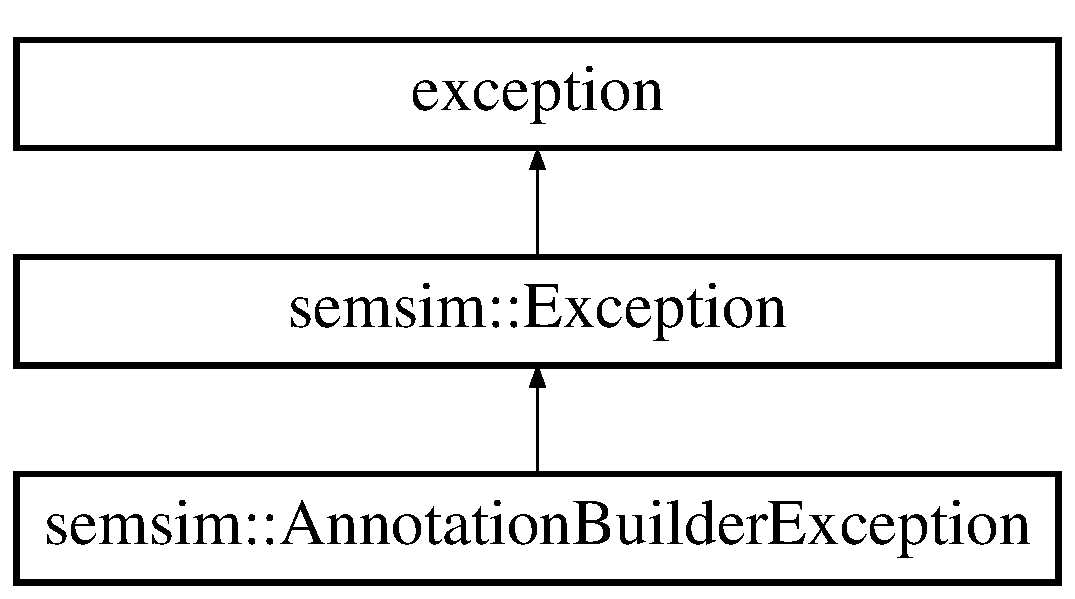
\includegraphics[height=3.000000cm]{classsemsim_1_1AnnotationBuilderException}
\end{center}
\end{figure}
\subsection*{Additional Inherited Members}


The documentation for this class was generated from the following file\+:\begin{DoxyCompactItemize}
\item 
src/semsim/Error.\+h\end{DoxyCompactItemize}

\hypertarget{classsemsim_1_1BiomodelsBiologyQualifier}{}\doxysection{semsim\+::Biomodels\+Biology\+Qualifier Class Reference}
\label{classsemsim_1_1BiomodelsBiologyQualifier}\index{semsim::BiomodelsBiologyQualifier@{semsim::BiomodelsBiologyQualifier}}
Inheritance diagram for semsim\+::Biomodels\+Biology\+Qualifier\+:\begin{figure}[H]
                                                                      \begin{center}
                                                                          \leavevmode
                                                                          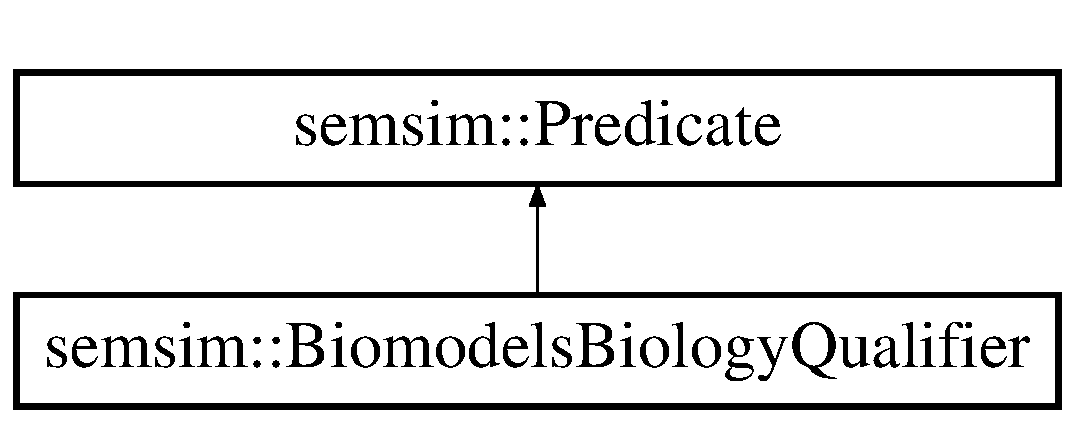
\includegraphics[height=2.000000cm]{classsemsim_1_1BiomodelsBiologyQualifier}
                                                                      \end{center}
\end{figure}
\doxysubsection*{Public Member Functions}
\begin{DoxyCompactItemize}
    \item
    \mbox{\Hypertarget{classsemsim_1_1BiomodelsBiologyQualifier_a4575502f2679dc01ce2280f829403c24}\label{classsemsim_1_1BiomodelsBiologyQualifier_a4575502f2679dc01ce2280f829403c24}}
    {\bfseries Biomodels\+Biology\+Qualifier} (Librdf\+World world, const std\+::string \&term)
\end{DoxyCompactItemize}
\doxysubsection*{Public Attributes}
\begin{DoxyCompactItemize}
    \item
    std\+::vector$<$ std\+::string $>$ {\bfseries valid\+\_\+terms\+\_\+}
\end{DoxyCompactItemize}
\doxysubsection*{Additional Inherited Members}


\doxysubsection{Member Data Documentation}
\mbox{\Hypertarget{classsemsim_1_1BiomodelsBiologyQualifier_a73a6b7ec962f32c4f03f292f23175440}\label{classsemsim_1_1BiomodelsBiologyQualifier_a73a6b7ec962f32c4f03f292f23175440}}
\index{semsim::BiomodelsBiologyQualifier@{semsim::BiomodelsBiologyQualifier}!valid\_terms\_@{valid\_terms\_}}
\index{valid\_terms\_@{valid\_terms\_}!semsim::BiomodelsBiologyQualifier@{semsim::BiomodelsBiologyQualifier}}
\doxysubsubsection{\texorpdfstring{valid\_terms\_}{valid\_terms\_}}
{\footnotesize\ttfamily std\+::vector$<$std\+::string$>$ semsim\+::\+Biomodels\+Biology\+Qualifier\+::valid\+\_\+terms\+\_\+}

{\bfseries Initial value\+:}
\begin{DoxyCode}{0}
    \DoxyCodeLine{\{}
    \DoxyCodeLine{                \textcolor{stringliteral}{"is"},}
    \DoxyCodeLine{                \textcolor{stringliteral}{"hasPart"},}
    \DoxyCodeLine{                \textcolor{stringliteral}{"isPartOf"},}
    \DoxyCodeLine{                \textcolor{stringliteral}{"isVersionOf"},}
    \DoxyCodeLine{                \textcolor{stringliteral}{"hasVersion"},}
    \DoxyCodeLine{                \textcolor{stringliteral}{"isHomologTo"},}
    \DoxyCodeLine{                \textcolor{stringliteral}{"isDescribedBy"},}
    \DoxyCodeLine{                \textcolor{stringliteral}{"isEncodedBy"},}
    \DoxyCodeLine{                \textcolor{stringliteral}{"encodes"},}
    \DoxyCodeLine{                \textcolor{stringliteral}{"occursIn"},}
    \DoxyCodeLine{                \textcolor{stringliteral}{"hasProperty"},}
    \DoxyCodeLine{                \textcolor{stringliteral}{"isPropertyOf"},}
    \DoxyCodeLine{                \textcolor{stringliteral}{"hasTaxon"}}
    \DoxyCodeLine{        \}}

\end{DoxyCode}


The documentation for this class was generated from the following files\+:\begin{DoxyCompactItemize}
                                                                              \item
                                                                              src/semsim/Predicate.\+h\item
                                                                              src/semsim/Predicate.\+cpp
\end{DoxyCompactItemize}

\hypertarget{classsemsim_1_1BiomodelsModelQualifier}{}\doxysection{semsim\+::Biomodels\+Model\+Qualifier Class Reference}
\label{classsemsim_1_1BiomodelsModelQualifier}\index{semsim::BiomodelsModelQualifier@{semsim::BiomodelsModelQualifier}}
Inheritance diagram for semsim\+::Biomodels\+Model\+Qualifier\+:\begin{figure}[H]
                                                                    \begin{center}
                                                                        \leavevmode
                                                                        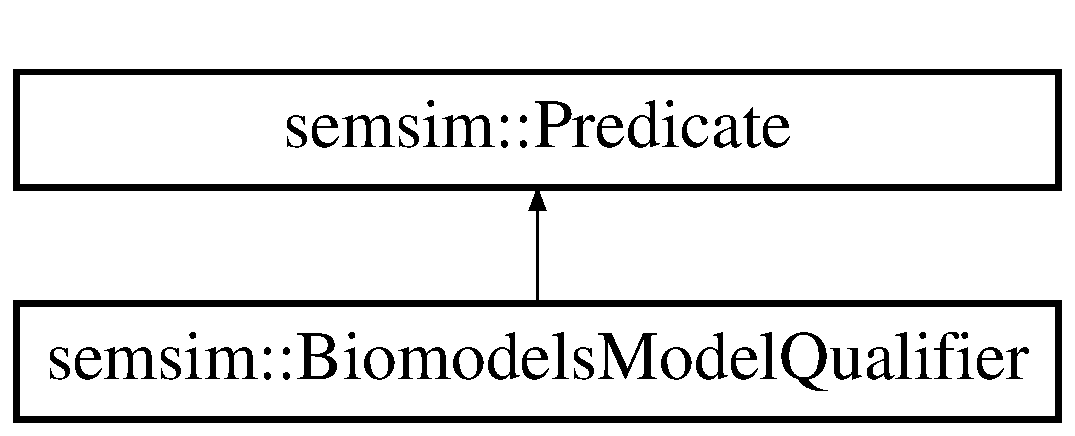
\includegraphics[height=2.000000cm]{classsemsim_1_1BiomodelsModelQualifier}
                                                                    \end{center}
\end{figure}
\doxysubsection*{Public Member Functions}
\begin{DoxyCompactItemize}
    \item
    \mbox{\Hypertarget{classsemsim_1_1BiomodelsModelQualifier_a705462b158ac0ac396bfd6786496d300}\label{classsemsim_1_1BiomodelsModelQualifier_a705462b158ac0ac396bfd6786496d300}}
    {\bfseries Biomodels\+Model\+Qualifier} (Librdf\+World world, const std\+::string \&term)
\end{DoxyCompactItemize}
\doxysubsection*{Public Attributes}
\begin{DoxyCompactItemize}
    \item
    std\+::vector$<$ std\+::string $>$ {\bfseries valid\+\_\+terms\+\_\+}
\end{DoxyCompactItemize}
\doxysubsection*{Additional Inherited Members}


\doxysubsection{Member Data Documentation}
\mbox{\Hypertarget{classsemsim_1_1BiomodelsModelQualifier_a6c270c5a9d8592180253a0e3a1e4f9ae}\label{classsemsim_1_1BiomodelsModelQualifier_a6c270c5a9d8592180253a0e3a1e4f9ae}}
\index{semsim::BiomodelsModelQualifier@{semsim::BiomodelsModelQualifier}!valid\_terms\_@{valid\_terms\_}}
\index{valid\_terms\_@{valid\_terms\_}!semsim::BiomodelsModelQualifier@{semsim::BiomodelsModelQualifier}}
\doxysubsubsection{\texorpdfstring{valid\_terms\_}{valid\_terms\_}}
{\footnotesize\ttfamily std\+::vector$<$std\+::string$>$ semsim\+::\+Biomodels\+Model\+Qualifier\+::valid\+\_\+terms\+\_\+}

{\bfseries Initial value\+:}
\begin{DoxyCode}{0}
    \DoxyCodeLine{\{}
    \DoxyCodeLine{                \textcolor{stringliteral}{"is"},}
    \DoxyCodeLine{                \textcolor{stringliteral}{"isDerivedFrom"},}
    \DoxyCodeLine{                \textcolor{stringliteral}{"isDescribedBy"},}
    \DoxyCodeLine{                \textcolor{stringliteral}{"isInstanceOf"},}
    \DoxyCodeLine{                \textcolor{stringliteral}{"hasInstance"},}
    \DoxyCodeLine{        \}}

\end{DoxyCode}


The documentation for this class was generated from the following files\+:\begin{DoxyCompactItemize}
                                                                              \item
                                                                              src/semsim/Predicate.\+h\item
                                                                              src/semsim/Predicate.\+cpp
\end{DoxyCompactItemize}

\hypertarget{classsemsim_1_1CellMLAssistant}{}\doxysection{semsim\+::Cell\+M\+L\+Assistant Class Reference}
\label{classsemsim_1_1CellMLAssistant}\index{semsim::CellMLAssistant@{semsim::CellMLAssistant}}
Inheritance diagram for semsim\+::Cell\+M\+L\+Assistant\+:\begin{figure}[H]
                                                              \begin{center}
                                                                  \leavevmode
                                                                  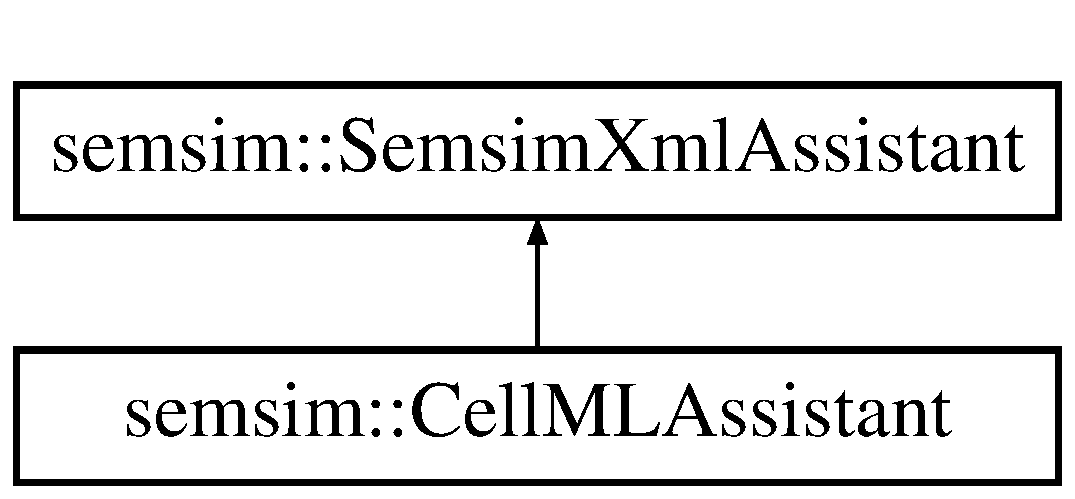
\includegraphics[height=2.000000cm]{classsemsim_1_1CellMLAssistant}
                                                              \end{center}
\end{figure}
\doxysubsection*{Public Member Functions}
\begin{DoxyCompactItemize}
    \item
    \mbox{\Hypertarget{classsemsim_1_1CellMLAssistant_a7c4eb903cc0143fa1d06b7fed802d054}\label{classsemsim_1_1CellMLAssistant_a7c4eb903cc0143fa1d06b7fed802d054}}
    const std\+::vector$<$ std\+::string $>$ \& {\bfseries get\+Valid\+Elements} () const override
    \item
    \mbox{\Hypertarget{classsemsim_1_1CellMLAssistant_a9616a091738c75e94e2ceb9f948f6b51}\label{classsemsim_1_1CellMLAssistant_a9616a091738c75e94e2ceb9f948f6b51}}
    {\bfseries Xml\+Assistant} (std\+::string xml, std\+::string base=\char`\"{}Meta\+ID\char`\"{}, int metaid\+\_\+num\+\_\+digits=4)
\end{DoxyCompactItemize}


The documentation for this class was generated from the following files\+:\begin{DoxyCompactItemize}
                                                                              \item
                                                                              src/semsim/Xml\+Assistant.\+h\item
                                                                              src/semsim/Xml\+Assistant.\+cpp
\end{DoxyCompactItemize}

\hypertarget{classsemsim_1_1CurlGet}{}\section{semsim\+:\+:Curl\+Get Class Reference}
\label{classsemsim_1_1CurlGet}\index{semsim\+::\+Curl\+Get@{semsim\+::\+Curl\+Get}}
\subsection*{Static Public Member Functions}
\begin{DoxyCompactItemize}
\item 
\mbox{\Hypertarget{classsemsim_1_1CurlGet_ab84cbd76261ce3b191a9442a539fd430}\label{classsemsim_1_1CurlGet_ab84cbd76261ce3b191a9442a539fd430}} 
static int {\bfseries download} (const std\+::string \&url, const std\+::string \&output\+\_\+filename)
\end{DoxyCompactItemize}


The documentation for this class was generated from the following files\+:\begin{DoxyCompactItemize}
\item 
src/semsim/Curl\+Get.\+h\item 
src/semsim/Curl\+Get.\+cpp\end{DoxyCompactItemize}

\hypertarget{classsemsim_1_1DCTerm}{}\section{semsim\+:\+:D\+C\+Term Class Reference}
\label{classsemsim_1_1DCTerm}\index{semsim\+::\+D\+C\+Term@{semsim\+::\+D\+C\+Term}}
Inheritance diagram for semsim\+:\+:D\+C\+Term\+:\begin{figure}[H]
\begin{center}
\leavevmode
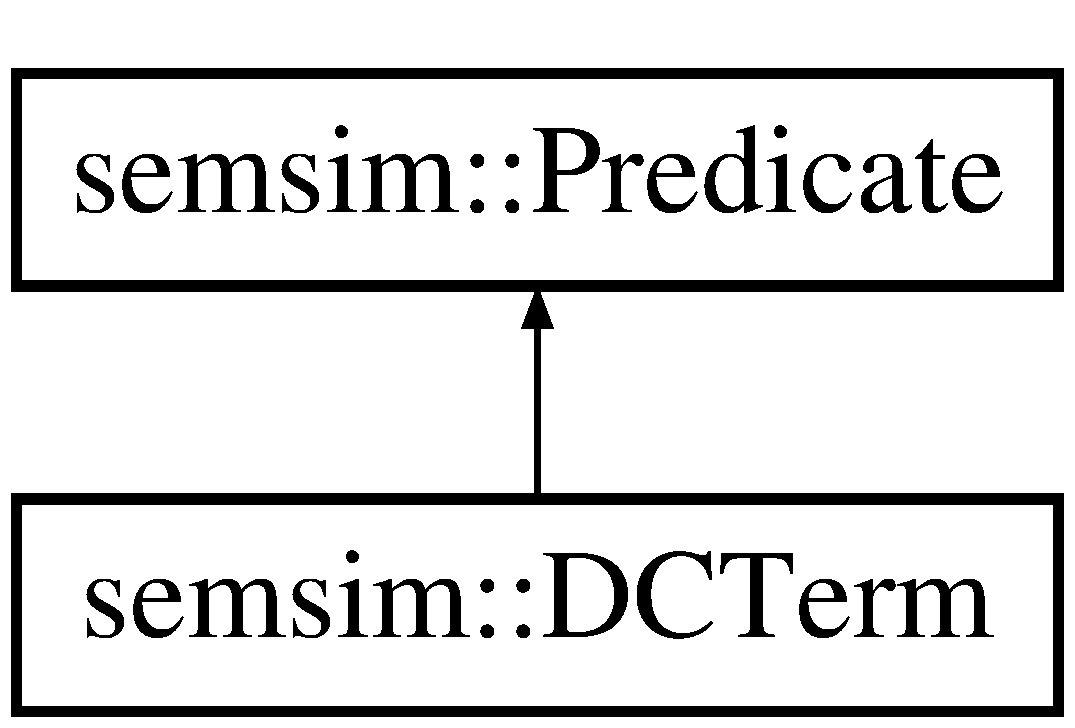
\includegraphics[height=2.000000cm]{classsemsim_1_1DCTerm}
\end{center}
\end{figure}
\subsection*{Public Member Functions}
\begin{DoxyCompactItemize}
\item 
\mbox{\Hypertarget{classsemsim_1_1DCTerm_a7ad576d21a2b4ddca2de1123fc9f5cd1}\label{classsemsim_1_1DCTerm_a7ad576d21a2b4ddca2de1123fc9f5cd1}} 
{\bfseries D\+C\+Term} (const std\+::string \&term)
\item 
\mbox{\Hypertarget{classsemsim_1_1DCTerm_a37a0aeaee6980ec00d51e686f0bd551b}\label{classsemsim_1_1DCTerm_a37a0aeaee6980ec00d51e686f0bd551b}} 
void {\bfseries verify} ()
\end{DoxyCompactItemize}
\subsection*{Public Attributes}
\begin{DoxyCompactItemize}
\item 
std\+::vector$<$ std\+::string $>$ {\bfseries valid\+\_\+terms\+\_\+}
\end{DoxyCompactItemize}
\subsection*{Additional Inherited Members}


\subsection{Member Data Documentation}
\mbox{\Hypertarget{classsemsim_1_1DCTerm_a09e8c38dd1a51c893ed92cca2e675475}\label{classsemsim_1_1DCTerm_a09e8c38dd1a51c893ed92cca2e675475}} 
\index{semsim\+::\+D\+C\+Term@{semsim\+::\+D\+C\+Term}!valid\+\_\+terms\+\_\+@{valid\+\_\+terms\+\_\+}}
\index{valid\+\_\+terms\+\_\+@{valid\+\_\+terms\+\_\+}!semsim\+::\+D\+C\+Term@{semsim\+::\+D\+C\+Term}}
\subsubsection{\texorpdfstring{valid\+\_\+terms\+\_\+}{valid\_terms\_}}
{\footnotesize\ttfamily std\+::vector$<$std\+::string$>$ semsim\+::\+D\+C\+Term\+::valid\+\_\+terms\+\_\+}

{\bfseries Initial value\+:}
\begin{DoxyCode}
\{
                \textcolor{stringliteral}{"Description"}
        \}
\end{DoxyCode}


The documentation for this class was generated from the following files\+:\begin{DoxyCompactItemize}
\item 
src/semsim/Predicate.\+h\item 
src/semsim/Predicate.\+cpp\end{DoxyCompactItemize}

\hypertarget{classsemsim_1_1Editor}{}\doxysection{semsim\+::Editor Class Reference}
\label{classsemsim_1_1Editor}\index{semsim::Editor@{semsim::Editor}}
\doxysubsection*{Public Member Functions}
\begin{DoxyCompactItemize}
    \item
    \mbox{\Hypertarget{classsemsim_1_1Editor_a41935516eed7c1a74d867c7d9001b9d9}\label{classsemsim_1_1Editor_a41935516eed7c1a74d867c7d9001b9d9}}
    const Namespace\+Map \& {\bfseries get\+Namespaces} () const
    \item
    \mbox{\Hypertarget{classsemsim_1_1Editor_a9b264ec07660c5c163a40bedd5ab903e}\label{classsemsim_1_1Editor_a9b264ec07660c5c163a40bedd5ab903e}}
    Librdf\+World {\bfseries get\+World} () const
    \item
    \mbox{\Hypertarget{classsemsim_1_1Editor_a2344dbf9775b1bc5968a7f6816e5e507}\label{classsemsim_1_1Editor_a2344dbf9775b1bc5968a7f6816e5e507}}
    Librdf\+Model {\bfseries get\+Model} () const
    \item
    \mbox{\Hypertarget{classsemsim_1_1Editor_aa67799c71119627bf2eb149777926619}\label{classsemsim_1_1Editor_aa67799c71119627bf2eb149777926619}}
    void {\bfseries set\+Namespaces} (const Namespace\+Map \&namespaces)
    \item
    \mbox{\Hypertarget{classsemsim_1_1Editor_ad807739b96bf8a11cf156cd655640d9e}\label{classsemsim_1_1Editor_ad807739b96bf8a11cf156cd655640d9e}}
    const Nested\+Triples \& {\bfseries get\+Triple\+List} () const
    \item
    \mbox{\Hypertarget{classsemsim_1_1Editor_a9f63d3e365758627b1af3edcd55065ac}\label{classsemsim_1_1Editor_a9f63d3e365758627b1af3edcd55065ac}}
    {\bfseries Editor} (const std\+::string \&xml, Xml\+Assistant\+Type type, Librdf\+World world, Librdf\+Model model, Namespace\+Map \&ns\+\_\+map)
    \item
    \mbox{\Hypertarget{classsemsim_1_1Editor_ac44d2a14cc890ab502897b8147d6a7f0}\label{classsemsim_1_1Editor_ac44d2a14cc890ab502897b8147d6a7f0}}
    const std\+::string \& {\bfseries get\+Xml} () const
    \item
    \mbox{\Hypertarget{classsemsim_1_1Editor_a442a53c7f01042a82307f161a9fb39aa}\label{classsemsim_1_1Editor_a442a53c7f01042a82307f161a9fb39aa}}
    const std\+::vector$<$ std\+::string $>$ \& {\bfseries get\+Metaids} () const
    \item
    \mbox{\Hypertarget{classsemsim_1_1Editor_a52f9cf039194b8aa64a56737398ce158}\label{classsemsim_1_1Editor_a52f9cf039194b8aa64a56737398ce158}}
    void {\bfseries add\+Single\+Annotation} (\mbox{\hyperlink{classsemsim_1_1Subject}{Subject}} subject, Predicate\+Ptr predicate\+\_\+ptr, \mbox{\hyperlink{classsemsim_1_1Resource}{Resource}} resource)
    \item
    \mbox{\Hypertarget{classsemsim_1_1Editor_ac9f7e88c9d94e7f557e0447de9bb80a1}\label{classsemsim_1_1Editor_ac9f7e88c9d94e7f557e0447de9bb80a1}}
    void {\bfseries add\+Namespace} (std\+::string ns, std\+::string prefix)
    \item
    \mbox{\Hypertarget{classsemsim_1_1Editor_ab555e053b2c49e97ab11e873bc38e949}\label{classsemsim_1_1Editor_ab555e053b2c49e97ab11e873bc38e949}}
    void {\bfseries add\+Single\+Annotation} (\mbox{\hyperlink{classsemsim_1_1Triple}{Singular\+Annotation}} singular\+Annotation)
    \item
    \mbox{\Hypertarget{classsemsim_1_1Editor_af4d4f32ca8dd1c7a952ec8887dfaf3d1}\label{classsemsim_1_1Editor_af4d4f32ca8dd1c7a952ec8887dfaf3d1}}
    void {\bfseries add\+Composite\+Annotation} (Physical\+Phenomenon\+Ptr phenomenon\+Ptr)
    \item
    \mbox{\Hypertarget{classsemsim_1_1Editor_abfe645502814173c412af776d3315e33}\label{classsemsim_1_1Editor_abfe645502814173c412af776d3315e33}}
    void {\bfseries add\+Physical\+Entity} (\mbox{\hyperlink{classsemsim_1_1PhysicalEntity}{Physical\+Entity}} physical\+Entity)
    \item
    \mbox{\Hypertarget{classsemsim_1_1Editor_adbe65d49835ddc3034cfb8529b76e50a}\label{classsemsim_1_1Editor_adbe65d49835ddc3034cfb8529b76e50a}}
    void {\bfseries add\+Physical\+Process} (\mbox{\hyperlink{classsemsim_1_1PhysicalProcess}{Physical\+Process}} physical\+Process)
    \item
    \mbox{\Hypertarget{classsemsim_1_1Editor_a7657fbbb87714526dfed15d3ae983350}\label{classsemsim_1_1Editor_a7657fbbb87714526dfed15d3ae983350}}
    void {\bfseries add\+Physical\+Force} (\mbox{\hyperlink{classsemsim_1_1PhysicalForce}{Physical\+Force}} physical\+Force)
    \item
    \mbox{\Hypertarget{classsemsim_1_1Editor_a577a1b6eb322412845f1b6e34b5c9990}\label{classsemsim_1_1Editor_a577a1b6eb322412845f1b6e34b5c9990}}
    void {\bfseries add\+Annotation\+From\+Nested\+Triples} (Nested\+Triples triple\+List)
    \item
    \mbox{\Hypertarget{classsemsim_1_1Editor_ae4d2ddb5f9c637bdaa9b65008bb00dfb}\label{classsemsim_1_1Editor_ae4d2ddb5f9c637bdaa9b65008bb00dfb}}
    void {\bfseries remove\+Annotation} (std\+::string metaid)
    \item
    \mbox{\Hypertarget{classsemsim_1_1Editor_a71f30e2cb766b0ad3ee4ed420cae4109}\label{classsemsim_1_1Editor_a71f30e2cb766b0ad3ee4ed420cae4109}}
    void {\bfseries to\+R\+DF} ()
    \item
    \mbox{\Hypertarget{classsemsim_1_1Editor_a3b02b6bfc728e4c36f74264295fba184}\label{classsemsim_1_1Editor_a3b02b6bfc728e4c36f74264295fba184}}
    void {\bfseries check\+Valid\+Metaid} (const std\+::string \&metaid)
    \item
    \mbox{\Hypertarget{classsemsim_1_1Editor_a05d70846b1d67decebe09a5dddfdf3eb}\label{classsemsim_1_1Editor_a05d70846b1d67decebe09a5dddfdf3eb}}
    void {\bfseries add\+Annotation\+From\+Triples} (\mbox{\hyperlink{classsemsim_1_1Triples}{Triples}} triples)
\end{DoxyCompactItemize}


The documentation for this class was generated from the following files\+:\begin{DoxyCompactItemize}
                                                                              \item
                                                                              src/semsim/Editor.\+h\item
                                                                              src/semsim/Editor.\+cpp
\end{DoxyCompactItemize}

\hypertarget{classException}{}\section{Exception Class Reference}
\label{classException}\index{Exception@{Exception}}
Inheritance diagram for Exception\+:\begin{figure}[H]
\begin{center}
\leavevmode
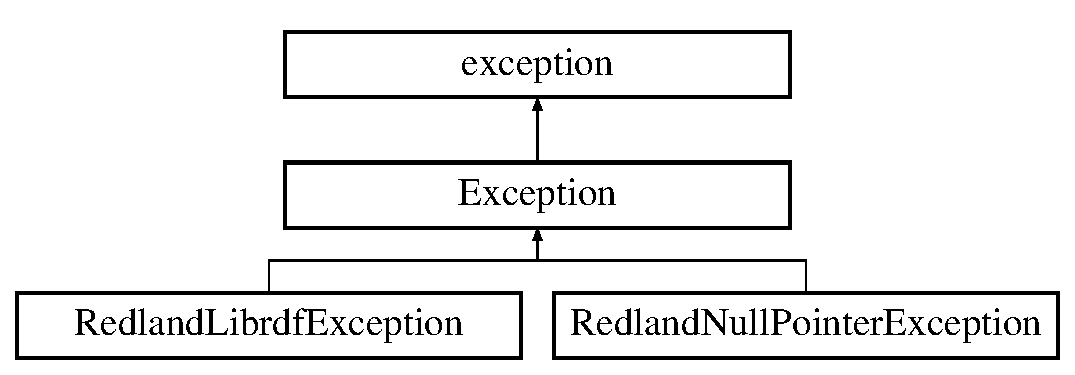
\includegraphics[height=3.000000cm]{classException}
\end{center}
\end{figure}
\subsection*{Public Member Functions}
\begin{DoxyCompactItemize}
\item 
\hyperlink{classException_ac541ead5c20548813d7dea73c28c7fab}{Exception} (const char $\ast$message)
\item 
\hyperlink{classException_a0b1693d4d5007815322070c907ee5cc2}{Exception} (std\+::string message)
\item 
\hyperlink{classException_ab834fdbc275748cf287b994503521ada}{$\sim$\+Exception} () noexcept override=default
\item 
const char $\ast$ \hyperlink{classException_ae7ba8334eb35e001b4b0c6df9339c0dc}{what} () const noexcept override
\end{DoxyCompactItemize}
\subsection*{Protected Attributes}
\begin{DoxyCompactItemize}
\item 
std\+::string \hyperlink{classException_a5d59cc46086c61391ed26773ce861780}{msg\+\_\+}
\end{DoxyCompactItemize}


\subsection{Constructor \& Destructor Documentation}
\mbox{\Hypertarget{classException_ac541ead5c20548813d7dea73c28c7fab}\label{classException_ac541ead5c20548813d7dea73c28c7fab}} 
\index{Exception@{Exception}!Exception@{Exception}}
\index{Exception@{Exception}!Exception@{Exception}}
\subsubsection{\texorpdfstring{Exception()}{Exception()}\hspace{0.1cm}{\footnotesize\ttfamily [1/2]}}
{\footnotesize\ttfamily Exception\+::\+Exception (\begin{DoxyParamCaption}\item[{const char $\ast$}]{message }\end{DoxyParamCaption})\hspace{0.3cm}{\ttfamily [inline]}, {\ttfamily [explicit]}}

Constructor (C strings). 
\begin{DoxyParams}{Parameters}
{\em message} & C-\/style string error message. The string contents are copied upon construction. Hence, responsibility for deleting the char$\ast$ lies with the caller. \\
\hline
\end{DoxyParams}
\mbox{\Hypertarget{classException_a0b1693d4d5007815322070c907ee5cc2}\label{classException_a0b1693d4d5007815322070c907ee5cc2}} 
\index{Exception@{Exception}!Exception@{Exception}}
\index{Exception@{Exception}!Exception@{Exception}}
\subsubsection{\texorpdfstring{Exception()}{Exception()}\hspace{0.1cm}{\footnotesize\ttfamily [2/2]}}
{\footnotesize\ttfamily Exception\+::\+Exception (\begin{DoxyParamCaption}\item[{std\+::string}]{message }\end{DoxyParamCaption})\hspace{0.3cm}{\ttfamily [inline]}, {\ttfamily [explicit]}}

Constructor (C++ S\+TL strings). 
\begin{DoxyParams}{Parameters}
{\em message} & The error message. \\
\hline
\end{DoxyParams}
\mbox{\Hypertarget{classException_ab834fdbc275748cf287b994503521ada}\label{classException_ab834fdbc275748cf287b994503521ada}} 
\index{Exception@{Exception}!````~Exception@{$\sim$\+Exception}}
\index{````~Exception@{$\sim$\+Exception}!Exception@{Exception}}
\subsubsection{\texorpdfstring{$\sim$\+Exception()}{~Exception()}}
{\footnotesize\ttfamily Exception\+::$\sim$\+Exception (\begin{DoxyParamCaption}{ }\end{DoxyParamCaption})\hspace{0.3cm}{\ttfamily [override]}, {\ttfamily [default]}, {\ttfamily [noexcept]}}

Destructor. Virtual to allow for subclassing. 

\subsection{Member Function Documentation}
\mbox{\Hypertarget{classException_ae7ba8334eb35e001b4b0c6df9339c0dc}\label{classException_ae7ba8334eb35e001b4b0c6df9339c0dc}} 
\index{Exception@{Exception}!what@{what}}
\index{what@{what}!Exception@{Exception}}
\subsubsection{\texorpdfstring{what()}{what()}}
{\footnotesize\ttfamily const char$\ast$ Exception\+::what (\begin{DoxyParamCaption}{ }\end{DoxyParamCaption}) const\hspace{0.3cm}{\ttfamily [inline]}, {\ttfamily [override]}, {\ttfamily [noexcept]}}

Returns a pointer to the (constant) error description. \begin{DoxyReturn}{Returns}
A pointer to a const char$\ast$. The underlying memory is in posession of the \hyperlink{classException}{Exception} object. Callers must not attempt to free the memory. 
\end{DoxyReturn}


\subsection{Member Data Documentation}
\mbox{\Hypertarget{classException_a5d59cc46086c61391ed26773ce861780}\label{classException_a5d59cc46086c61391ed26773ce861780}} 
\index{Exception@{Exception}!msg\+\_\+@{msg\+\_\+}}
\index{msg\+\_\+@{msg\+\_\+}!Exception@{Exception}}
\subsubsection{\texorpdfstring{msg\+\_\+}{msg\_}}
{\footnotesize\ttfamily std\+::string Exception\+::msg\+\_\+\hspace{0.3cm}{\ttfamily [protected]}}

Error message. 

The documentation for this class was generated from the following file\+:\begin{DoxyCompactItemize}
\item 
src/redland/\+Redland\+A\+P\+I\+Wrapper/src/Librdf\+Exception.\+h\end{DoxyCompactItemize}

\hypertarget{classsemsim_1_1Exception}{}\section{semsim\+:\+:Exception Class Reference}
\label{classsemsim_1_1Exception}\index{semsim\+::\+Exception@{semsim\+::\+Exception}}


\href{https://stackoverflow.com/questions/8152720/correct-way-to-inherit-from-stdexception}{\tt https\+://stackoverflow.\+com/questions/8152720/correct-\/way-\/to-\/inherit-\/from-\/stdexception}  




{\ttfamily \#include $<$Error.\+h$>$}

Inheritance diagram for semsim\+:\+:Exception\+:\begin{figure}[H]
\begin{center}
\leavevmode
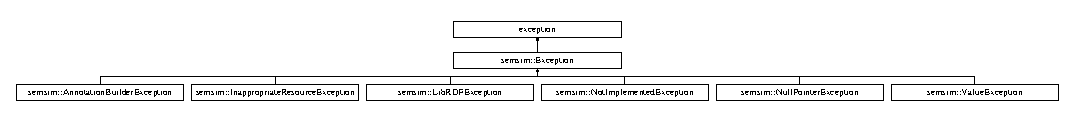
\includegraphics[height=1.120000cm]{classsemsim_1_1Exception}
\end{center}
\end{figure}
\subsection*{Public Member Functions}
\begin{DoxyCompactItemize}
\item 
\hyperlink{classsemsim_1_1Exception_ae32b373f579fc88ca9a9b406327f6549}{Exception} (const char $\ast$message)
\item 
\hyperlink{classsemsim_1_1Exception_acd15baba130b34cb81da8ce237406e99}{Exception} (std\+::string message)
\item 
\hyperlink{classsemsim_1_1Exception_a3f2c9347cddce32086f53f360a7839ae}{$\sim$\+Exception} () noexcept override=default
\item 
const char $\ast$ \hyperlink{classsemsim_1_1Exception_a301e9f6c7020ce7218811f4c0683ee77}{what} () const noexcept override
\end{DoxyCompactItemize}
\subsection*{Protected Attributes}
\begin{DoxyCompactItemize}
\item 
std\+::string \hyperlink{classsemsim_1_1Exception_a536284719db9cd57b8762e6e5a5a8820}{msg\+\_\+}
\end{DoxyCompactItemize}


\subsection{Detailed Description}
\href{https://stackoverflow.com/questions/8152720/correct-way-to-inherit-from-stdexception}{\tt https\+://stackoverflow.\+com/questions/8152720/correct-\/way-\/to-\/inherit-\/from-\/stdexception} 

\subsection{Constructor \& Destructor Documentation}
\mbox{\Hypertarget{classsemsim_1_1Exception_ae32b373f579fc88ca9a9b406327f6549}\label{classsemsim_1_1Exception_ae32b373f579fc88ca9a9b406327f6549}} 
\index{semsim\+::\+Exception@{semsim\+::\+Exception}!Exception@{Exception}}
\index{Exception@{Exception}!semsim\+::\+Exception@{semsim\+::\+Exception}}
\subsubsection{\texorpdfstring{Exception()}{Exception()}\hspace{0.1cm}{\footnotesize\ttfamily [1/2]}}
{\footnotesize\ttfamily semsim\+::\+Exception\+::\+Exception (\begin{DoxyParamCaption}\item[{const char $\ast$}]{message }\end{DoxyParamCaption})\hspace{0.3cm}{\ttfamily [inline]}, {\ttfamily [explicit]}}

Constructor (C strings). 
\begin{DoxyParams}{Parameters}
{\em message} & C-\/style string error message. The string contents are copied upon construction. Hence, responsibility for deleting the char$\ast$ lies with the caller. \\
\hline
\end{DoxyParams}
\mbox{\Hypertarget{classsemsim_1_1Exception_acd15baba130b34cb81da8ce237406e99}\label{classsemsim_1_1Exception_acd15baba130b34cb81da8ce237406e99}} 
\index{semsim\+::\+Exception@{semsim\+::\+Exception}!Exception@{Exception}}
\index{Exception@{Exception}!semsim\+::\+Exception@{semsim\+::\+Exception}}
\subsubsection{\texorpdfstring{Exception()}{Exception()}\hspace{0.1cm}{\footnotesize\ttfamily [2/2]}}
{\footnotesize\ttfamily semsim\+::\+Exception\+::\+Exception (\begin{DoxyParamCaption}\item[{std\+::string}]{message }\end{DoxyParamCaption})\hspace{0.3cm}{\ttfamily [inline]}, {\ttfamily [explicit]}}

Constructor (C++ S\+TL strings). 
\begin{DoxyParams}{Parameters}
{\em message} & The error message. \\
\hline
\end{DoxyParams}
\mbox{\Hypertarget{classsemsim_1_1Exception_a3f2c9347cddce32086f53f360a7839ae}\label{classsemsim_1_1Exception_a3f2c9347cddce32086f53f360a7839ae}} 
\index{semsim\+::\+Exception@{semsim\+::\+Exception}!````~Exception@{$\sim$\+Exception}}
\index{````~Exception@{$\sim$\+Exception}!semsim\+::\+Exception@{semsim\+::\+Exception}}
\subsubsection{\texorpdfstring{$\sim$\+Exception()}{~Exception()}}
{\footnotesize\ttfamily semsim\+::\+Exception\+::$\sim$\+Exception (\begin{DoxyParamCaption}{ }\end{DoxyParamCaption})\hspace{0.3cm}{\ttfamily [override]}, {\ttfamily [default]}, {\ttfamily [noexcept]}}

Destructor. Virtual to allow for subclassing. 

\subsection{Member Function Documentation}
\mbox{\Hypertarget{classsemsim_1_1Exception_a301e9f6c7020ce7218811f4c0683ee77}\label{classsemsim_1_1Exception_a301e9f6c7020ce7218811f4c0683ee77}} 
\index{semsim\+::\+Exception@{semsim\+::\+Exception}!what@{what}}
\index{what@{what}!semsim\+::\+Exception@{semsim\+::\+Exception}}
\subsubsection{\texorpdfstring{what()}{what()}}
{\footnotesize\ttfamily const char$\ast$ semsim\+::\+Exception\+::what (\begin{DoxyParamCaption}{ }\end{DoxyParamCaption}) const\hspace{0.3cm}{\ttfamily [inline]}, {\ttfamily [override]}, {\ttfamily [noexcept]}}

Returns a pointer to the (constant) error description. \begin{DoxyReturn}{Returns}
A pointer to a const char$\ast$. The underlying memory is in posession of the \hyperlink{classsemsim_1_1Exception}{Exception} object. Callers must not attempt to free the memory. 
\end{DoxyReturn}


\subsection{Member Data Documentation}
\mbox{\Hypertarget{classsemsim_1_1Exception_a536284719db9cd57b8762e6e5a5a8820}\label{classsemsim_1_1Exception_a536284719db9cd57b8762e6e5a5a8820}} 
\index{semsim\+::\+Exception@{semsim\+::\+Exception}!msg\+\_\+@{msg\+\_\+}}
\index{msg\+\_\+@{msg\+\_\+}!semsim\+::\+Exception@{semsim\+::\+Exception}}
\subsubsection{\texorpdfstring{msg\+\_\+}{msg\_}}
{\footnotesize\ttfamily std\+::string semsim\+::\+Exception\+::msg\+\_\+\hspace{0.3cm}{\ttfamily [protected]}}

Error message. 

The documentation for this class was generated from the following file\+:\begin{DoxyCompactItemize}
\item 
src/semsim/Error.\+h\end{DoxyCompactItemize}

\hypertarget{classsemsim_1_1InappropriateResourceException}{}\section{semsim\+:\+:Inappropriate\+Resource\+Exception Class Reference}
\label{classsemsim_1_1InappropriateResourceException}\index{semsim\+::\+Inappropriate\+Resource\+Exception@{semsim\+::\+Inappropriate\+Resource\+Exception}}
Inheritance diagram for semsim\+:\+:Inappropriate\+Resource\+Exception\+:\begin{figure}[H]
\begin{center}
\leavevmode
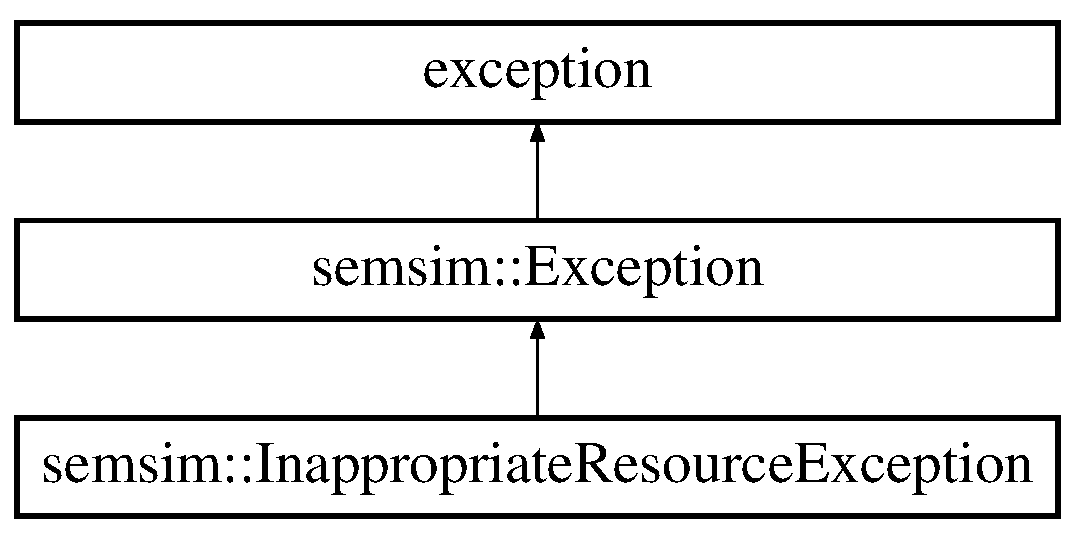
\includegraphics[height=3.000000cm]{classsemsim_1_1InappropriateResourceException}
\end{center}
\end{figure}
\subsection*{Additional Inherited Members}


The documentation for this class was generated from the following file\+:\begin{DoxyCompactItemize}
\item 
src/semsim/Error.\+h\end{DoxyCompactItemize}

\hypertarget{classsemsim_1_1LibRDFException}{}\doxysection{semsim\+::Lib\+R\+D\+F\+Exception Class Reference}
\label{classsemsim_1_1LibRDFException}\index{semsim::LibRDFException@{semsim::LibRDFException}}
Inheritance diagram for semsim\+::Lib\+R\+D\+F\+Exception\+:\begin{figure}[H]
                                                                \begin{center}
                                                                    \leavevmode
                                                                    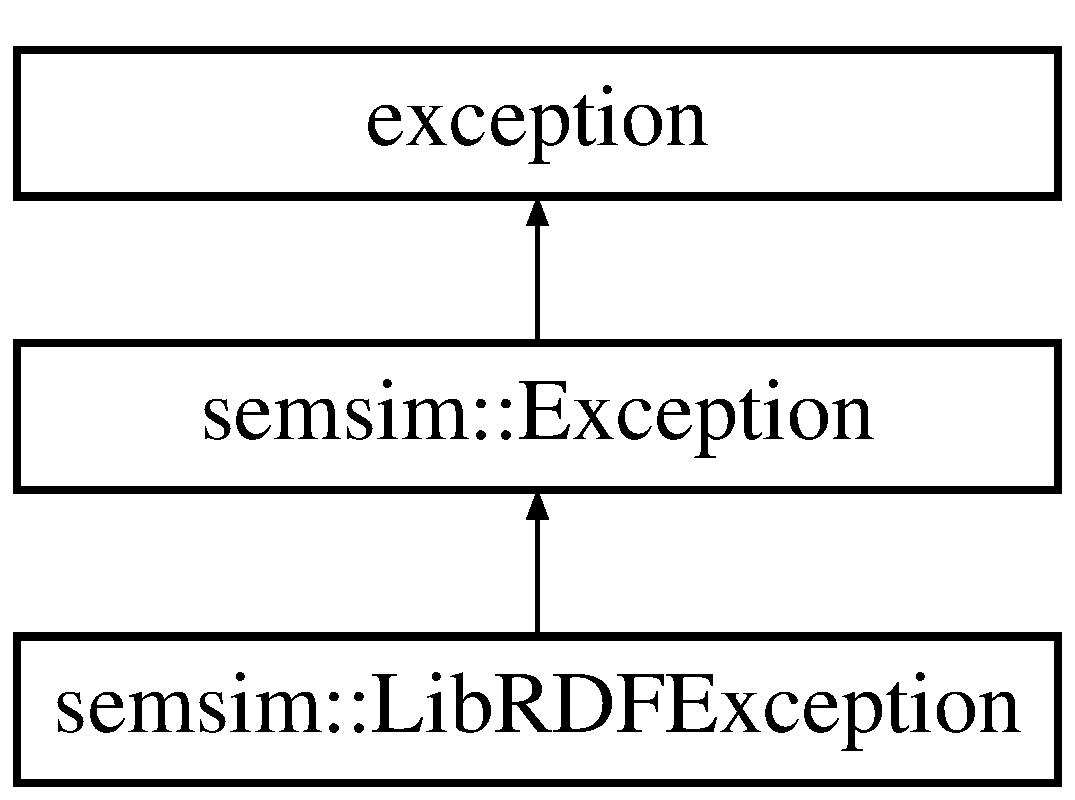
\includegraphics[height=3.000000cm]{classsemsim_1_1LibRDFException}
                                                                \end{center}
\end{figure}
\doxysubsection*{Additional Inherited Members}


The documentation for this class was generated from the following file\+:\begin{DoxyCompactItemize}
                                                                             \item
                                                                             src/semsim/Error.\+h
\end{DoxyCompactItemize}

\hypertarget{classredland_1_1LibrdfModel}{}\section{redland\+:\+:Librdf\+Model Class Reference}
\label{classredland_1_1LibrdfModel}\index{redland\+::\+Librdf\+Model@{redland\+::\+Librdf\+Model}}
\subsection*{Public Member Functions}
\begin{DoxyCompactItemize}
\item 
\mbox{\Hypertarget{classredland_1_1LibrdfModel_a5a35c032585e38b1d41bc18f057128c1}\label{classredland_1_1LibrdfModel_a5a35c032585e38b1d41bc18f057128c1}} 
{\bfseries Librdf\+Model} (const \hyperlink{classredland_1_1LibrdfModel}{Librdf\+Model} \&model)=delete
\item 
\mbox{\Hypertarget{classredland_1_1LibrdfModel_a583e0eaecfe167ccbbeac5d768bcd644}\label{classredland_1_1LibrdfModel_a583e0eaecfe167ccbbeac5d768bcd644}} 
{\bfseries Librdf\+Model} (\hyperlink{classredland_1_1LibrdfModel}{Librdf\+Model} \&\&model) noexcept
\item 
\mbox{\Hypertarget{classredland_1_1LibrdfModel_a7bd07324b31fa8eb8f5f2e51b15044fc}\label{classredland_1_1LibrdfModel_a7bd07324b31fa8eb8f5f2e51b15044fc}} 
\hyperlink{classredland_1_1LibrdfModel}{Librdf\+Model} \& {\bfseries operator=} (const \hyperlink{classredland_1_1LibrdfModel}{Librdf\+Model} \&model)=delete
\item 
\mbox{\Hypertarget{classredland_1_1LibrdfModel_a9007acfb92943e018d20d6985c811033}\label{classredland_1_1LibrdfModel_a9007acfb92943e018d20d6985c811033}} 
\hyperlink{classredland_1_1LibrdfModel}{Librdf\+Model} \& {\bfseries operator=} (\hyperlink{classredland_1_1LibrdfModel}{Librdf\+Model} \&\&model) noexcept
\item 
\mbox{\Hypertarget{classredland_1_1LibrdfModel_a8b7d3063e030ce8613dcd6def7463a5a}\label{classredland_1_1LibrdfModel_a8b7d3063e030ce8613dcd6def7463a5a}} 
{\bfseries Librdf\+Model} (librdf\+\_\+model $\ast$model)
\item 
\mbox{\Hypertarget{classredland_1_1LibrdfModel_a355e16664fa50a8a3085f4070347106f}\label{classredland_1_1LibrdfModel_a355e16664fa50a8a3085f4070347106f}} 
{\bfseries Librdf\+Model} (librdf\+\_\+storage $\ast$storage, const char $\ast$options=nullptr)
\item 
\mbox{\Hypertarget{classredland_1_1LibrdfModel_ae1b996f1785adfe9b4a1824a73643248}\label{classredland_1_1LibrdfModel_ae1b996f1785adfe9b4a1824a73643248}} 
librdf\+\_\+model $\ast$ {\bfseries get} () const
\item 
\mbox{\Hypertarget{classredland_1_1LibrdfModel_a29e79bafe40a64141ab7edf8ecbbbdd3}\label{classredland_1_1LibrdfModel_a29e79bafe40a64141ab7edf8ecbbbdd3}} 
\hyperlink{classredland_1_1LibrdfQueryResults}{Librdf\+Query\+Results} {\bfseries query} (\hyperlink{classredland_1_1LibrdfQuery}{Librdf\+Query} query)
\item 
\mbox{\Hypertarget{classredland_1_1LibrdfModel_a646ed92896c4030de31c9e17b881bd2a}\label{classredland_1_1LibrdfModel_a646ed92896c4030de31c9e17b881bd2a}} 
\hyperlink{classredland_1_1LibrdfStream}{Librdf\+Stream} {\bfseries to\+Stream} ()
\item 
\mbox{\Hypertarget{classredland_1_1LibrdfModel_a3067eb5bae1353ab5c86f135c4b401ad}\label{classredland_1_1LibrdfModel_a3067eb5bae1353ab5c86f135c4b401ad}} 
int {\bfseries size} () const
\item 
\mbox{\Hypertarget{classredland_1_1LibrdfModel_a2b565a7d705e24d6163c068a40040087}\label{classredland_1_1LibrdfModel_a2b565a7d705e24d6163c068a40040087}} 
void {\bfseries add\+Statement} (const \hyperlink{classredland_1_1LibrdfStatement}{Librdf\+Statement} \&statement) const
\item 
\mbox{\Hypertarget{classredland_1_1LibrdfModel_a643c3e3d3363f4f06330ede73dc19514}\label{classredland_1_1LibrdfModel_a643c3e3d3363f4f06330ede73dc19514}} 
void {\bfseries add\+Statement} (librdf\+\_\+statement $\ast$statement) const
\item 
\mbox{\Hypertarget{classredland_1_1LibrdfModel_ad145b8f46be49434bb8bd0b90a904770}\label{classredland_1_1LibrdfModel_ad145b8f46be49434bb8bd0b90a904770}} 
void {\bfseries free\+Model} ()
\end{DoxyCompactItemize}


The documentation for this class was generated from the following files\+:\begin{DoxyCompactItemize}
\item 
src/redland/\+Redland\+A\+P\+I\+Wrapper/src/Librdf\+Model.\+h\item 
src/redland/\+Redland\+A\+P\+I\+Wrapper/src/Librdf\+Model.\+cpp\end{DoxyCompactItemize}

\hypertarget{classredland_1_1LibrdfNode}{}\section{redland\+:\+:Librdf\+Node Class Reference}
\label{classredland_1_1LibrdfNode}\index{redland\+::\+Librdf\+Node@{redland\+::\+Librdf\+Node}}
\subsection*{Public Member Functions}
\begin{DoxyCompactItemize}
\item 
\mbox{\Hypertarget{classredland_1_1LibrdfNode_a28f6ce060bddf7e1cb88d17d4d4ea81a}\label{classredland_1_1LibrdfNode_a28f6ce060bddf7e1cb88d17d4d4ea81a}} 
void {\bfseries free\+Node} ()
\item 
\mbox{\Hypertarget{classredland_1_1LibrdfNode_a669557dc1240dc17c3a7a3a61d2400d9}\label{classredland_1_1LibrdfNode_a669557dc1240dc17c3a7a3a61d2400d9}} 
{\bfseries Librdf\+Node} (const \hyperlink{classredland_1_1LibrdfNode}{Librdf\+Node} \&node)=delete
\item 
\mbox{\Hypertarget{classredland_1_1LibrdfNode_a822ce6a4221315abe5768b278b83d0e5}\label{classredland_1_1LibrdfNode_a822ce6a4221315abe5768b278b83d0e5}} 
{\bfseries Librdf\+Node} (\hyperlink{classredland_1_1LibrdfNode}{Librdf\+Node} \&\&node) noexcept
\item 
\mbox{\Hypertarget{classredland_1_1LibrdfNode_abce52c34cc89e48886cde07aa5e113c9}\label{classredland_1_1LibrdfNode_abce52c34cc89e48886cde07aa5e113c9}} 
\hyperlink{classredland_1_1LibrdfNode}{Librdf\+Node} \& {\bfseries operator=} (const \hyperlink{classredland_1_1LibrdfNode}{Librdf\+Node} \&node)=delete
\item 
\mbox{\Hypertarget{classredland_1_1LibrdfNode_a9de3a69b00958b2bb50646dbf0aa8d7e}\label{classredland_1_1LibrdfNode_a9de3a69b00958b2bb50646dbf0aa8d7e}} 
\hyperlink{classredland_1_1LibrdfNode}{Librdf\+Node} \& {\bfseries operator=} (\hyperlink{classredland_1_1LibrdfNode}{Librdf\+Node} \&\&node) noexcept
\item 
\mbox{\Hypertarget{classredland_1_1LibrdfNode_a200c7a67088e66d6fc73f52bdb51d2e9}\label{classredland_1_1LibrdfNode_a200c7a67088e66d6fc73f52bdb51d2e9}} 
{\bfseries Librdf\+Node} (librdf\+\_\+node $\ast$node)
\item 
\mbox{\Hypertarget{classredland_1_1LibrdfNode_a33162ea36efe451c100325816cf8613f}\label{classredland_1_1LibrdfNode_a33162ea36efe451c100325816cf8613f}} 
librdf\+\_\+node $\ast$ {\bfseries get} () const
\item 
\mbox{\Hypertarget{classredland_1_1LibrdfNode_a83ec604f27e71cea80ac49569a06ddfe}\label{classredland_1_1LibrdfNode_a83ec604f27e71cea80ac49569a06ddfe}} 
raptor\+\_\+term\+\_\+type {\bfseries get\+Raptor\+Term\+Type} ()
\item 
\mbox{\Hypertarget{classredland_1_1LibrdfNode_a528bc0251daa0907e4891fe06e47c567}\label{classredland_1_1LibrdfNode_a528bc0251daa0907e4891fe06e47c567}} 
std\+::string {\bfseries str} ()
\item 
\mbox{\Hypertarget{classredland_1_1LibrdfNode_a98487d5af58971d820fcb99c88d8712d}\label{classredland_1_1LibrdfNode_a98487d5af58971d820fcb99c88d8712d}} 
\hyperlink{classredland_1_1LibrdfUri}{Librdf\+Uri} {\bfseries get\+Literal\+Datatype} ()
\item 
\mbox{\Hypertarget{classredland_1_1LibrdfNode_a58b9962c783be77fd0d2cb7036bfdc6a}\label{classredland_1_1LibrdfNode_a58b9962c783be77fd0d2cb7036bfdc6a}} 
std\+::string {\bfseries get\+Literal\+Language} ()
\item 
\mbox{\Hypertarget{classredland_1_1LibrdfNode_a49431de8c3262ee56d533a5fe047ee00}\label{classredland_1_1LibrdfNode_a49431de8c3262ee56d533a5fe047ee00}} 
std\+::string {\bfseries get\+Blank\+Identifier} ()
\item 
\mbox{\Hypertarget{classredland_1_1LibrdfNode_a0dd2ff697c0753eddf7327f64390ed77}\label{classredland_1_1LibrdfNode_a0dd2ff697c0753eddf7327f64390ed77}} 
\hyperlink{classredland_1_1LibrdfUri}{Librdf\+Uri} {\bfseries get\+Uri} ()
\item 
\mbox{\Hypertarget{classredland_1_1LibrdfNode_a01aeb7675187379674746f803a1fbdc9}\label{classredland_1_1LibrdfNode_a01aeb7675187379674746f803a1fbdc9}} 
void {\bfseries set\+Uri} (const std\+::string \&uri)
\item 
\mbox{\Hypertarget{classredland_1_1LibrdfNode_a160db9f7c7636c339e12c26f519b8fff}\label{classredland_1_1LibrdfNode_a160db9f7c7636c339e12c26f519b8fff}} 
void {\bfseries set\+Literal\+Datatype} (const std\+::string \&datatype)
\item 
\mbox{\Hypertarget{classredland_1_1LibrdfNode_afd81499fe4125cc2f4c472d33fb6c8c0}\label{classredland_1_1LibrdfNode_afd81499fe4125cc2f4c472d33fb6c8c0}} 
void {\bfseries set\+Blank\+Identifier} (const std\+::string \&identifier)
\end{DoxyCompactItemize}
\subsection*{Static Public Member Functions}
\begin{DoxyCompactItemize}
\item 
\mbox{\Hypertarget{classredland_1_1LibrdfNode_a5c971e6daeca94c4eabddfa5f6e4c456}\label{classredland_1_1LibrdfNode_a5c971e6daeca94c4eabddfa5f6e4c456}} 
static void {\bfseries free\+Node} (librdf\+\_\+node $\ast$node)
\item 
\mbox{\Hypertarget{classredland_1_1LibrdfNode_aacf853ee60f9d706bc7e95fb426166bd}\label{classredland_1_1LibrdfNode_aacf853ee60f9d706bc7e95fb426166bd}} 
static \hyperlink{classredland_1_1LibrdfNode}{Librdf\+Node} {\bfseries from\+Uri\+String} (const std\+::string \&uri\+\_\+string)
\item 
\mbox{\Hypertarget{classredland_1_1LibrdfNode_a22ea96262be432e6abb5c1e28ede3071}\label{classredland_1_1LibrdfNode_a22ea96262be432e6abb5c1e28ede3071}} 
static \hyperlink{classredland_1_1LibrdfNode}{Librdf\+Node} {\bfseries from\+Blank} (const std\+::string \&blank)
\item 
\mbox{\Hypertarget{classredland_1_1LibrdfNode_a346fad618a010ef983ce24d62891de0e}\label{classredland_1_1LibrdfNode_a346fad618a010ef983ce24d62891de0e}} 
static \hyperlink{classredland_1_1LibrdfNode}{Librdf\+Node} {\bfseries from\+Literal} (const std\+::string \&literal, const std\+::string \&literal\+\_\+datatype\+\_\+uri=\char`\"{}string\char`\"{}, const std\+::string \&xml\+\_\+language=std\+::string())
\item 
\mbox{\Hypertarget{classredland_1_1LibrdfNode_aa6bf7e25e68e473f2f39cb7b4cb5f39b}\label{classredland_1_1LibrdfNode_aa6bf7e25e68e473f2f39cb7b4cb5f39b}} 
static std\+::string {\bfseries str} (librdf\+\_\+node $\ast$node)
\item 
\mbox{\Hypertarget{classredland_1_1LibrdfNode_a3242e29edb736ba0aa8ac42fd6b3ae58}\label{classredland_1_1LibrdfNode_a3242e29edb736ba0aa8ac42fd6b3ae58}} 
static std\+::string {\bfseries validate\+Literal\+Datatype} (const std\+::string \&literal\+\_\+datatype\+\_\+uri)
\end{DoxyCompactItemize}


The documentation for this class was generated from the following files\+:\begin{DoxyCompactItemize}
\item 
src/redland/\+Redland\+A\+P\+I\+Wrapper/src/Librdf\+Node.\+h\item 
src/redland/\+Redland\+A\+P\+I\+Wrapper/src/Librdf\+Node.\+cpp\end{DoxyCompactItemize}

\hypertarget{classredland_1_1LibrdfParser}{}\section{redland\+:\+:Librdf\+Parser Class Reference}
\label{classredland_1_1LibrdfParser}\index{redland\+::\+Librdf\+Parser@{redland\+::\+Librdf\+Parser}}
\subsection*{Public Member Functions}
\begin{DoxyCompactItemize}
\item 
\mbox{\Hypertarget{classredland_1_1LibrdfParser_a884b4e7cb05942390fba7765cfb3aec8}\label{classredland_1_1LibrdfParser_a884b4e7cb05942390fba7765cfb3aec8}} 
{\bfseries Librdf\+Parser} (const \hyperlink{classredland_1_1LibrdfParser}{Librdf\+Parser} \&parser)=delete
\item 
\mbox{\Hypertarget{classredland_1_1LibrdfParser_a8c75ee321bd82076491aa0d63d0664c8}\label{classredland_1_1LibrdfParser_a8c75ee321bd82076491aa0d63d0664c8}} 
{\bfseries Librdf\+Parser} (\hyperlink{classredland_1_1LibrdfParser}{Librdf\+Parser} \&\&parser) noexcept
\item 
\mbox{\Hypertarget{classredland_1_1LibrdfParser_aeee1312383f2e3f72e49076390a2a27b}\label{classredland_1_1LibrdfParser_aeee1312383f2e3f72e49076390a2a27b}} 
\hyperlink{classredland_1_1LibrdfParser}{Librdf\+Parser} \& {\bfseries operator=} (const \hyperlink{classredland_1_1LibrdfParser}{Librdf\+Parser} \&parser)=delete
\item 
\mbox{\Hypertarget{classredland_1_1LibrdfParser_a5a5e09075b43906c9161d453ac63ab8a}\label{classredland_1_1LibrdfParser_a5a5e09075b43906c9161d453ac63ab8a}} 
\hyperlink{classredland_1_1LibrdfParser}{Librdf\+Parser} \& {\bfseries operator=} (\hyperlink{classredland_1_1LibrdfParser}{Librdf\+Parser} \&\&parser) noexcept
\item 
\mbox{\Hypertarget{classredland_1_1LibrdfParser_ac1373b22444c108a2a67dbf24fa4ca92}\label{classredland_1_1LibrdfParser_ac1373b22444c108a2a67dbf24fa4ca92}} 
{\bfseries Librdf\+Parser} (librdf\+\_\+parser $\ast$parser)
\item 
\mbox{\Hypertarget{classredland_1_1LibrdfParser_afa206d1b923c66ecc206afe83834382e}\label{classredland_1_1LibrdfParser_afa206d1b923c66ecc206afe83834382e}} 
{\bfseries Librdf\+Parser} (std\+::string format, std\+::string mime\+\_\+type=std\+::string(), std\+::string type\+\_\+uri=std\+::string())
\item 
\mbox{\Hypertarget{classredland_1_1LibrdfParser_aadb297b986879ca618d3092fe737d41c}\label{classredland_1_1LibrdfParser_aadb297b986879ca618d3092fe737d41c}} 
librdf\+\_\+parser $\ast$ {\bfseries get} () const
\item 
\mbox{\Hypertarget{classredland_1_1LibrdfParser_aa00b1ab4b50a7d5469dd012752ed4dc8}\label{classredland_1_1LibrdfParser_aa00b1ab4b50a7d5469dd012752ed4dc8}} 
void {\bfseries set\+Feature} (std\+::string feature\+\_\+uri, \hyperlink{classredland_1_1LibrdfNode}{Librdf\+Node} node) const
\item 
\mbox{\Hypertarget{classredland_1_1LibrdfParser_a1e2098e2c99ba886ab1521048258600c}\label{classredland_1_1LibrdfParser_a1e2098e2c99ba886ab1521048258600c}} 
int {\bfseries num\+Namespaces\+Seen} () const
\item 
\mbox{\Hypertarget{classredland_1_1LibrdfParser_aed92021f88bccfa26bf78c29797b4208}\label{classredland_1_1LibrdfParser_aed92021f88bccfa26bf78c29797b4208}} 
std\+::string {\bfseries get\+Namespaces\+Seen\+Uri} (int index) const
\item 
\mbox{\Hypertarget{classredland_1_1LibrdfParser_a86739506ba32a9a6da8b69711f1026db}\label{classredland_1_1LibrdfParser_a86739506ba32a9a6da8b69711f1026db}} 
void {\bfseries parse\+String} (const std\+::string \&rdf\+\_\+string, const \hyperlink{classredland_1_1LibrdfModel}{Librdf\+Model} \&model, const \hyperlink{classredland_1_1LibrdfUri}{Librdf\+Uri} \&base\+\_\+uri) const
\item 
\mbox{\Hypertarget{classredland_1_1LibrdfParser_a2a7ac5ac97b4bc5876db02f0b9c7b987}\label{classredland_1_1LibrdfParser_a2a7ac5ac97b4bc5876db02f0b9c7b987}} 
void {\bfseries parse\+String} (const std\+::string \&rdf\+\_\+string, const \hyperlink{classredland_1_1LibrdfModel}{Librdf\+Model} \&model, const std\+::string \&base\+\_\+uri) const
\item 
\mbox{\Hypertarget{classredland_1_1LibrdfParser_a15ffb21bf48e486708eab820719827a6}\label{classredland_1_1LibrdfParser_a15ffb21bf48e486708eab820719827a6}} 
void {\bfseries parse\+File} (const std\+::string \&filename\+\_\+uri, const \hyperlink{classredland_1_1LibrdfModel}{Librdf\+Model} \&model) const
\item 
\mbox{\Hypertarget{classredland_1_1LibrdfParser_a733bf5d33a2d71bd6d7c201e1c952b04}\label{classredland_1_1LibrdfParser_a733bf5d33a2d71bd6d7c201e1c952b04}} 
void {\bfseries parse\+Uri} (const std\+::string \&uri\+\_\+string, const \hyperlink{classredland_1_1LibrdfModel}{Librdf\+Model} \&model) const
\item 
\mbox{\Hypertarget{classredland_1_1LibrdfParser_a89d1335343c9999db8207866de8202c1}\label{classredland_1_1LibrdfParser_a89d1335343c9999db8207866de8202c1}} 
std\+::string {\bfseries get\+Namespaces\+Seen\+Prefix} (int index) const
\item 
\mbox{\Hypertarget{classredland_1_1LibrdfParser_aaa813cd98f57703e2168e81cf1c8b356}\label{classredland_1_1LibrdfParser_aaa813cd98f57703e2168e81cf1c8b356}} 
std\+::string {\bfseries get\+Name} () const
\item 
\mbox{\Hypertarget{classredland_1_1LibrdfParser_a152feb7bf2aa291fc7ec48fe2769265a}\label{classredland_1_1LibrdfParser_a152feb7bf2aa291fc7ec48fe2769265a}} 
void {\bfseries set\+Name} (const char $\ast$name)
\item 
\mbox{\Hypertarget{classredland_1_1LibrdfParser_aacf1514391f15d3687a35352f1c0da3d}\label{classredland_1_1LibrdfParser_aacf1514391f15d3687a35352f1c0da3d}} 
std\+::string {\bfseries get\+Mime\+Type} () const
\item 
\mbox{\Hypertarget{classredland_1_1LibrdfParser_a8fe0e89950e9b71f86fa58e10eb475d8}\label{classredland_1_1LibrdfParser_a8fe0e89950e9b71f86fa58e10eb475d8}} 
void {\bfseries set\+Mime\+Type} (const char $\ast$mime\+Type)
\item 
\mbox{\Hypertarget{classredland_1_1LibrdfParser_ae6f233d632e3a515afe7afceabf4e5ef}\label{classredland_1_1LibrdfParser_ae6f233d632e3a515afe7afceabf4e5ef}} 
librdf\+\_\+uri $\ast$ {\bfseries get\+Type\+Uri} () const
\item 
\mbox{\Hypertarget{classredland_1_1LibrdfParser_a81d772e0be266b00bf840fd9dbeab8d1}\label{classredland_1_1LibrdfParser_a81d772e0be266b00bf840fd9dbeab8d1}} 
void {\bfseries set\+Type\+Uri} (librdf\+\_\+uri $\ast$type\+Uri)
\item 
\mbox{\Hypertarget{classredland_1_1LibrdfParser_a76ecf31cd9fb96ba4e10a35f383e47fc}\label{classredland_1_1LibrdfParser_a76ecf31cd9fb96ba4e10a35f383e47fc}} 
void {\bfseries set\+Type\+Uri} (const std\+::string \&type\+\_\+uri)
\item 
\mbox{\Hypertarget{classredland_1_1LibrdfParser_a8055c22ada8b852112f4f011d9fa5abe}\label{classredland_1_1LibrdfParser_a8055c22ada8b852112f4f011d9fa5abe}} 
librdf\+\_\+parser $\ast$ {\bfseries make\+Parser} ()
\item 
\mbox{\Hypertarget{classredland_1_1LibrdfParser_a2c600b9ae3b59e4ae7e48b20e3513cb4}\label{classredland_1_1LibrdfParser_a2c600b9ae3b59e4ae7e48b20e3513cb4}} 
std\+::vector$<$ std\+::string $>$ {\bfseries get\+Seen\+Namespaces} () const
\end{DoxyCompactItemize}
\subsection*{Static Public Member Functions}
\begin{DoxyCompactItemize}
\item 
\mbox{\Hypertarget{classredland_1_1LibrdfParser_adcca22d570842637f601c19256f67c2b}\label{classredland_1_1LibrdfParser_adcca22d570842637f601c19256f67c2b}} 
static void {\bfseries set\+Feature} (librdf\+\_\+parser $\ast$parser, const std\+::string \&feature\+\_\+uri, librdf\+\_\+node $\ast$node)
\item 
\mbox{\Hypertarget{classredland_1_1LibrdfParser_aafc4a6e2748ee1175471ed0815d77eff}\label{classredland_1_1LibrdfParser_aafc4a6e2748ee1175471ed0815d77eff}} 
static void {\bfseries set\+Option} (librdf\+\_\+parser $\ast$parser, const std\+::string \&option, const std\+::string \&value)
\item 
\mbox{\Hypertarget{classredland_1_1LibrdfParser_a79fcda1e0c2cccfa8a070a1aea196ebd}\label{classredland_1_1LibrdfParser_a79fcda1e0c2cccfa8a070a1aea196ebd}} 
static void {\bfseries set\+Options} (librdf\+\_\+parser $\ast$parser)
\end{DoxyCompactItemize}


The documentation for this class was generated from the following files\+:\begin{DoxyCompactItemize}
\item 
src/redland/\+Redland\+A\+P\+I\+Wrapper/src/Librdf\+Parser.\+h\item 
src/redland/\+Redland\+A\+P\+I\+Wrapper/src/Librdf\+Parser.\+cpp\end{DoxyCompactItemize}

\hypertarget{classredland_1_1LibrdfQuery}{}\section{redland\+:\+:Librdf\+Query Class Reference}
\label{classredland_1_1LibrdfQuery}\index{redland\+::\+Librdf\+Query@{redland\+::\+Librdf\+Query}}
\subsection*{Public Member Functions}
\begin{DoxyCompactItemize}
\item 
\mbox{\Hypertarget{classredland_1_1LibrdfQuery_aacca5302206092fbd8908934d2236021}\label{classredland_1_1LibrdfQuery_aacca5302206092fbd8908934d2236021}} 
{\bfseries Librdf\+Query} (librdf\+\_\+query $\ast$query)
\item 
\mbox{\Hypertarget{classredland_1_1LibrdfQuery_a63a49930cc3c54938203683eab2c96fb}\label{classredland_1_1LibrdfQuery_a63a49930cc3c54938203683eab2c96fb}} 
{\bfseries Librdf\+Query} (const std\+::string \&query, const std\+::string \&name=\char`\"{}sparql\char`\"{}, const unsigned char $\ast$uri=nullptr, const char $\ast$base\+\_\+uri=nullptr)
\item 
\mbox{\Hypertarget{classredland_1_1LibrdfQuery_a0302f24051ae2050bc2e802a59364554}\label{classredland_1_1LibrdfQuery_a0302f24051ae2050bc2e802a59364554}} 
librdf\+\_\+query $\ast$ {\bfseries get} () const
\end{DoxyCompactItemize}


The documentation for this class was generated from the following files\+:\begin{DoxyCompactItemize}
\item 
src/redland/\+Redland\+A\+P\+I\+Wrapper/src/Librdf\+Query.\+h\item 
src/redland/\+Redland\+A\+P\+I\+Wrapper/src/Librdf\+Query.\+cpp\end{DoxyCompactItemize}

\hypertarget{classredland_1_1LibrdfQueryResults}{}\section{redland\+:\+:Librdf\+Query\+Results Class Reference}
\label{classredland_1_1LibrdfQueryResults}\index{redland\+::\+Librdf\+Query\+Results@{redland\+::\+Librdf\+Query\+Results}}
\subsection*{Public Member Functions}
\begin{DoxyCompactItemize}
\item 
\mbox{\Hypertarget{classredland_1_1LibrdfQueryResults_a8c9e17542c836ff3dd09da68bfc334f1}\label{classredland_1_1LibrdfQueryResults_a8c9e17542c836ff3dd09da68bfc334f1}} 
{\bfseries Librdf\+Query\+Results} (librdf\+\_\+query\+\_\+results $\ast$query\+Results)
\item 
\mbox{\Hypertarget{classredland_1_1LibrdfQueryResults_aa40ed7731b543dfc971b5acbb016cfee}\label{classredland_1_1LibrdfQueryResults_aa40ed7731b543dfc971b5acbb016cfee}} 
librdf\+\_\+query\+\_\+results $\ast$ {\bfseries get} () const
\item 
\mbox{\Hypertarget{classredland_1_1LibrdfQueryResults_acb51d92dfce59fdc64bd475326b038bf}\label{classredland_1_1LibrdfQueryResults_acb51d92dfce59fdc64bd475326b038bf}} 
std\+::string {\bfseries str} (std\+::string format)
\end{DoxyCompactItemize}


The documentation for this class was generated from the following files\+:\begin{DoxyCompactItemize}
\item 
src/redland/\+Redland\+A\+P\+I\+Wrapper/src/Librdf\+Query\+Results.\+h\item 
src/redland/\+Redland\+A\+P\+I\+Wrapper/src/Librdf\+Query\+Results.\+cpp\end{DoxyCompactItemize}

\hypertarget{classredland_1_1LibrdfSerializer}{}\section{redland\+:\+:Librdf\+Serializer Class Reference}
\label{classredland_1_1LibrdfSerializer}\index{redland\+::\+Librdf\+Serializer@{redland\+::\+Librdf\+Serializer}}
\subsection*{Public Member Functions}
\begin{DoxyCompactItemize}
\item 
\mbox{\Hypertarget{classredland_1_1LibrdfSerializer_a084920f2dadf9aff9abff2fbe4e302e9}\label{classredland_1_1LibrdfSerializer_a084920f2dadf9aff9abff2fbe4e302e9}} 
{\bfseries Librdf\+Serializer} (const \hyperlink{classredland_1_1LibrdfSerializer}{Librdf\+Serializer} \&serializer)=delete
\item 
\mbox{\Hypertarget{classredland_1_1LibrdfSerializer_ac0df7aa8f6a63de75d63f33d9eb3b201}\label{classredland_1_1LibrdfSerializer_ac0df7aa8f6a63de75d63f33d9eb3b201}} 
{\bfseries Librdf\+Serializer} (\hyperlink{classredland_1_1LibrdfSerializer}{Librdf\+Serializer} \&\&serializer) noexcept
\item 
\mbox{\Hypertarget{classredland_1_1LibrdfSerializer_a07c9ec356305e42c4990357dffb6bfd1}\label{classredland_1_1LibrdfSerializer_a07c9ec356305e42c4990357dffb6bfd1}} 
\hyperlink{classredland_1_1LibrdfSerializer}{Librdf\+Serializer} \& {\bfseries operator=} (const \hyperlink{classredland_1_1LibrdfSerializer}{Librdf\+Serializer} \&serializer)=delete
\item 
\mbox{\Hypertarget{classredland_1_1LibrdfSerializer_a3f1049838f6c9b3baee42fd1ab99d9e3}\label{classredland_1_1LibrdfSerializer_a3f1049838f6c9b3baee42fd1ab99d9e3}} 
\hyperlink{classredland_1_1LibrdfSerializer}{Librdf\+Serializer} \& {\bfseries operator=} (\hyperlink{classredland_1_1LibrdfSerializer}{Librdf\+Serializer} \&\&serializer) noexcept
\item 
\mbox{\Hypertarget{classredland_1_1LibrdfSerializer_aadcc241a243f87fce5152dc6420d1625}\label{classredland_1_1LibrdfSerializer_aadcc241a243f87fce5152dc6420d1625}} 
{\bfseries Librdf\+Serializer} (const char $\ast$format, const char $\ast$mime\+\_\+type=nullptr, const char $\ast$type\+\_\+uri=nullptr)
\item 
\mbox{\Hypertarget{classredland_1_1LibrdfSerializer_ab5ef7eaa294357a931b826acc1ab932f}\label{classredland_1_1LibrdfSerializer_ab5ef7eaa294357a931b826acc1ab932f}} 
librdf\+\_\+serializer $\ast$ {\bfseries get} () const
\item 
\mbox{\Hypertarget{classredland_1_1LibrdfSerializer_ab621a575b7244c9d39e756b5e133766b}\label{classredland_1_1LibrdfSerializer_ab621a575b7244c9d39e756b5e133766b}} 
void {\bfseries set\+Namespace} (const std\+::string \&ns, const std\+::string \&prefix) const
\item 
\mbox{\Hypertarget{classredland_1_1LibrdfSerializer_abe500f5c5a1de1bdac86ab196a002b46}\label{classredland_1_1LibrdfSerializer_abe500f5c5a1de1bdac86ab196a002b46}} 
void {\bfseries set\+Feature} (const std\+::string \&ns, const std\+::string \&prefix) const
\item 
\mbox{\Hypertarget{classredland_1_1LibrdfSerializer_ac205990ca1dbf0ff1e56ea45e82ec8d2}\label{classredland_1_1LibrdfSerializer_ac205990ca1dbf0ff1e56ea45e82ec8d2}} 
std\+::string {\bfseries to\+String} (const std\+::string \&uri, const \hyperlink{classredland_1_1LibrdfModel}{Librdf\+Model} \&model)
\item 
\mbox{\Hypertarget{classredland_1_1LibrdfSerializer_aa185a5c5708bf4b08dfa5eb6a8b897b1}\label{classredland_1_1LibrdfSerializer_aa185a5c5708bf4b08dfa5eb6a8b897b1}} 
void {\bfseries free\+Serializer} ()
\end{DoxyCompactItemize}
\subsection*{Static Public Member Functions}
\begin{DoxyCompactItemize}
\item 
\mbox{\Hypertarget{classredland_1_1LibrdfSerializer_a58915bb2aa6b7c0eb438b5cc0148ef45}\label{classredland_1_1LibrdfSerializer_a58915bb2aa6b7c0eb438b5cc0148ef45}} 
static \hyperlink{classredland_1_1LibrdfSerializer}{Librdf\+Serializer} {\bfseries from\+Raw\+Ptr} (librdf\+\_\+serializer $\ast$serializer)
\end{DoxyCompactItemize}


The documentation for this class was generated from the following files\+:\begin{DoxyCompactItemize}
\item 
src/redland/\+Redland\+A\+P\+I\+Wrapper/src/Librdf\+Serializer.\+h\item 
src/redland/\+Redland\+A\+P\+I\+Wrapper/src/Librdf\+Serializer.\+cpp\end{DoxyCompactItemize}

\hypertarget{classredland_1_1LibrdfStatement}{}\section{redland\+:\+:Librdf\+Statement Class Reference}
\label{classredland_1_1LibrdfStatement}\index{redland\+::\+Librdf\+Statement@{redland\+::\+Librdf\+Statement}}
Inheritance diagram for redland\+:\+:Librdf\+Statement\+:\begin{figure}[H]
\begin{center}
\leavevmode
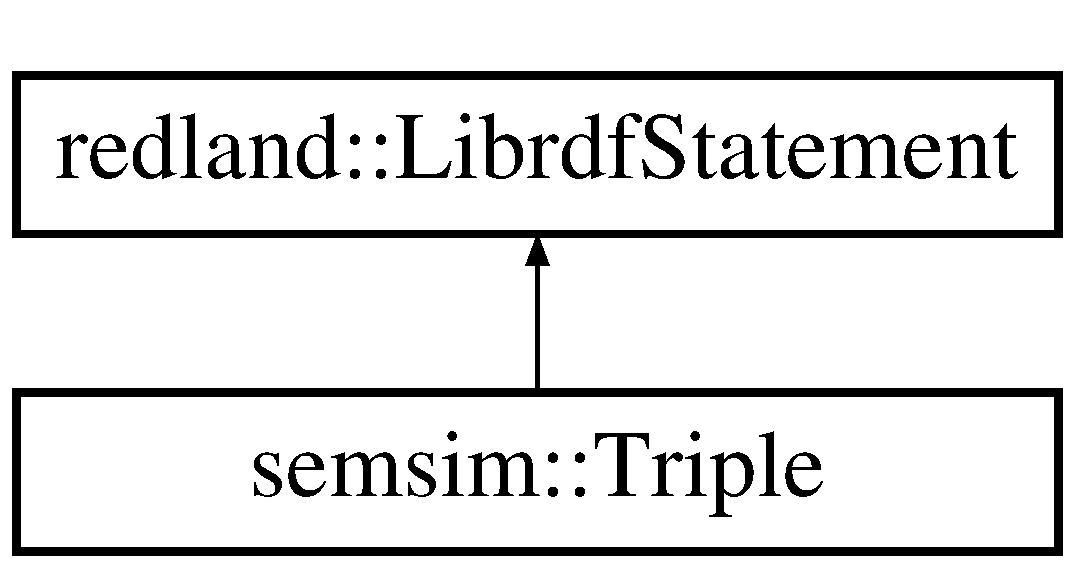
\includegraphics[height=2.000000cm]{classredland_1_1LibrdfStatement}
\end{center}
\end{figure}
\subsection*{Public Member Functions}
\begin{DoxyCompactItemize}
\item 
\mbox{\Hypertarget{classredland_1_1LibrdfStatement_ae7f7e27b7a502070195103268407243a}\label{classredland_1_1LibrdfStatement_ae7f7e27b7a502070195103268407243a}} 
{\bfseries Librdf\+Statement} (const \hyperlink{classredland_1_1LibrdfNode}{Librdf\+Node} \&subject, const \hyperlink{classredland_1_1LibrdfNode}{Librdf\+Node} \&predicate, const \hyperlink{classredland_1_1LibrdfNode}{Librdf\+Node} \&resource)
\item 
\mbox{\Hypertarget{classredland_1_1LibrdfStatement_a6b655a56f37dbe95fec840a0a1f0ed53}\label{classredland_1_1LibrdfStatement_a6b655a56f37dbe95fec840a0a1f0ed53}} 
librdf\+\_\+statement $\ast$ {\bfseries get} () const
\item 
\mbox{\Hypertarget{classredland_1_1LibrdfStatement_abcf022b8e24a74282e1d059fdf54d3fe}\label{classredland_1_1LibrdfStatement_abcf022b8e24a74282e1d059fdf54d3fe}} 
librdf\+\_\+node $\ast$ {\bfseries get\+Subject} () const
\item 
\mbox{\Hypertarget{classredland_1_1LibrdfStatement_a5aae51ac0994552a13f2c9b90bec63d0}\label{classredland_1_1LibrdfStatement_a5aae51ac0994552a13f2c9b90bec63d0}} 
librdf\+\_\+node $\ast$ {\bfseries get\+Predicate} () const
\item 
\mbox{\Hypertarget{classredland_1_1LibrdfStatement_aa763688f20b712ddc655afe405d7691a}\label{classredland_1_1LibrdfStatement_aa763688f20b712ddc655afe405d7691a}} 
librdf\+\_\+node $\ast$ {\bfseries get\+Resource} () const
\item 
\mbox{\Hypertarget{classredland_1_1LibrdfStatement_a6feed51cdebe7c4f2430fcba0ae17f37}\label{classredland_1_1LibrdfStatement_a6feed51cdebe7c4f2430fcba0ae17f37}} 
std\+::string {\bfseries get\+Subject\+Str} () const
\item 
\mbox{\Hypertarget{classredland_1_1LibrdfStatement_a5dd0d6a2e9fe1bfcf5254aa7928cdfaf}\label{classredland_1_1LibrdfStatement_a5dd0d6a2e9fe1bfcf5254aa7928cdfaf}} 
std\+::string {\bfseries get\+Predicate\+Str} () const
\item 
\mbox{\Hypertarget{classredland_1_1LibrdfStatement_adc21321df7ccf186c262e83a4438e993}\label{classredland_1_1LibrdfStatement_adc21321df7ccf186c262e83a4438e993}} 
std\+::string {\bfseries get\+Resource\+Str} () const
\item 
\mbox{\Hypertarget{classredland_1_1LibrdfStatement_a700219b2fed175a96fecfbd905d20ab1}\label{classredland_1_1LibrdfStatement_a700219b2fed175a96fecfbd905d20ab1}} 
void {\bfseries check\+For\+Null} ()
\item 
\mbox{\Hypertarget{classredland_1_1LibrdfStatement_a5fa27f77859a4673e991b9e86f84d889}\label{classredland_1_1LibrdfStatement_a5fa27f77859a4673e991b9e86f84d889}} 
void {\bfseries set\+Subject} (librdf\+\_\+node $\ast$node)
\item 
\mbox{\Hypertarget{classredland_1_1LibrdfStatement_a8b8fd2999e80bd2912af2430503a557a}\label{classredland_1_1LibrdfStatement_a8b8fd2999e80bd2912af2430503a557a}} 
void {\bfseries set\+Resource} (librdf\+\_\+node $\ast$node)
\item 
\mbox{\Hypertarget{classredland_1_1LibrdfStatement_a3306876fb080f3d19fca806142f93f87}\label{classredland_1_1LibrdfStatement_a3306876fb080f3d19fca806142f93f87}} 
void {\bfseries set\+Predicate} (librdf\+\_\+node $\ast$node)
\end{DoxyCompactItemize}
\subsection*{Static Public Member Functions}
\begin{DoxyCompactItemize}
\item 
\mbox{\Hypertarget{classredland_1_1LibrdfStatement_a9fb66c801d731ffce13e4d1381c49c29}\label{classredland_1_1LibrdfStatement_a9fb66c801d731ffce13e4d1381c49c29}} 
static \hyperlink{classredland_1_1LibrdfStatement}{Librdf\+Statement} {\bfseries from\+Raw\+Statement\+Ptr} (librdf\+\_\+statement $\ast$statement)
\item 
\mbox{\Hypertarget{classredland_1_1LibrdfStatement_a4eceaebc10deea27f4c75f7c8b4cccaf}\label{classredland_1_1LibrdfStatement_a4eceaebc10deea27f4c75f7c8b4cccaf}} 
static \hyperlink{classredland_1_1LibrdfStatement}{Librdf\+Statement} {\bfseries from\+Raw\+Node\+Ptrs} (librdf\+\_\+node $\ast$subject, librdf\+\_\+node $\ast$predicate, librdf\+\_\+node $\ast$resource)
\end{DoxyCompactItemize}
\subsection*{Protected Member Functions}
\begin{DoxyCompactItemize}
\item 
\mbox{\Hypertarget{classredland_1_1LibrdfStatement_afd63d6425b2130dbe4e76fdee4d7218b}\label{classredland_1_1LibrdfStatement_afd63d6425b2130dbe4e76fdee4d7218b}} 
void {\bfseries refresh\+Statement} ()
\item 
\mbox{\Hypertarget{classredland_1_1LibrdfStatement_a4cbbbf99d094cea4569324a8c67789fb}\label{classredland_1_1LibrdfStatement_a4cbbbf99d094cea4569324a8c67789fb}} 
{\bfseries Librdf\+Statement} (librdf\+\_\+statement $\ast$statement)
\item 
\mbox{\Hypertarget{classredland_1_1LibrdfStatement_ac1b38e67ff0b90ac54b27c4f5f5d9e12}\label{classredland_1_1LibrdfStatement_ac1b38e67ff0b90ac54b27c4f5f5d9e12}} 
{\bfseries Librdf\+Statement} (librdf\+\_\+node $\ast$subject, librdf\+\_\+node $\ast$predicate, librdf\+\_\+node $\ast$resource)
\end{DoxyCompactItemize}
\subsection*{Protected Attributes}
\begin{DoxyCompactItemize}
\item 
std\+::shared\+\_\+ptr$<$ librdf\+\_\+statement $>$ {\bfseries statement\+\_\+}
\end{DoxyCompactItemize}


\subsection{Member Data Documentation}
\mbox{\Hypertarget{classredland_1_1LibrdfStatement_ab76c572a450a69c9932a6f8534d978d5}\label{classredland_1_1LibrdfStatement_ab76c572a450a69c9932a6f8534d978d5}} 
\index{redland\+::\+Librdf\+Statement@{redland\+::\+Librdf\+Statement}!statement\+\_\+@{statement\+\_\+}}
\index{statement\+\_\+@{statement\+\_\+}!redland\+::\+Librdf\+Statement@{redland\+::\+Librdf\+Statement}}
\subsubsection{\texorpdfstring{statement\+\_\+}{statement\_}}
{\footnotesize\ttfamily std\+::shared\+\_\+ptr$<$librdf\+\_\+statement$>$ redland\+::\+Librdf\+Statement\+::statement\+\_\+\hspace{0.3cm}{\ttfamily [protected]}}

{\bfseries Initial value\+:}
\begin{DoxyCode}
= std::shared\_ptr<librdf\_statement>(
                librdf\_new\_statement(World::getWorld()),
                librdf\_free\_statement
        )
\end{DoxyCode}


The documentation for this class was generated from the following files\+:\begin{DoxyCompactItemize}
\item 
src/redland/\+Redland\+A\+P\+I\+Wrapper/src/Librdf\+Statement.\+h\item 
src/redland/\+Redland\+A\+P\+I\+Wrapper/src/Librdf\+Statement.\+cpp\end{DoxyCompactItemize}

\hypertarget{classredland_1_1LibrdfStorage}{}\section{redland\+:\+:Librdf\+Storage Class Reference}
\label{classredland_1_1LibrdfStorage}\index{redland\+::\+Librdf\+Storage@{redland\+::\+Librdf\+Storage}}
\subsection*{Public Member Functions}
\begin{DoxyCompactItemize}
\item 
\mbox{\Hypertarget{classredland_1_1LibrdfStorage_a8e3250af4dea528dcf94865835cfb8ff}\label{classredland_1_1LibrdfStorage_a8e3250af4dea528dcf94865835cfb8ff}} 
{\bfseries Librdf\+Storage} (librdf\+\_\+storage $\ast$storage)
\item 
\mbox{\Hypertarget{classredland_1_1LibrdfStorage_a08c025b165113efe1163c7294b989755}\label{classredland_1_1LibrdfStorage_a08c025b165113efe1163c7294b989755}} 
{\bfseries Librdf\+Storage} (const std\+::string \&storage\+\_\+name=\char`\"{}memory\char`\"{}, const std\+::string \&name=\char`\"{}Semsim\+Store\char`\"{}, const char $\ast$options=nullptr)
\item 
\mbox{\Hypertarget{classredland_1_1LibrdfStorage_a182d617ba7ab1b5359ef2693a56b272e}\label{classredland_1_1LibrdfStorage_a182d617ba7ab1b5359ef2693a56b272e}} 
librdf\+\_\+storage $\ast$ {\bfseries get} () const
\item 
\mbox{\Hypertarget{classredland_1_1LibrdfStorage_a7b08e7afd5ac5f38a0ed4cfeb77a3b99}\label{classredland_1_1LibrdfStorage_a7b08e7afd5ac5f38a0ed4cfeb77a3b99}} 
void {\bfseries free\+Storage} ()
\item 
\mbox{\Hypertarget{classredland_1_1LibrdfStorage_a7cef1518384fd6592ee8521cb95eb25d}\label{classredland_1_1LibrdfStorage_a7cef1518384fd6592ee8521cb95eb25d}} 
{\bfseries Librdf\+Storage} (const \hyperlink{classredland_1_1LibrdfStorage}{Librdf\+Storage} \&storage)=delete
\item 
\mbox{\Hypertarget{classredland_1_1LibrdfStorage_a59184a87b901f1d3709d045d57311606}\label{classredland_1_1LibrdfStorage_a59184a87b901f1d3709d045d57311606}} 
{\bfseries Librdf\+Storage} (\hyperlink{classredland_1_1LibrdfStorage}{Librdf\+Storage} \&\&storage) noexcept
\item 
\mbox{\Hypertarget{classredland_1_1LibrdfStorage_a1366716bbd3a0e41979d632c532c71ec}\label{classredland_1_1LibrdfStorage_a1366716bbd3a0e41979d632c532c71ec}} 
\hyperlink{classredland_1_1LibrdfStorage}{Librdf\+Storage} \& {\bfseries operator=} (\hyperlink{classredland_1_1LibrdfStorage}{Librdf\+Storage} \&\&storage) noexcept
\end{DoxyCompactItemize}


The documentation for this class was generated from the following files\+:\begin{DoxyCompactItemize}
\item 
src/redland/\+Redland\+A\+P\+I\+Wrapper/src/Librdf\+Storage.\+h\item 
src/redland/\+Redland\+A\+P\+I\+Wrapper/src/Librdf\+Storage.\+cpp\end{DoxyCompactItemize}

\hypertarget{classredland_1_1LibrdfStream}{}\section{redland\+:\+:Librdf\+Stream Class Reference}
\label{classredland_1_1LibrdfStream}\index{redland\+::\+Librdf\+Stream@{redland\+::\+Librdf\+Stream}}
\subsection*{Public Member Functions}
\begin{DoxyCompactItemize}
\item 
\mbox{\Hypertarget{classredland_1_1LibrdfStream_aaa64a7ef8a26be8cf35f3b31d6e34a1b}\label{classredland_1_1LibrdfStream_aaa64a7ef8a26be8cf35f3b31d6e34a1b}} 
{\bfseries Librdf\+Stream} (librdf\+\_\+stream $\ast$stream)
\item 
\mbox{\Hypertarget{classredland_1_1LibrdfStream_a5b52659abdfc01e583e1b9941eec2c4b}\label{classredland_1_1LibrdfStream_a5b52659abdfc01e583e1b9941eec2c4b}} 
librdf\+\_\+stream $\ast$ {\bfseries get} () const
\end{DoxyCompactItemize}


The documentation for this class was generated from the following files\+:\begin{DoxyCompactItemize}
\item 
src/redland/\+Redland\+A\+P\+I\+Wrapper/src/Librdf\+Stream.\+h\item 
src/redland/\+Redland\+A\+P\+I\+Wrapper/src/Librdf\+Stream.\+cpp\end{DoxyCompactItemize}

\hypertarget{classredland_1_1LibrdfUri}{}\section{redland\+:\+:Librdf\+Uri Class Reference}
\label{classredland_1_1LibrdfUri}\index{redland\+::\+Librdf\+Uri@{redland\+::\+Librdf\+Uri}}
\subsection*{Public Member Functions}
\begin{DoxyCompactItemize}
\item 
\mbox{\Hypertarget{classredland_1_1LibrdfUri_a3630cf904c9e4546fb6d6c175ed6c66e}\label{classredland_1_1LibrdfUri_a3630cf904c9e4546fb6d6c175ed6c66e}} 
\hyperlink{classredland_1_1LibrdfUri}{Librdf\+Uri} {\bfseries concatonate} (const std\+::string \&local\+\_\+name) const
\item 
\mbox{\Hypertarget{classredland_1_1LibrdfUri_acaeb8a0d4b6f493805ecc1b198807e1c}\label{classredland_1_1LibrdfUri_acaeb8a0d4b6f493805ecc1b198807e1c}} 
std\+::string {\bfseries str} () const
\item 
\mbox{\Hypertarget{classredland_1_1LibrdfUri_a36c5c589ae207ad6294e10be2bb8df17}\label{classredland_1_1LibrdfUri_a36c5c589ae207ad6294e10be2bb8df17}} 
{\bfseries Librdf\+Uri} (const std\+::string \&uri)
\item 
\mbox{\Hypertarget{classredland_1_1LibrdfUri_a1858bf7c3afae7d6d8ed2dca47e9cf55}\label{classredland_1_1LibrdfUri_a1858bf7c3afae7d6d8ed2dca47e9cf55}} 
librdf\+\_\+uri $\ast$ {\bfseries get} () const
\item 
\mbox{\Hypertarget{classredland_1_1LibrdfUri_ae9a8237bcb9cba0f2d87f2d980f579f3}\label{classredland_1_1LibrdfUri_ae9a8237bcb9cba0f2d87f2d980f579f3}} 
bool {\bfseries is\+Null} () const
\item 
\mbox{\Hypertarget{classredland_1_1LibrdfUri_a13f1a7bc775cd79b6bb4dc6cd31b5d53}\label{classredland_1_1LibrdfUri_a13f1a7bc775cd79b6bb4dc6cd31b5d53}} 
bool {\bfseries is\+Empty} () const
\item 
\mbox{\Hypertarget{classredland_1_1LibrdfUri_aa07e6315dc3428b6d864deb00cda48e1}\label{classredland_1_1LibrdfUri_aa07e6315dc3428b6d864deb00cda48e1}} 
void {\bfseries free\+Uri} ()
\item 
\mbox{\Hypertarget{classredland_1_1LibrdfUri_a770d47b63c041e39761f8dd46b0bf8b5}\label{classredland_1_1LibrdfUri_a770d47b63c041e39761f8dd46b0bf8b5}} 
bool {\bfseries is\+File\+Uri} () const
\item 
\mbox{\Hypertarget{classredland_1_1LibrdfUri_a02d802c21de7c9dba4133779701e3a45}\label{classredland_1_1LibrdfUri_a02d802c21de7c9dba4133779701e3a45}} 
bool {\bfseries operator==} (const \hyperlink{classredland_1_1LibrdfUri}{Librdf\+Uri} \&rhs) const
\item 
\mbox{\Hypertarget{classredland_1_1LibrdfUri_a8ded118526be9cfdbe6dbc87d075fb06}\label{classredland_1_1LibrdfUri_a8ded118526be9cfdbe6dbc87d075fb06}} 
bool {\bfseries operator!=} (const \hyperlink{classredland_1_1LibrdfUri}{Librdf\+Uri} \&rhs) const
\item 
\mbox{\Hypertarget{classredland_1_1LibrdfUri_ad24448f9b22adce080a35decc4694479}\label{classredland_1_1LibrdfUri_ad24448f9b22adce080a35decc4694479}} 
std\+::string {\bfseries to\+Filename\+String} () const
\end{DoxyCompactItemize}
\subsection*{Static Public Member Functions}
\begin{DoxyCompactItemize}
\item 
\mbox{\Hypertarget{classredland_1_1LibrdfUri_a518761e1fbfd8c2f79dcac01b05c720b}\label{classredland_1_1LibrdfUri_a518761e1fbfd8c2f79dcac01b05c720b}} 
static \hyperlink{classredland_1_1LibrdfUri}{Librdf\+Uri} {\bfseries from\+Raw\+Ptr} (librdf\+\_\+uri $\ast$uri)
\item 
\mbox{\Hypertarget{classredland_1_1LibrdfUri_ad7245bf32a2538d220ec7d3a0afc0802}\label{classredland_1_1LibrdfUri_ad7245bf32a2538d220ec7d3a0afc0802}} 
static \hyperlink{classredland_1_1LibrdfUri}{Librdf\+Uri} {\bfseries from\+Filename} (const std\+::string \&filename)
\item 
\mbox{\Hypertarget{classredland_1_1LibrdfUri_a58ab2ce202cc9b563d1dc60a20a545b2}\label{classredland_1_1LibrdfUri_a58ab2ce202cc9b563d1dc60a20a545b2}} 
static \hyperlink{classredland_1_1LibrdfUri}{Librdf\+Uri} {\bfseries concatonate} (librdf\+\_\+uri $\ast$old\+\_\+name, const std\+::string \&local\+\_\+name)
\end{DoxyCompactItemize}


The documentation for this class was generated from the following files\+:\begin{DoxyCompactItemize}
\item 
src/redland/\+Redland\+A\+P\+I\+Wrapper/src/Librdf\+Uri.\+h\item 
src/redland/\+Redland\+A\+P\+I\+Wrapper/src/Librdf\+Uri.\+cpp\end{DoxyCompactItemize}

\hypertarget{classsemsim_1_1MediatorParticipant}{}\doxysection{semsim\+::Mediator\+Participant Class Reference}
\label{classsemsim_1_1MediatorParticipant}\index{semsim::MediatorParticipant@{semsim::MediatorParticipant}}
Inheritance diagram for semsim\+::Mediator\+Participant\+:\begin{figure}[H]
                                                              \begin{center}
                                                                  \leavevmode
                                                                  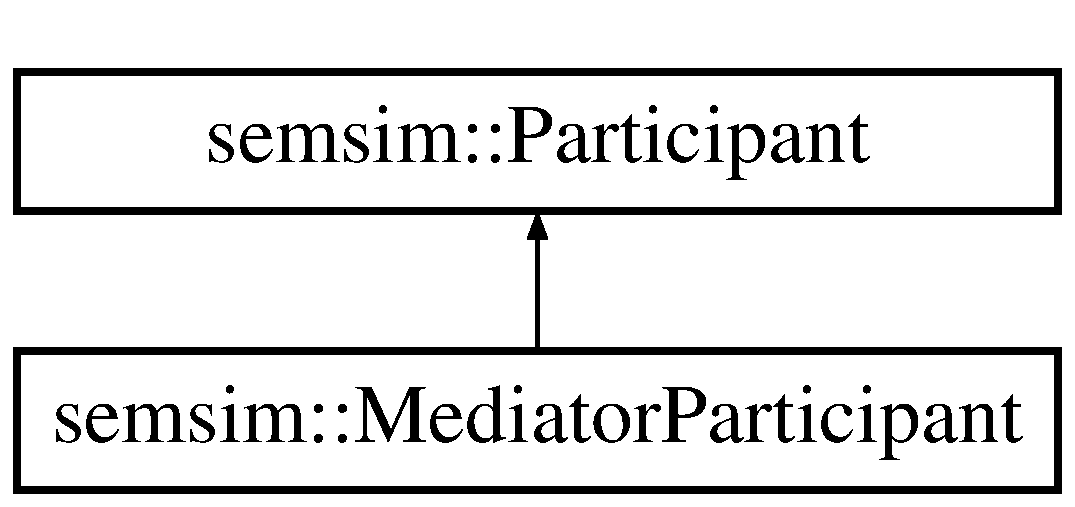
\includegraphics[height=2.000000cm]{classsemsim_1_1MediatorParticipant}
                                                              \end{center}
\end{figure}
\doxysubsection*{Public Member Functions}
\begin{DoxyCompactItemize}
    \item
    \mbox{\Hypertarget{classsemsim_1_1MediatorParticipant_a068e325880c96b598b5ea87edcaffcd4}\label{classsemsim_1_1MediatorParticipant_a068e325880c96b598b5ea87edcaffcd4}}
    {\bfseries Mediator\+Participant} (Librdf\+World world, Librdf\+Model model, std\+::string subject, std\+::string physical\+Entity\+Reference)
\end{DoxyCompactItemize}


The documentation for this class was generated from the following files\+:\begin{DoxyCompactItemize}
                                                                              \item
                                                                              src/semsim/Participant.\+h\item
                                                                              src/semsim/Participant.\+cpp
\end{DoxyCompactItemize}

\hypertarget{classsemsim_1_1MetaID}{}\section{semsim\+:\+:Meta\+ID Class Reference}
\label{classsemsim_1_1MetaID}\index{semsim\+::\+Meta\+ID@{semsim\+::\+Meta\+ID}}
\subsection*{Public Member Functions}
\begin{DoxyCompactItemize}
\item 
\mbox{\Hypertarget{classsemsim_1_1MetaID_a63833c9ae3303f451181f9d118c0d51c}\label{classsemsim_1_1MetaID_a63833c9ae3303f451181f9d118c0d51c}} 
{\bfseries Meta\+ID} (std\+::string base, long number, int num\+\_\+digits=4)
\item 
\mbox{\Hypertarget{classsemsim_1_1MetaID_a4b39fce25e5db81fdd59cfbc4f4734da}\label{classsemsim_1_1MetaID_a4b39fce25e5db81fdd59cfbc4f4734da}} 
bool {\bfseries operator==} (const \hyperlink{classsemsim_1_1MetaID}{Meta\+ID} \&rhs) const
\item 
\mbox{\Hypertarget{classsemsim_1_1MetaID_a128d53d2d266cf1f88ef13ee9c21a2c0}\label{classsemsim_1_1MetaID_a128d53d2d266cf1f88ef13ee9c21a2c0}} 
bool {\bfseries operator!=} (const \hyperlink{classsemsim_1_1MetaID}{Meta\+ID} \&rhs) const
\item 
\mbox{\Hypertarget{classsemsim_1_1MetaID_aefd0d224e3930da32f927a4ff8c8bc74}\label{classsemsim_1_1MetaID_aefd0d224e3930da32f927a4ff8c8bc74}} 
std\+::string {\bfseries generate} () const
\item 
\mbox{\Hypertarget{classsemsim_1_1MetaID_a6336339cef2d12f7eea49bab94e45171}\label{classsemsim_1_1MetaID_a6336339cef2d12f7eea49bab94e45171}} 
std\+::string {\bfseries generate} (long n) const
\item 
\mbox{\Hypertarget{classsemsim_1_1MetaID_a2a9408d835ed445a90b43843404e9fbe}\label{classsemsim_1_1MetaID_a2a9408d835ed445a90b43843404e9fbe}} 
int {\bfseries max\+Number} () const
\end{DoxyCompactItemize}
\subsection*{Static Public Member Functions}
\begin{DoxyCompactItemize}
\item 
\mbox{\Hypertarget{classsemsim_1_1MetaID_aa4f326f8b965d3dd7af038793e7806ad}\label{classsemsim_1_1MetaID_aa4f326f8b965d3dd7af038793e7806ad}} 
static int {\bfseries count\+Digits} (long n)
\end{DoxyCompactItemize}


The documentation for this class was generated from the following files\+:\begin{DoxyCompactItemize}
\item 
src/semsim/Meta\+I\+D.\+h\item 
src/semsim/Meta\+I\+D.\+cpp\end{DoxyCompactItemize}

\hypertarget{classsemsim_1_1NotImplementedException}{}\doxysection{semsim\+::Not\+Implemented\+Exception Class Reference}
\label{classsemsim_1_1NotImplementedException}\index{semsim::NotImplementedException@{semsim::NotImplementedException}}
Inheritance diagram for semsim\+::Not\+Implemented\+Exception\+:\begin{figure}[H]
                                                                    \begin{center}
                                                                        \leavevmode
                                                                        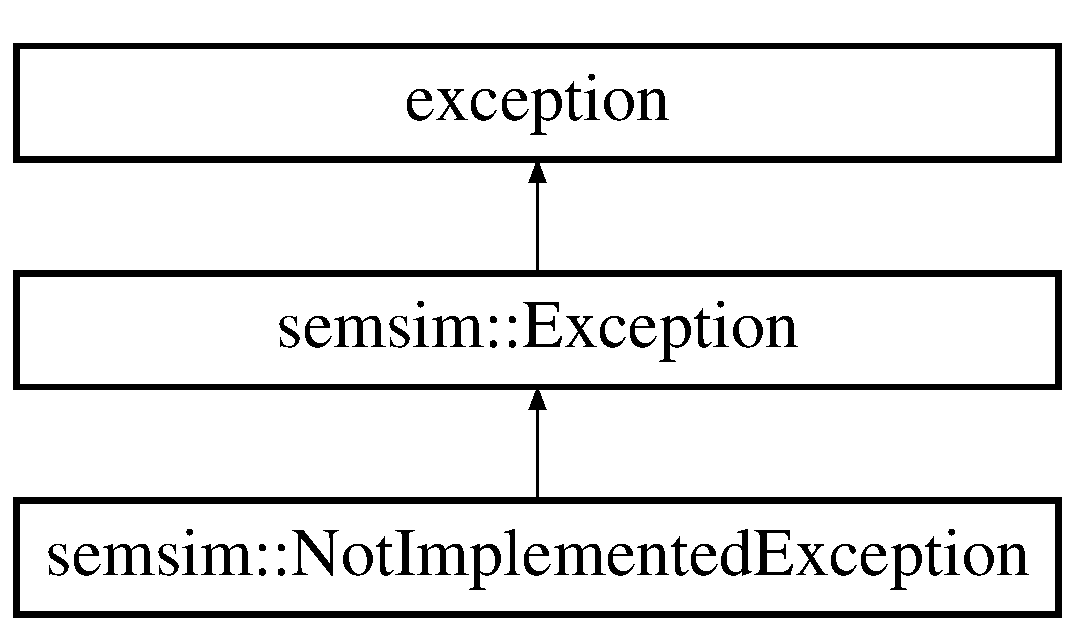
\includegraphics[height=3.000000cm]{classsemsim_1_1NotImplementedException}
                                                                    \end{center}
\end{figure}
\doxysubsection*{Additional Inherited Members}


The documentation for this class was generated from the following file\+:\begin{DoxyCompactItemize}
                                                                             \item
                                                                             src/semsim/Error.\+h
\end{DoxyCompactItemize}

\hypertarget{classsemsim_1_1NullPointerException}{}\doxysection{semsim\+::Null\+Pointer\+Exception Class Reference}
\label{classsemsim_1_1NullPointerException}\index{semsim::NullPointerException@{semsim::NullPointerException}}
Inheritance diagram for semsim\+::Null\+Pointer\+Exception\+:\begin{figure}[H]
                                                                 \begin{center}
                                                                     \leavevmode
                                                                     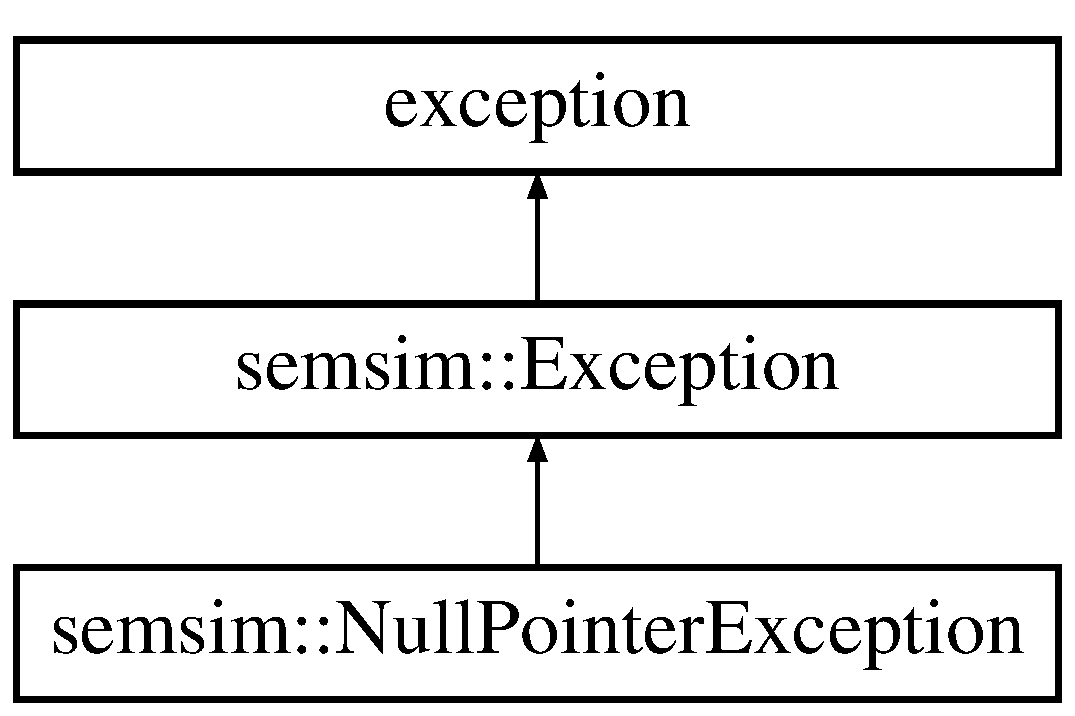
\includegraphics[height=3.000000cm]{classsemsim_1_1NullPointerException}
                                                                 \end{center}
\end{figure}
\doxysubsection*{Additional Inherited Members}


The documentation for this class was generated from the following file\+:\begin{DoxyCompactItemize}
                                                                             \item
                                                                             src/semsim/Error.\+h
\end{DoxyCompactItemize}

\hypertarget{classsemsim_1_1Participant}{}\doxysection{semsim\+::Participant Class Reference}
\label{classsemsim_1_1Participant}\index{semsim::Participant@{semsim::Participant}}
Inheritance diagram for semsim\+::Participant\+:\begin{figure}[H]
                                                    \begin{center}
                                                        \leavevmode
                                                        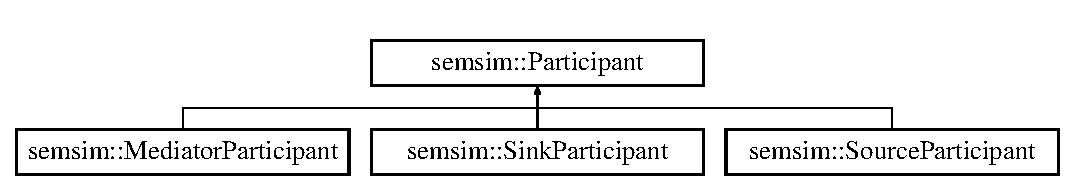
\includegraphics[height=2.000000cm]{classsemsim_1_1Participant}
                                                    \end{center}
\end{figure}
\doxysubsection*{Public Member Functions}
\begin{DoxyCompactItemize}
    \item
    \mbox{\Hypertarget{classsemsim_1_1Participant_a3d88edb6809ef1339681325820cc6f68}\label{classsemsim_1_1Participant_a3d88edb6809ef1339681325820cc6f68}}
    {\bfseries Participant} (Librdf\+World world, Librdf\+Model model, std\+::string subject, Predicate\+Ptr predicate, double multiplier, std\+::string physical\+Entity\+Reference)
    \item
    \mbox{\Hypertarget{classsemsim_1_1Participant_af2096dc5c0657d3c6a704ec6111bf063}\label{classsemsim_1_1Participant_af2096dc5c0657d3c6a704ec6111bf063}}
    \mbox{\hyperlink{classsemsim_1_1Triples}{Triples}} {\bfseries to\+Triples} (std\+::string process\+\_\+metaid) const
    \item
    \mbox{\Hypertarget{classsemsim_1_1Participant_a64bdbfd4784ea280c9349e8f54ebff0a}\label{classsemsim_1_1Participant_a64bdbfd4784ea280c9349e8f54ebff0a}}
    Predicate\+Ptr {\bfseries get\+Predicate\+Ptr} ()
    \item
    \mbox{\Hypertarget{classsemsim_1_1Participant_aa8fc565de215a712a23f65d0a004a041}\label{classsemsim_1_1Participant_aa8fc565de215a712a23f65d0a004a041}}
    void {\bfseries set\+Predicate\+Ptr} (Predicate\+Ptr predicate\+\_\+ptr)
    \item
    \mbox{\Hypertarget{classsemsim_1_1Participant_a4558e59757e79df410554b920a354bb6}\label{classsemsim_1_1Participant_a4558e59757e79df410554b920a354bb6}}
    Librdf\+World {\bfseries get\+World} () const
    \item
    \mbox{\Hypertarget{classsemsim_1_1Participant_acfdc8056b288b3e36d54248d03d96c5c}\label{classsemsim_1_1Participant_acfdc8056b288b3e36d54248d03d96c5c}}
    const std\+::string \& {\bfseries get\+Subject} () const
    \item
    \mbox{\Hypertarget{classsemsim_1_1Participant_aca088588f5fa41042be8cc43ceeb7962}\label{classsemsim_1_1Participant_aca088588f5fa41042be8cc43ceeb7962}}
    double {\bfseries get\+Multiplier} () const
    \item
    \mbox{\Hypertarget{classsemsim_1_1Participant_a7c9e14ea7bc01d2fc6b655a990b370f3}\label{classsemsim_1_1Participant_a7c9e14ea7bc01d2fc6b655a990b370f3}}
    const std\+::string \& {\bfseries get\+Physical\+Entity\+Reference} () const
\end{DoxyCompactItemize}


The documentation for this class was generated from the following files\+:\begin{DoxyCompactItemize}
                                                                              \item
                                                                              src/semsim/Participant.\+h\item
                                                                              src/semsim/Participant.\+cpp
\end{DoxyCompactItemize}

\hypertarget{classsemsim_1_1PhysicalEntity}{}\section{semsim\+:\+:Physical\+Entity Class Reference}
\label{classsemsim_1_1PhysicalEntity}\index{semsim\+::\+Physical\+Entity@{semsim\+::\+Physical\+Entity}}
Inheritance diagram for semsim\+:\+:Physical\+Entity\+:\begin{figure}[H]
\begin{center}
\leavevmode
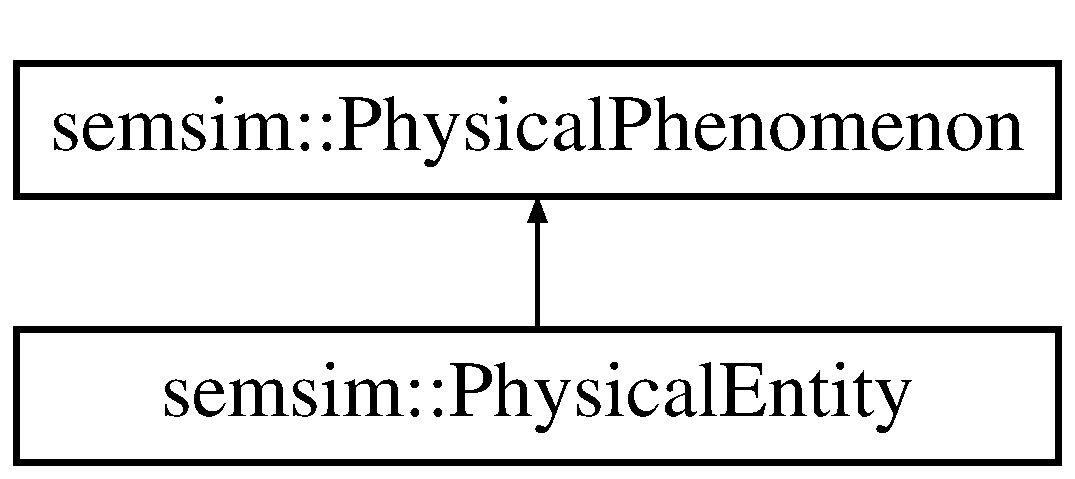
\includegraphics[height=2.000000cm]{classsemsim_1_1PhysicalEntity}
\end{center}
\end{figure}
\subsection*{Public Member Functions}
\begin{DoxyCompactItemize}
\item 
\mbox{\Hypertarget{classsemsim_1_1PhysicalEntity_a38bf3915fbd86b2adb9e9779301a94b3}\label{classsemsim_1_1PhysicalEntity_a38bf3915fbd86b2adb9e9779301a94b3}} 
{\bfseries Physical\+Entity} (librdf\+\_\+model $\ast$model, \hyperlink{classsemsim_1_1Subject}{Subject} about, \hyperlink{classsemsim_1_1PhysicalPropertyResource}{Physical\+Property\+Resource} physical\+Property, \hyperlink{classsemsim_1_1Resource}{Resource} is, Resources is\+\_\+part\+\_\+of)
\item 
\mbox{\Hypertarget{classsemsim_1_1PhysicalEntity_a3978fc7ce8633d583965a858ee99a418}\label{classsemsim_1_1PhysicalEntity_a3978fc7ce8633d583965a858ee99a418}} 
void {\bfseries free} () override
\item 
\mbox{\Hypertarget{classsemsim_1_1PhysicalEntity_a1df028fe0ee3f7f58e2eb7ea28d118ec}\label{classsemsim_1_1PhysicalEntity_a1df028fe0ee3f7f58e2eb7ea28d118ec}} 
{\bfseries Physical\+Entity} (librdf\+\_\+model $\ast$model)
\item 
\mbox{\Hypertarget{classsemsim_1_1PhysicalEntity_a32f4240e1ab47f422e704f97c669e824}\label{classsemsim_1_1PhysicalEntity_a32f4240e1ab47f422e704f97c669e824}} 
\hyperlink{classsemsim_1_1Triples}{Triples} {\bfseries to\+Triples} () override
\item 
\mbox{\Hypertarget{classsemsim_1_1PhysicalEntity_a5940a4984dbd8fb6cef55de5cd36a9b4}\label{classsemsim_1_1PhysicalEntity_a5940a4984dbd8fb6cef55de5cd36a9b4}} 
const \hyperlink{classsemsim_1_1Resource}{Resource} \& {\bfseries get\+Identity\+Resource} () const
\item 
\mbox{\Hypertarget{classsemsim_1_1PhysicalEntity_aa2aeec22fc0f703b2e83fcfd59b25f29}\label{classsemsim_1_1PhysicalEntity_aa2aeec22fc0f703b2e83fcfd59b25f29}} 
const Resources \& {\bfseries get\+Location\+Resources} () const
\item 
\mbox{\Hypertarget{classsemsim_1_1PhysicalEntity_aa5b88988a264a59b174452ec49f824ba}\label{classsemsim_1_1PhysicalEntity_aa5b88988a264a59b174452ec49f824ba}} 
\hyperlink{classsemsim_1_1PhysicalEntity}{Physical\+Entity} \& {\bfseries set\+About} (std\+::string metaid)
\item 
\mbox{\Hypertarget{classsemsim_1_1PhysicalEntity_ae2408ca531d0755ff28ad1e4f062023d}\label{classsemsim_1_1PhysicalEntity_ae2408ca531d0755ff28ad1e4f062023d}} 
\hyperlink{classsemsim_1_1PhysicalEntity}{Physical\+Entity} \& {\bfseries set\+Physical\+Property} (const std\+::string \&physical\+Property)
\item 
\mbox{\Hypertarget{classsemsim_1_1PhysicalEntity_a4aa4c32d99568eb43ec97d8371ded354}\label{classsemsim_1_1PhysicalEntity_a4aa4c32d99568eb43ec97d8371ded354}} 
\hyperlink{classsemsim_1_1PhysicalEntity}{Physical\+Entity} \& {\bfseries set\+Physical\+Property} (\hyperlink{classsemsim_1_1PhysicalPropertyResource}{Physical\+Property\+Resource} physical\+Property)
\item 
\mbox{\Hypertarget{classsemsim_1_1PhysicalEntity_ab3e7a2142a90e18150323268acc92217}\label{classsemsim_1_1PhysicalEntity_ab3e7a2142a90e18150323268acc92217}} 
\hyperlink{classsemsim_1_1PhysicalEntity}{Physical\+Entity} \& {\bfseries set\+Identity} (std\+::string resource)
\item 
\mbox{\Hypertarget{classsemsim_1_1PhysicalEntity_a1b35c526b4265b920d9d483842e0150d}\label{classsemsim_1_1PhysicalEntity_a1b35c526b4265b920d9d483842e0150d}} 
\hyperlink{classsemsim_1_1PhysicalEntity}{Physical\+Entity} \& {\bfseries add\+Location} (std\+::string where)
\item 
\mbox{\Hypertarget{classsemsim_1_1PhysicalEntity_a8db27f0206e3d827f5b8866459a771aa}\label{classsemsim_1_1PhysicalEntity_a8db27f0206e3d827f5b8866459a771aa}} 
int {\bfseries get\+Num\+Locations} () const
\end{DoxyCompactItemize}
\subsection*{Additional Inherited Members}


The documentation for this class was generated from the following files\+:\begin{DoxyCompactItemize}
\item 
src/semsim/Physical\+Entity.\+h\item 
src/semsim/Physical\+Entity.\+cpp\end{DoxyCompactItemize}

\hypertarget{classsemsim_1_1PhysicalForce}{}\section{semsim\+:\+:Physical\+Force Class Reference}
\label{classsemsim_1_1PhysicalForce}\index{semsim\+::\+Physical\+Force@{semsim\+::\+Physical\+Force}}
Inheritance diagram for semsim\+:\+:Physical\+Force\+:\begin{figure}[H]
\begin{center}
\leavevmode
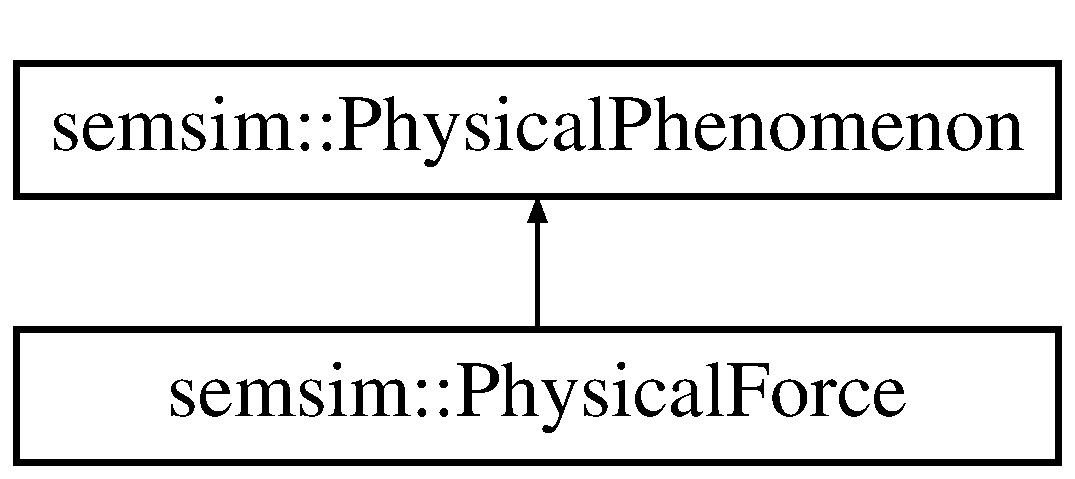
\includegraphics[height=2.000000cm]{classsemsim_1_1PhysicalForce}
\end{center}
\end{figure}
\subsection*{Public Member Functions}
\begin{DoxyCompactItemize}
\item 
\mbox{\Hypertarget{classsemsim_1_1PhysicalForce_ab4a55fec692b38b868ddd357f82969bd}\label{classsemsim_1_1PhysicalForce_ab4a55fec692b38b868ddd357f82969bd}} 
{\bfseries Physical\+Force} (librdf\+\_\+model $\ast$model, \hyperlink{classsemsim_1_1Subject}{Subject} metaid, \hyperlink{classsemsim_1_1PhysicalPropertyResource}{Physical\+Property\+Resource} physical\+Property, Sources sources, Sinks sinks)
\item 
\mbox{\Hypertarget{classsemsim_1_1PhysicalForce_a5d5a07e0f6d88cd5569c78a6039f3de1}\label{classsemsim_1_1PhysicalForce_a5d5a07e0f6d88cd5569c78a6039f3de1}} 
void {\bfseries free} () override
\item 
\mbox{\Hypertarget{classsemsim_1_1PhysicalForce_a08cf520fbe7955eca7766b9d2c5bc0c8}\label{classsemsim_1_1PhysicalForce_a08cf520fbe7955eca7766b9d2c5bc0c8}} 
{\bfseries Physical\+Force} (librdf\+\_\+model $\ast$model)
\item 
\mbox{\Hypertarget{classsemsim_1_1PhysicalForce_a740ffadd18b39ce922b41633db3e24af}\label{classsemsim_1_1PhysicalForce_a740ffadd18b39ce922b41633db3e24af}} 
std\+::string {\bfseries create\+Meta\+Id} () const
\item 
\mbox{\Hypertarget{classsemsim_1_1PhysicalForce_a3641e487b723088a5ecf82488877cc34}\label{classsemsim_1_1PhysicalForce_a3641e487b723088a5ecf82488877cc34}} 
const Sources \& {\bfseries get\+Sources} () const
\item 
\mbox{\Hypertarget{classsemsim_1_1PhysicalForce_a5ca80b2444abf551937c7864abea4980}\label{classsemsim_1_1PhysicalForce_a5ca80b2444abf551937c7864abea4980}} 
const Sinks \& {\bfseries get\+Sinks} () const
\item 
\mbox{\Hypertarget{classsemsim_1_1PhysicalForce_a9b8be504b403b781a34ca5df9c3bbc2d}\label{classsemsim_1_1PhysicalForce_a9b8be504b403b781a34ca5df9c3bbc2d}} 
\hyperlink{classsemsim_1_1Triples}{Triples} {\bfseries to\+Triples} () override
\item 
\mbox{\Hypertarget{classsemsim_1_1PhysicalForce_ad817f08d345b53a2e7fb80052457f8c8}\label{classsemsim_1_1PhysicalForce_ad817f08d345b53a2e7fb80052457f8c8}} 
\hyperlink{classsemsim_1_1PhysicalForce}{Physical\+Force} \& {\bfseries set\+About} (const std\+::string \&metaid)
\item 
\mbox{\Hypertarget{classsemsim_1_1PhysicalForce_a5a83ae2458a89151ed7990ba75251318}\label{classsemsim_1_1PhysicalForce_a5a83ae2458a89151ed7990ba75251318}} 
\hyperlink{classsemsim_1_1PhysicalForce}{Physical\+Force} \& {\bfseries set\+Physical\+Property} (\hyperlink{classsemsim_1_1PhysicalPropertyResource}{Physical\+Property\+Resource} physical\+Property)
\item 
\mbox{\Hypertarget{classsemsim_1_1PhysicalForce_a684767a1350eab54b403c5b1dd0cb20a}\label{classsemsim_1_1PhysicalForce_a684767a1350eab54b403c5b1dd0cb20a}} 
\hyperlink{classsemsim_1_1PhysicalForce}{Physical\+Force} \& {\bfseries set\+Physical\+Property} (const std\+::string \&physical\+Property)
\item 
\mbox{\Hypertarget{classsemsim_1_1PhysicalForce_afe234b09ac757b4cf3561f8d3cbf4c0b}\label{classsemsim_1_1PhysicalForce_afe234b09ac757b4cf3561f8d3cbf4c0b}} 
\hyperlink{classsemsim_1_1PhysicalForce}{Physical\+Force} \& {\bfseries add\+Source} (std\+::string source\+\_\+metaid, double multiplier, std\+::string physical\+\_\+entity\+\_\+reference)
\item 
\mbox{\Hypertarget{classsemsim_1_1PhysicalForce_a0886647a9a7efd80bb99f6ce74bcb76a}\label{classsemsim_1_1PhysicalForce_a0886647a9a7efd80bb99f6ce74bcb76a}} 
\hyperlink{classsemsim_1_1PhysicalForce}{Physical\+Force} \& {\bfseries add\+Sink} (std\+::string sink\+\_\+metaid, double multiplier, std\+::string physical\+\_\+entity\+\_\+reference)
\item 
\mbox{\Hypertarget{classsemsim_1_1PhysicalForce_ad94974c799d17e5f6376391b1f3a7444}\label{classsemsim_1_1PhysicalForce_ad94974c799d17e5f6376391b1f3a7444}} 
int {\bfseries get\+Num\+Sources} ()
\item 
\mbox{\Hypertarget{classsemsim_1_1PhysicalForce_ab947284af190941616ae8a6f1de2a85d}\label{classsemsim_1_1PhysicalForce_ab947284af190941616ae8a6f1de2a85d}} 
int {\bfseries get\+Num\+Sinks} ()
\end{DoxyCompactItemize}
\subsection*{Additional Inherited Members}


The documentation for this class was generated from the following files\+:\begin{DoxyCompactItemize}
\item 
src/semsim/Physical\+Force.\+h\item 
src/semsim/Physical\+Force.\+cpp\end{DoxyCompactItemize}

\hypertarget{classsemsim_1_1PhysicalPhenomenon}{}\doxysection{semsim\+::Physical\+Phenomenon Class Reference}
\label{classsemsim_1_1PhysicalPhenomenon}\index{semsim::PhysicalPhenomenon@{semsim::PhysicalPhenomenon}}
Inheritance diagram for semsim\+::Physical\+Phenomenon\+:\begin{figure}[H]
                                                             \begin{center}
                                                                 \leavevmode
                                                                 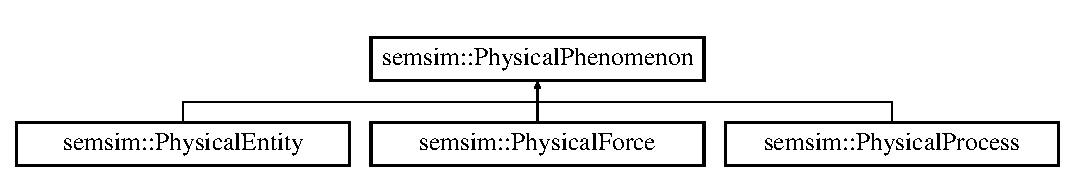
\includegraphics[height=1.996435cm]{classsemsim_1_1PhysicalPhenomenon}
                                                             \end{center}
\end{figure}
\doxysubsection*{Public Member Functions}
\begin{DoxyCompactItemize}
    \item
    \mbox{\Hypertarget{classsemsim_1_1PhysicalPhenomenon_a4923938fde324d41d9d2d171c380d512}\label{classsemsim_1_1PhysicalPhenomenon_a4923938fde324d41d9d2d171c380d512}}
    {\bfseries Physical\+Phenomenon} (Librdf\+World world, Librdf\+Model model, \mbox{\hyperlink{classsemsim_1_1Subject}{Subject}} metaid, \mbox{\hyperlink{classsemsim_1_1PhysicalPropertyResource}{Physical\+Property\+Resource}} property\+Resource, Annotation\+Type type)
    \item
    \mbox{\Hypertarget{classsemsim_1_1PhysicalPhenomenon_a7d148d741a60a8384e596b9902d5675d}\label{classsemsim_1_1PhysicalPhenomenon_a7d148d741a60a8384e596b9902d5675d}}
    {\bfseries Physical\+Phenomenon} (Librdf\+World world, Librdf\+Model model)
    \item
    \mbox{\Hypertarget{classsemsim_1_1PhysicalPhenomenon_af3a680b3bacba8733eab51207fa8e223}\label{classsemsim_1_1PhysicalPhenomenon_af3a680b3bacba8733eab51207fa8e223}}
    \mbox{\hyperlink{classsemsim_1_1Subject}{Subject}} {\bfseries get\+About} () const
    \item
    \mbox{\Hypertarget{classsemsim_1_1PhysicalPhenomenon_ae56630b175214b2196da1bf47a3c47c0}\label{classsemsim_1_1PhysicalPhenomenon_ae56630b175214b2196da1bf47a3c47c0}}
    \mbox{\hyperlink{classsemsim_1_1Subject}{Subject}} {\bfseries get\+Subject} () const
    \item
    \mbox{\Hypertarget{classsemsim_1_1PhysicalPhenomenon_a3fc27dfe9bedd3055c575e134c537d6e}\label{classsemsim_1_1PhysicalPhenomenon_a3fc27dfe9bedd3055c575e134c537d6e}}
    Annotation\+Type {\bfseries get\+Type} () const
    \item
    \mbox{\Hypertarget{classsemsim_1_1PhysicalPhenomenon_ac0b9bb899a6bd02275b5b4d106f875ea}\label{classsemsim_1_1PhysicalPhenomenon_ac0b9bb899a6bd02275b5b4d106f875ea}}
    \mbox{\hyperlink{classsemsim_1_1PhysicalPropertyResource}{Physical\+Property\+Resource}} {\bfseries get\+Physical\+Property} () const
    \item
    \mbox{\Hypertarget{classsemsim_1_1PhysicalPhenomenon_a1856c2c2c86e053d8b164f401810f308}\label{classsemsim_1_1PhysicalPhenomenon_a1856c2c2c86e053d8b164f401810f308}}
    virtual \mbox{\hyperlink{classsemsim_1_1Triples}{Triples}} {\bfseries to\+Triples} () const
\end{DoxyCompactItemize}
\doxysubsection*{Protected Member Functions}
\begin{DoxyCompactItemize}
    \item
    \mbox{\Hypertarget{classsemsim_1_1PhysicalPhenomenon_a930e9d0f75ec3a7bdbcb2dbce1a47716}\label{classsemsim_1_1PhysicalPhenomenon_a930e9d0f75ec3a7bdbcb2dbce1a47716}}
    std\+::string {\bfseries generate\+Meta\+Id} (std\+::string id\+\_\+base) const
\end{DoxyCompactItemize}
\doxysubsection*{Protected Attributes}
\begin{DoxyCompactItemize}
    \item
    \mbox{\Hypertarget{classsemsim_1_1PhysicalPhenomenon_a6352d5bc90b9050b6b8eda6f5691d0a3}\label{classsemsim_1_1PhysicalPhenomenon_a6352d5bc90b9050b6b8eda6f5691d0a3}}
    Librdf\+World {\bfseries world\+\_\+}
    \item
    \mbox{\Hypertarget{classsemsim_1_1PhysicalPhenomenon_ae90491b509bf2c7d7b604804fc1b34e5}\label{classsemsim_1_1PhysicalPhenomenon_ae90491b509bf2c7d7b604804fc1b34e5}}
    Librdf\+Model {\bfseries model\+\_\+}
    \item
    \mbox{\Hypertarget{classsemsim_1_1PhysicalPhenomenon_aa43a5f6719a6d44d4b96081b2f2622fe}\label{classsemsim_1_1PhysicalPhenomenon_aa43a5f6719a6d44d4b96081b2f2622fe}}
    \mbox{\hyperlink{classsemsim_1_1Subject}{Subject}} {\bfseries about}
    \item
    \mbox{\Hypertarget{classsemsim_1_1PhysicalPhenomenon_a264d752c356d2c6011da6d3cd1494418}\label{classsemsim_1_1PhysicalPhenomenon_a264d752c356d2c6011da6d3cd1494418}}
    \mbox{\hyperlink{classsemsim_1_1PhysicalPropertyResource}{Physical\+Property\+Resource}} {\bfseries physical\+\_\+property\+\_\+}
    \item
    \mbox{\Hypertarget{classsemsim_1_1PhysicalPhenomenon_ad18e38168bcec1925e6bd9ed08494614}\label{classsemsim_1_1PhysicalPhenomenon_ad18e38168bcec1925e6bd9ed08494614}}
    Annotation\+Type {\bfseries type\+\_\+}
\end{DoxyCompactItemize}


The documentation for this class was generated from the following files\+:\begin{DoxyCompactItemize}
                                                                              \item
                                                                              src/semsim/Physical\+Phenomenon.\+h\item
                                                                              src/semsim/Physical\+Phenomenon.\+cpp
\end{DoxyCompactItemize}

\hypertarget{classsemsim_1_1PhysicalProcess}{}\section{semsim\+:\+:Physical\+Process Class Reference}
\label{classsemsim_1_1PhysicalProcess}\index{semsim\+::\+Physical\+Process@{semsim\+::\+Physical\+Process}}
Inheritance diagram for semsim\+:\+:Physical\+Process\+:\begin{figure}[H]
\begin{center}
\leavevmode
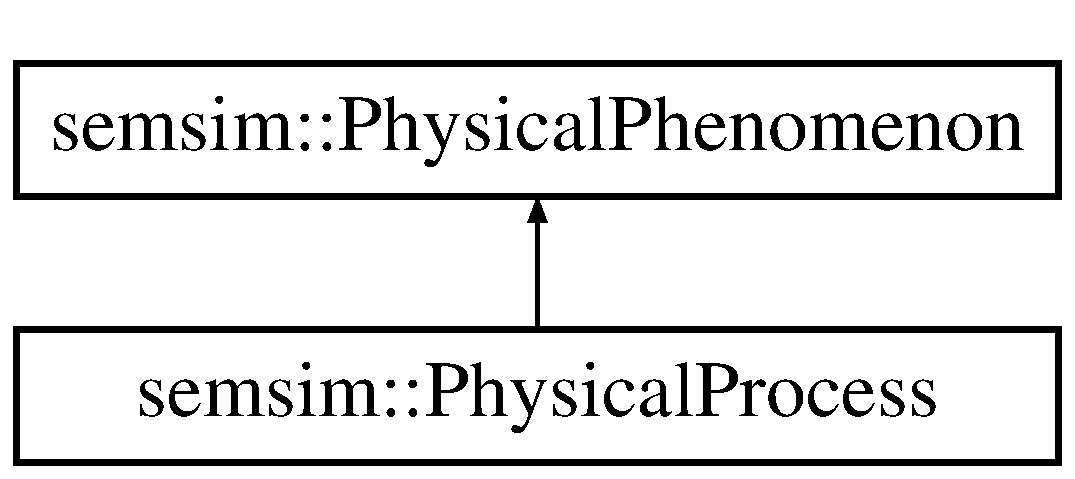
\includegraphics[height=2.000000cm]{classsemsim_1_1PhysicalProcess}
\end{center}
\end{figure}
\subsection*{Public Member Functions}
\begin{DoxyCompactItemize}
\item 
\mbox{\Hypertarget{classsemsim_1_1PhysicalProcess_ae000179654944f3e35b20485d2f0adf0}\label{classsemsim_1_1PhysicalProcess_ae000179654944f3e35b20485d2f0adf0}} 
{\bfseries Physical\+Process} (librdf\+\_\+model $\ast$model, \hyperlink{classsemsim_1_1Subject}{Subject} metaid, \hyperlink{classsemsim_1_1PhysicalPropertyResource}{Physical\+Property\+Resource} physical\+Property, Sources sources, Sinks sinks, Mediators mediators)
\item 
\mbox{\Hypertarget{classsemsim_1_1PhysicalProcess_abe6be94626981d15e27615e040fdda2f}\label{classsemsim_1_1PhysicalProcess_abe6be94626981d15e27615e040fdda2f}} 
void {\bfseries free} () override
\item 
\mbox{\Hypertarget{classsemsim_1_1PhysicalProcess_aaf6d4c0263198fc9355ca4d74221f35d}\label{classsemsim_1_1PhysicalProcess_aaf6d4c0263198fc9355ca4d74221f35d}} 
{\bfseries Physical\+Process} (librdf\+\_\+model $\ast$model)
\item 
\mbox{\Hypertarget{classsemsim_1_1PhysicalProcess_a6d3ea622c0f1fa642068b1b7e76385e5}\label{classsemsim_1_1PhysicalProcess_a6d3ea622c0f1fa642068b1b7e76385e5}} 
const Sources \& {\bfseries get\+Sources} () const
\item 
\mbox{\Hypertarget{classsemsim_1_1PhysicalProcess_aa7ec750398cf738c374c9e92c0bb5670}\label{classsemsim_1_1PhysicalProcess_aa7ec750398cf738c374c9e92c0bb5670}} 
const Sinks \& {\bfseries get\+Sinks} () const
\item 
\mbox{\Hypertarget{classsemsim_1_1PhysicalProcess_a127806bf74ec1e31514c6f3d659824b3}\label{classsemsim_1_1PhysicalProcess_a127806bf74ec1e31514c6f3d659824b3}} 
const Mediators \& {\bfseries get\+Mediators} () const
\item 
\mbox{\Hypertarget{classsemsim_1_1PhysicalProcess_a90d27a6f08b58a7917da00dfbfb5ff72}\label{classsemsim_1_1PhysicalProcess_a90d27a6f08b58a7917da00dfbfb5ff72}} 
\hyperlink{classsemsim_1_1Triples}{Triples} {\bfseries to\+Triples} () override
\item 
\mbox{\Hypertarget{classsemsim_1_1PhysicalProcess_a1caf11364214c1f0e379729e92333208}\label{classsemsim_1_1PhysicalProcess_a1caf11364214c1f0e379729e92333208}} 
\hyperlink{classsemsim_1_1PhysicalProcess}{Physical\+Process} \& {\bfseries set\+About} (std\+::string metaid)
\item 
\mbox{\Hypertarget{classsemsim_1_1PhysicalProcess_a5b0b6e6d5eba493fed10759497057f1b}\label{classsemsim_1_1PhysicalProcess_a5b0b6e6d5eba493fed10759497057f1b}} 
\hyperlink{classsemsim_1_1PhysicalProcess}{Physical\+Process} \& {\bfseries set\+Physical\+Property} (const std\+::string \&physical\+Property)
\item 
\mbox{\Hypertarget{classsemsim_1_1PhysicalProcess_ad5015bd89fef10553e03f0f6b4b13085}\label{classsemsim_1_1PhysicalProcess_ad5015bd89fef10553e03f0f6b4b13085}} 
\hyperlink{classsemsim_1_1PhysicalProcess}{Physical\+Process} \& {\bfseries set\+Physical\+Property} (\hyperlink{classsemsim_1_1PhysicalPropertyResource}{Physical\+Property\+Resource} physical\+Property)
\item 
\mbox{\Hypertarget{classsemsim_1_1PhysicalProcess_a28eeb2d8344664a842b725249bea7dec}\label{classsemsim_1_1PhysicalProcess_a28eeb2d8344664a842b725249bea7dec}} 
\hyperlink{classsemsim_1_1PhysicalProcess}{Physical\+Process} \& {\bfseries add\+Source} (std\+::string source\+\_\+metaid, double multiplier, std\+::string physical\+\_\+entity\+\_\+reference)
\item 
\mbox{\Hypertarget{classsemsim_1_1PhysicalProcess_a88c77abfb77d9a006da62fd0c0730007}\label{classsemsim_1_1PhysicalProcess_a88c77abfb77d9a006da62fd0c0730007}} 
\hyperlink{classsemsim_1_1PhysicalProcess}{Physical\+Process} \& {\bfseries add\+Sink} (std\+::string sink\+\_\+metaid, double multiplier, std\+::string physical\+\_\+entity\+\_\+reference)
\item 
\mbox{\Hypertarget{classsemsim_1_1PhysicalProcess_a798bda68e6b2fb7940e3400b003c1d7d}\label{classsemsim_1_1PhysicalProcess_a798bda68e6b2fb7940e3400b003c1d7d}} 
\hyperlink{classsemsim_1_1PhysicalProcess}{Physical\+Process} \& {\bfseries add\+Mediator} (std\+::string mediator\+\_\+metaid, double multiplier, std\+::string physical\+\_\+entity\+\_\+reference)
\item 
\mbox{\Hypertarget{classsemsim_1_1PhysicalProcess_a07fa014685889073952834086b3a74a4}\label{classsemsim_1_1PhysicalProcess_a07fa014685889073952834086b3a74a4}} 
int {\bfseries get\+Num\+Sources} ()
\item 
\mbox{\Hypertarget{classsemsim_1_1PhysicalProcess_a66d037746715d730964329cccc5e68ba}\label{classsemsim_1_1PhysicalProcess_a66d037746715d730964329cccc5e68ba}} 
int {\bfseries get\+Num\+Sinks} ()
\item 
\mbox{\Hypertarget{classsemsim_1_1PhysicalProcess_a6223cd90d08c19c4c81f4c72ffb1379b}\label{classsemsim_1_1PhysicalProcess_a6223cd90d08c19c4c81f4c72ffb1379b}} 
int {\bfseries get\+Num\+Mediators} ()
\end{DoxyCompactItemize}
\subsection*{Additional Inherited Members}


The documentation for this class was generated from the following files\+:\begin{DoxyCompactItemize}
\item 
src/semsim/Physical\+Process.\+h\item 
src/semsim/Physical\+Process.\+cpp\end{DoxyCompactItemize}

\hypertarget{classsemsim_1_1PhysicalPropertyResource}{}\doxysection{semsim\+::Physical\+Property\+Resource Class Reference}
\label{classsemsim_1_1PhysicalPropertyResource}\index{semsim::PhysicalPropertyResource@{semsim::PhysicalPropertyResource}}
Inheritance diagram for semsim\+::Physical\+Property\+Resource\+:\begin{figure}[H]
                                                                     \begin{center}
                                                                         \leavevmode
                                                                         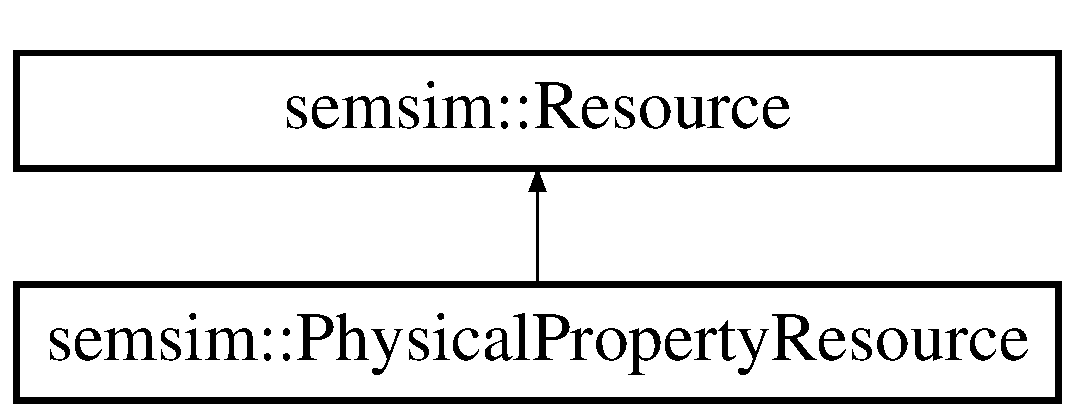
\includegraphics[height=2.000000cm]{classsemsim_1_1PhysicalPropertyResource}
                                                                     \end{center}
\end{figure}
\doxysubsection*{Public Member Functions}
\begin{DoxyCompactItemize}
    \item
    \mbox{\Hypertarget{classsemsim_1_1PhysicalPropertyResource_af693aadda24b00c2c26762079bff6847}\label{classsemsim_1_1PhysicalPropertyResource_af693aadda24b00c2c26762079bff6847}}
    {\bfseries Physical\+Property\+Resource} (Librdf\+World world, \mbox{\hyperlink{classsemsim_1_1RDFURINode}{R\+D\+F\+U\+R\+I\+Node}} node)
    \item
    \mbox{\Hypertarget{classsemsim_1_1PhysicalPropertyResource_a39243d041708d44ed7fee1734c006054}\label{classsemsim_1_1PhysicalPropertyResource_a39243d041708d44ed7fee1734c006054}}
    {\bfseries Physical\+Property\+Resource} (Librdf\+World world, std\+::string node)
    \item
    \mbox{\Hypertarget{classsemsim_1_1PhysicalPropertyResource_a2368cabb4268b7869dc550caca498d36}\label{classsemsim_1_1PhysicalPropertyResource_a2368cabb4268b7869dc550caca498d36}}
    \mbox{\hyperlink{classsemsim_1_1Triple}{Triple}} {\bfseries is\+Version\+Of\+Triple} (std\+::string subject\+\_\+metaid) const
    \item
    \mbox{\Hypertarget{classsemsim_1_1PhysicalPropertyResource_a9b8353de4178fc6d10ef64fdf8a0d0f7}\label{classsemsim_1_1PhysicalPropertyResource_a9b8353de4178fc6d10ef64fdf8a0d0f7}}
    \mbox{\hyperlink{classsemsim_1_1Triple}{Triple}} {\bfseries is\+Property\+Of\+Triple} (std\+::string subject\+\_\+metaid, std\+::string property\+\_\+metaid) const
    \item
    \mbox{\Hypertarget{classsemsim_1_1PhysicalPropertyResource_a39c3c740dfcddcfc57c32e46894db4cc}\label{classsemsim_1_1PhysicalPropertyResource_a39c3c740dfcddcfc57c32e46894db4cc}}
    \mbox{\hyperlink{classsemsim_1_1Triples}{Triples}} {\bfseries to\+Triples} (std\+::string subject\+\_\+metaid, std\+::string property\+\_\+metaid) const
    \item
    \mbox{\Hypertarget{classsemsim_1_1PhysicalPropertyResource_afea7c0c29e019e7f3756d8a646c9a8b6}\label{classsemsim_1_1PhysicalPropertyResource_afea7c0c29e019e7f3756d8a646c9a8b6}}
    bool {\bfseries is\+Set} () const override
\end{DoxyCompactItemize}
\doxysubsection*{Additional Inherited Members}


The documentation for this class was generated from the following files\+:\begin{DoxyCompactItemize}
                                                                              \item
                                                                              src/semsim/Physical\+Property\+Resource.\+h\item
                                                                              src/semsim/Physical\+Property\+Resource.\+cpp
\end{DoxyCompactItemize}

\hypertarget{classsemsim_1_1Predicate}{}\section{semsim\+:\+:Predicate Class Reference}
\label{classsemsim_1_1Predicate}\index{semsim\+::\+Predicate@{semsim\+::\+Predicate}}
Inheritance diagram for semsim\+:\+:Predicate\+:\begin{figure}[H]
\begin{center}
\leavevmode
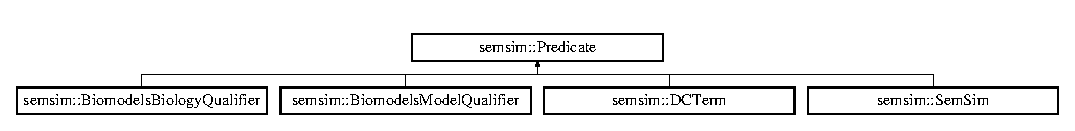
\includegraphics[height=1.308411cm]{classsemsim_1_1Predicate}
\end{center}
\end{figure}
\subsection*{Public Member Functions}
\begin{DoxyCompactItemize}
\item 
\mbox{\Hypertarget{classsemsim_1_1Predicate_a111a30f2cf259153b4f186b308b6716f}\label{classsemsim_1_1Predicate_a111a30f2cf259153b4f186b308b6716f}} 
{\bfseries Predicate} (const std\+::string \&namespace\+\_\+, std\+::string term, std\+::string prefix)
\item 
\mbox{\Hypertarget{classsemsim_1_1Predicate_a47fed0b10781d69cc6e359bcec16eb71}\label{classsemsim_1_1Predicate_a47fed0b10781d69cc6e359bcec16eb71}} 
std\+::string {\bfseries str} ()
\item 
\mbox{\Hypertarget{classsemsim_1_1Predicate_a6e4ea55d33e692cdb894940c3708cabb}\label{classsemsim_1_1Predicate_a6e4ea55d33e692cdb894940c3708cabb}} 
librdf\+\_\+node $\ast$ {\bfseries get\+Node} () const
\item 
\mbox{\Hypertarget{classsemsim_1_1Predicate_a4a1ffe837216303654416b725684b9db}\label{classsemsim_1_1Predicate_a4a1ffe837216303654416b725684b9db}} 
const std\+::vector$<$ std\+::string $>$ \& {\bfseries get\+Valid\+Terms} () const
\item 
\mbox{\Hypertarget{classsemsim_1_1Predicate_aefb90236a7934d93cce5798723f54661}\label{classsemsim_1_1Predicate_aefb90236a7934d93cce5798723f54661}} 
const std\+::string \& {\bfseries get\+Namespace} () const
\item 
\mbox{\Hypertarget{classsemsim_1_1Predicate_a1a62bbbe1ac5e3a28a15fda049d4ada4}\label{classsemsim_1_1Predicate_a1a62bbbe1ac5e3a28a15fda049d4ada4}} 
const std\+::string \& {\bfseries get\+Term} () const
\item 
\mbox{\Hypertarget{classsemsim_1_1Predicate_ad7115549cf9b25cbb665f5c2bcba67d4}\label{classsemsim_1_1Predicate_ad7115549cf9b25cbb665f5c2bcba67d4}} 
const std\+::string \& {\bfseries get\+Prefix} () const
\item 
\mbox{\Hypertarget{classsemsim_1_1Predicate_add37b6df8a8bf63600966a3ab24236d9}\label{classsemsim_1_1Predicate_add37b6df8a8bf63600966a3ab24236d9}} 
const std\+::string \& {\bfseries get\+Uri} () const
\item 
\mbox{\Hypertarget{classsemsim_1_1Predicate_aa8a95f5f9e0bffbb8d6df9c8767a6b01}\label{classsemsim_1_1Predicate_aa8a95f5f9e0bffbb8d6df9c8767a6b01}} 
void {\bfseries free\+Node} ()
\item 
\mbox{\Hypertarget{classsemsim_1_1Predicate_a56b15a4d95c7f6e4645e954e5d5d3d13}\label{classsemsim_1_1Predicate_a56b15a4d95c7f6e4645e954e5d5d3d13}} 
void {\bfseries set\+Node} (librdf\+\_\+node $\ast$node)
\end{DoxyCompactItemize}
\subsection*{Static Public Member Functions}
\begin{DoxyCompactItemize}
\item 
\mbox{\Hypertarget{classsemsim_1_1Predicate_a332f745e39155ff5884e2c98c87b548b}\label{classsemsim_1_1Predicate_a332f745e39155ff5884e2c98c87b548b}} 
static std\+::unordered\+\_\+map$<$ std\+::string, std\+::string $>$ {\bfseries namespace\+Map} ()
\item 
\mbox{\Hypertarget{classsemsim_1_1Predicate_a3e4b6a9dd8180026ef09d8234076655f}\label{classsemsim_1_1Predicate_a3e4b6a9dd8180026ef09d8234076655f}} 
static void {\bfseries verify} (std\+::vector$<$ std\+::string $>$ valid\+\_\+terms, const std\+::string \&term)
\item 
\mbox{\Hypertarget{classsemsim_1_1Predicate_a514f441587bc049f53666c55a5d645ce}\label{classsemsim_1_1Predicate_a514f441587bc049f53666c55a5d645ce}} 
static bool {\bfseries namespace\+Known} (const std\+::string \&ns)
\item 
\mbox{\Hypertarget{classsemsim_1_1Predicate_a47b3b6a018b2d1085c0feaf504e12568}\label{classsemsim_1_1Predicate_a47b3b6a018b2d1085c0feaf504e12568}} 
static void {\bfseries add\+Seen\+Namespace\+To\+Serializer} (librdf\+\_\+world $\ast$world, librdf\+\_\+serializer $\ast$serializer, librdf\+\_\+node $\ast$predicate)
\end{DoxyCompactItemize}
\subsection*{Protected Member Functions}
\begin{DoxyCompactItemize}
\item 
\mbox{\Hypertarget{classsemsim_1_1Predicate_a90af4d016315412f8fd64d9ec280b177}\label{classsemsim_1_1Predicate_a90af4d016315412f8fd64d9ec280b177}} 
{\bfseries Predicate} (librdf\+\_\+node $\ast$node)
\end{DoxyCompactItemize}
\subsection*{Protected Attributes}
\begin{DoxyCompactItemize}
\item 
\mbox{\Hypertarget{classsemsim_1_1Predicate_ad74a27f704532cdc6a80e094c2d5b3f4}\label{classsemsim_1_1Predicate_ad74a27f704532cdc6a80e094c2d5b3f4}} 
std\+::string {\bfseries namespace\+\_\+}
\item 
\mbox{\Hypertarget{classsemsim_1_1Predicate_acb9c36ea2356d2b8791a2e8ad9cf68eb}\label{classsemsim_1_1Predicate_acb9c36ea2356d2b8791a2e8ad9cf68eb}} 
std\+::string {\bfseries term\+\_\+}
\item 
\mbox{\Hypertarget{classsemsim_1_1Predicate_acb69247cf1ff304bfaec2df1755b4654}\label{classsemsim_1_1Predicate_acb69247cf1ff304bfaec2df1755b4654}} 
std\+::string {\bfseries prefix\+\_\+}
\item 
\mbox{\Hypertarget{classsemsim_1_1Predicate_a6ceaeb4b2a9a431cfdfe537be842edd2}\label{classsemsim_1_1Predicate_a6ceaeb4b2a9a431cfdfe537be842edd2}} 
std\+::string {\bfseries uri\+\_\+}
\item 
\mbox{\Hypertarget{classsemsim_1_1Predicate_a9a488e0bf03949975fa54d2de0b2fd58}\label{classsemsim_1_1Predicate_a9a488e0bf03949975fa54d2de0b2fd58}} 
librdf\+\_\+node $\ast$ {\bfseries node\+\_\+} = nullptr
\item 
\mbox{\Hypertarget{classsemsim_1_1Predicate_aaffa9838c17b7bc7c33559ef1253a594}\label{classsemsim_1_1Predicate_aaffa9838c17b7bc7c33559ef1253a594}} 
std\+::vector$<$ std\+::string $>$ \hyperlink{classsemsim_1_1Predicate_aaffa9838c17b7bc7c33559ef1253a594}{valid\+\_\+terms\+\_\+} \{\char`\"{}All\char`\"{}\}
\begin{DoxyCompactList}\small\item\em predicates can only have type uri \end{DoxyCompactList}\end{DoxyCompactItemize}


The documentation for this class was generated from the following files\+:\begin{DoxyCompactItemize}
\item 
src/semsim/Predicate.\+h\item 
src/semsim/Predicate.\+cpp\end{DoxyCompactItemize}

\hypertarget{classsemsim_1_1Query}{}\section{semsim\+:\+:Query Class Reference}
\label{classsemsim_1_1Query}\index{semsim\+::\+Query@{semsim\+::\+Query}}
\subsection*{\+: variable name}
\label{_amgrp7ca1d8b10bb02d408ac42bd6ecaaf12b}%
librdf\+\_\+query\+\_\+results\+\_\+get\+\_\+binding\+\_\+value\+\_\+by\+\_\+name\+: \+: \#librdf\+\_\+query\+\_\+results query results

Get one binding value for a given name in the current result.

Return value\+: a new \#librdf\+\_\+node binding value or N\+U\+LL on failure \begin{DoxyCompactItemize}
\item 
\mbox{\Hypertarget{classsemsim_1_1Query_adc98ca404ecad9f4fd4f718c92721211}\label{classsemsim_1_1Query_adc98ca404ecad9f4fd4f718c92721211}} 
{\bfseries Query} (librdf\+\_\+model $\ast$model, std\+::string query)
\item 
\mbox{\Hypertarget{classsemsim_1_1Query_a16a28232cd8bf950b1e76e017ec93561}\label{classsemsim_1_1Query_a16a28232cd8bf950b1e76e017ec93561}} 
{\bfseries Query} (const \hyperlink{classsemsim_1_1Query}{Query} \&query)=delete
\item 
\mbox{\Hypertarget{classsemsim_1_1Query_a1edd5ec1cd5cb057121fa0b35fad48ec}\label{classsemsim_1_1Query_a1edd5ec1cd5cb057121fa0b35fad48ec}} 
{\bfseries Query} (\hyperlink{classsemsim_1_1Query}{Query} \&\&query) noexcept
\item 
\mbox{\Hypertarget{classsemsim_1_1Query_ae76fa75112392cfdc176c7a7ee6912f2}\label{classsemsim_1_1Query_ae76fa75112392cfdc176c7a7ee6912f2}} 
\hyperlink{classsemsim_1_1Query}{Query} \& {\bfseries operator=} (const \hyperlink{classsemsim_1_1Query}{Query} \&query)=delete
\item 
\mbox{\Hypertarget{classsemsim_1_1Query_a3b7646a5d2722ff4d1962c3f0a620882}\label{classsemsim_1_1Query_a3b7646a5d2722ff4d1962c3f0a620882}} 
\hyperlink{classsemsim_1_1Query}{Query} \& {\bfseries operator=} (\hyperlink{classsemsim_1_1Query}{Query} \&\&query) noexcept
\item 
\mbox{\Hypertarget{classsemsim_1_1Query_a8b74d77f2c4fbcd9800548aa4c4304ec}\label{classsemsim_1_1Query_a8b74d77f2c4fbcd9800548aa4c4304ec}} 
void {\bfseries free\+Query} ()
\item 
\mbox{\Hypertarget{classsemsim_1_1Query_a83580c1b66d2d052696dd907e8594a8a}\label{classsemsim_1_1Query_a83580c1b66d2d052696dd907e8594a8a}} 
librdf\+\_\+stream $\ast$ {\bfseries results\+As\+Lib\+Rdf\+Stream} ()
\item 
\mbox{\Hypertarget{classsemsim_1_1Query_a16b43e8d44b25e0d1fba34c73c5386dc}\label{classsemsim_1_1Query_a16b43e8d44b25e0d1fba34c73c5386dc}} 
Results\+Map {\bfseries results\+As\+Map} ()
\item 
\mbox{\Hypertarget{classsemsim_1_1Query_ae44b7aff3ae00151f63cc3a355705091}\label{classsemsim_1_1Query_ae44b7aff3ae00151f63cc3a355705091}} 
std\+::string {\bfseries results\+As\+Str} (const std\+::string \&output\+\_\+format)
\item 
\mbox{\Hypertarget{classsemsim_1_1Query_ad629d8d9265fdc07dc88a698de69f2d9}\label{classsemsim_1_1Query_ad629d8d9265fdc07dc88a698de69f2d9}} 
void {\bfseries run\+Query} ()
\end{DoxyCompactItemize}


The documentation for this class was generated from the following files\+:\begin{DoxyCompactItemize}
\item 
src/semsim/Query.\+h\item 
src/semsim/Query.\+cpp\end{DoxyCompactItemize}

\hypertarget{classredland_1_1RaptorIOStream}{}\section{redland\+:\+:Raptor\+I\+O\+Stream Class Reference}
\label{classredland_1_1RaptorIOStream}\index{redland\+::\+Raptor\+I\+O\+Stream@{redland\+::\+Raptor\+I\+O\+Stream}}
\subsection*{Public Member Functions}
\begin{DoxyCompactItemize}
\item 
\mbox{\Hypertarget{classredland_1_1RaptorIOStream_a6cf2e1a9cf6c31bb37069c5b3e591509}\label{classredland_1_1RaptorIOStream_a6cf2e1a9cf6c31bb37069c5b3e591509}} 
{\bfseries Raptor\+I\+O\+Stream} (raptor\+\_\+iostream $\ast$iostream)
\item 
\mbox{\Hypertarget{classredland_1_1RaptorIOStream_adbcfcc29e030219dfd180ecb3d6c2c4b}\label{classredland_1_1RaptorIOStream_adbcfcc29e030219dfd180ecb3d6c2c4b}} 
raptor\+\_\+iostream $\ast$ {\bfseries get} () const
\end{DoxyCompactItemize}
\subsection*{Static Public Member Functions}
\begin{DoxyCompactItemize}
\item 
\mbox{\Hypertarget{classredland_1_1RaptorIOStream_ab4b78aede5b54be5a654c9b81e65452c}\label{classredland_1_1RaptorIOStream_ab4b78aede5b54be5a654c9b81e65452c}} 
static std\+::pair$<$ \hyperlink{classredland_1_1RaptorIOStream}{Raptor\+I\+O\+Stream}, void $\ast$ $>$ {\bfseries new\+I\+O\+To\+String} ()
\end{DoxyCompactItemize}


The documentation for this class was generated from the following files\+:\begin{DoxyCompactItemize}
\item 
src/redland/\+Redland\+A\+P\+I\+Wrapper/src/Raptor\+I\+O\+Stream.\+h\item 
src/redland/\+Redland\+A\+P\+I\+Wrapper/src/Raptor\+I\+O\+Stream.\+cpp\end{DoxyCompactItemize}

\hypertarget{classsemsim_1_1RDF}{}\section{semsim\+:\+:R\+DF Class Reference}
\label{classsemsim_1_1RDF}\index{semsim\+::\+R\+DF@{semsim\+::\+R\+DF}}
\subsection*{Public Member Functions}
\begin{DoxyCompactItemize}
\item 
\mbox{\Hypertarget{classsemsim_1_1RDF_adb3d644393c659dc3cd54b29d6bfaec0}\label{classsemsim_1_1RDF_adb3d644393c659dc3cd54b29d6bfaec0}} 
{\bfseries R\+DF} (const std\+::string \&base\+\_\+uri=\char`\"{}./Annotations.\+rdf\char`\"{}, const std\+::string \&storage\+\_\+type=\char`\"{}memory\char`\"{}, const std\+::string \&storage\+\_\+name=\char`\"{}Semsim\+Store\char`\"{}, const char $\ast$storage\+\_\+options=nullptr, const char $\ast$model\+\_\+options=nullptr)
\item 
\mbox{\Hypertarget{classsemsim_1_1RDF_aefd8c1ee16d47a49ce3e2828b7671866}\label{classsemsim_1_1RDF_aefd8c1ee16d47a49ce3e2828b7671866}} 
void {\bfseries free\+R\+DF} ()
\item 
\mbox{\Hypertarget{classsemsim_1_1RDF_a1d640ed0ead4d4699c59641a32f6a81a}\label{classsemsim_1_1RDF_a1d640ed0ead4d4699c59641a32f6a81a}} 
{\bfseries R\+DF} (const \hyperlink{classsemsim_1_1RDF}{R\+DF} \&rdf)=delete
\item 
\mbox{\Hypertarget{classsemsim_1_1RDF_ad6e8d742af0aff97c89746a8eaf50777}\label{classsemsim_1_1RDF_ad6e8d742af0aff97c89746a8eaf50777}} 
{\bfseries R\+DF} (\hyperlink{classsemsim_1_1RDF}{R\+DF} \&\&rdf) noexcept
\item 
\mbox{\Hypertarget{classsemsim_1_1RDF_a6a8c2040f0fb2be58380d09ff396f11e}\label{classsemsim_1_1RDF_a6a8c2040f0fb2be58380d09ff396f11e}} 
\hyperlink{classsemsim_1_1RDF}{R\+DF} \& {\bfseries operator=} (const \hyperlink{classsemsim_1_1RDF}{R\+DF} \&rdf)=delete
\item 
\mbox{\Hypertarget{classsemsim_1_1RDF_a0195811b138d141d7944ed475b098189}\label{classsemsim_1_1RDF_a0195811b138d141d7944ed475b098189}} 
\hyperlink{classsemsim_1_1RDF}{R\+DF} \& {\bfseries operator=} (\hyperlink{classsemsim_1_1RDF}{R\+DF} \&\&rdf) noexcept
\item 
\mbox{\Hypertarget{classsemsim_1_1RDF_aec42881cdaeeaffdc91238f03a1db2e6}\label{classsemsim_1_1RDF_aec42881cdaeeaffdc91238f03a1db2e6}} 
int {\bfseries size} () const
\item 
\mbox{\Hypertarget{classsemsim_1_1RDF_a6bbd8747ca3893339162bbb00e9f428f}\label{classsemsim_1_1RDF_a6bbd8747ca3893339162bbb00e9f428f}} 
void {\bfseries set\+Base\+Uri} (std\+::string base\+Uri)
\item 
\mbox{\Hypertarget{classsemsim_1_1RDF_ac90c8d0c73127e851825e1426ce9622e}\label{classsemsim_1_1RDF_ac90c8d0c73127e851825e1426ce9622e}} 
bool {\bfseries empty} () const
\item 
\mbox{\Hypertarget{classsemsim_1_1RDF_a3a920ea30103f06343d4714987a2b765}\label{classsemsim_1_1RDF_a3a920ea30103f06343d4714987a2b765}} 
void {\bfseries add\+From\+String} (const std\+::string \&str, const std\+::string \&format=\char`\"{}guess\char`\"{}, const std\+::string \&base\+\_\+uri=std\+::string())
\item 
\mbox{\Hypertarget{classsemsim_1_1RDF_a27497273858cca1463a612f92f332da1}\label{classsemsim_1_1RDF_a27497273858cca1463a612f92f332da1}} 
void {\bfseries add\+From\+Uri} (const std\+::string \&uri\+\_\+string, const std\+::string \&format=\char`\"{}guess\char`\"{})
\item 
\mbox{\Hypertarget{classsemsim_1_1RDF_a8cd65868da05f409c37b91acdbf33aa0}\label{classsemsim_1_1RDF_a8cd65868da05f409c37b91acdbf33aa0}} 
void {\bfseries add\+From\+File} (const std\+::string \&filename, const std\+::string \&format)
\item 
\mbox{\Hypertarget{classsemsim_1_1RDF_a493ffd6ebc12adc6c668f04f21ce2380}\label{classsemsim_1_1RDF_a493ffd6ebc12adc6c668f04f21ce2380}} 
std\+::unordered\+\_\+map$<$ std\+::string, std\+::string $>$ {\bfseries propagate\+Namespaces\+From\+Parser} (const std\+::vector$<$ std\+::string $>$ \&seen\+\_\+namespaces)
\item 
\mbox{\Hypertarget{classsemsim_1_1RDF_a762cc1d30484cd95b130526e2fab9ef3}\label{classsemsim_1_1RDF_a762cc1d30484cd95b130526e2fab9ef3}} 
std\+::string {\bfseries to\+String} (const std\+::string \&format=\char`\"{}rdfxml-\/abbrev\char`\"{}, std\+::string base\+\_\+uri=std\+::string(), const char $\ast$mime\+\_\+type=nullptr, const char $\ast$type\+\_\+uri=nullptr)
\item 
\mbox{\Hypertarget{classsemsim_1_1RDF_acf46cf3b2dbfa5828dac1e823cf972c8}\label{classsemsim_1_1RDF_acf46cf3b2dbfa5828dac1e823cf972c8}} 
\hyperlink{classsemsim_1_1Editor}{Editor} {\bfseries to\+Editor} (const std\+::string \&xml, Semsim\+Xml\+Type type)
\item 
\mbox{\Hypertarget{classsemsim_1_1RDF_a1f6a4f82d01c93be36eb5c986c1629bc}\label{classsemsim_1_1RDF_a1f6a4f82d01c93be36eb5c986c1629bc}} 
\hyperlink{classsemsim_1_1Editor}{Editor} $\ast$ {\bfseries to\+Editor\+Ptr} (const std\+::string \&xml, Semsim\+Xml\+Type type)
\item 
\mbox{\Hypertarget{classsemsim_1_1RDF_ac8286394b938d0511e7ccbf81583277c}\label{classsemsim_1_1RDF_ac8286394b938d0511e7ccbf81583277c}} 
librdf\+\_\+model $\ast$ {\bfseries get\+Model} () const
\item 
\mbox{\Hypertarget{classsemsim_1_1RDF_a92ace04b947ccd8c7c3c90a4d9d77edb}\label{classsemsim_1_1RDF_a92ace04b947ccd8c7c3c90a4d9d77edb}} 
librdf\+\_\+storage $\ast$ {\bfseries get\+Storage} () const
\end{DoxyCompactItemize}
\subsection*{Static Public Member Functions}
\begin{DoxyCompactItemize}
\item 
\mbox{\Hypertarget{classsemsim_1_1RDF_a77782a3756ed6243ee9b842c6b0f06b8}\label{classsemsim_1_1RDF_a77782a3756ed6243ee9b842c6b0f06b8}} 
static \hyperlink{classsemsim_1_1RDF}{R\+DF} {\bfseries from\+String} (const std\+::string \&str, const std\+::string \&format=\char`\"{}guess\char`\"{}, const std\+::string \&base\+\_\+uri=std\+::string())
\item 
\mbox{\Hypertarget{classsemsim_1_1RDF_a3d14028f5953a4e007cfe8f9a34b3e0d}\label{classsemsim_1_1RDF_a3d14028f5953a4e007cfe8f9a34b3e0d}} 
static \hyperlink{classsemsim_1_1RDF}{R\+DF} {\bfseries from\+Uri} (const std\+::string \&uri\+\_\+string, const std\+::string \&format=\char`\"{}guess\char`\"{})
\item 
\mbox{\Hypertarget{classsemsim_1_1RDF_ab5f969412a37a4ecad5f8485177ae561}\label{classsemsim_1_1RDF_ab5f969412a37a4ecad5f8485177ae561}} 
static \hyperlink{classsemsim_1_1RDF}{R\+DF} {\bfseries from\+File} (const std\+::string \&filename, const std\+::string \&format)
\item 
\mbox{\Hypertarget{classsemsim_1_1RDF_ab1c83f13027f0946d08dd21368706f3b}\label{classsemsim_1_1RDF_ab1c83f13027f0946d08dd21368706f3b}} 
static void {\bfseries from\+String} (\hyperlink{classsemsim_1_1RDF}{R\+DF} $\ast$rdf, const std\+::string \&str, const std\+::string \&format, const std\+::string \&base\+\_\+uri)
\end{DoxyCompactItemize}
\subsection*{Public Attributes}
\begin{DoxyCompactItemize}
\item 
\mbox{\Hypertarget{classsemsim_1_1RDF_a03a6df29bae51bba853a11d5eb433835}\label{classsemsim_1_1RDF_a03a6df29bae51bba853a11d5eb433835}} 
std\+::string {\bfseries base\+\_\+uri\+\_\+}
\item 
\mbox{\Hypertarget{classsemsim_1_1RDF_a106ee70106beb1c1304c8968470f3033}\label{classsemsim_1_1RDF_a106ee70106beb1c1304c8968470f3033}} 
Namespace\+Map {\bfseries namespaces\+\_\+}
\item 
\mbox{\Hypertarget{classsemsim_1_1RDF_af3bbb4dc4ce350bf60fc6a94bffd41b2}\label{classsemsim_1_1RDF_af3bbb4dc4ce350bf60fc6a94bffd41b2}} 
std\+::vector$<$ std\+::string $>$ {\bfseries seen\+\_\+namespaces\+\_\+}
\item 
Namespace\+Map {\bfseries default\+\_\+namespaces\+\_\+}
\end{DoxyCompactItemize}


\subsection{Member Data Documentation}
\mbox{\Hypertarget{classsemsim_1_1RDF_a9a2f19c41f10c772cb4dece71c473bd2}\label{classsemsim_1_1RDF_a9a2f19c41f10c772cb4dece71c473bd2}} 
\index{semsim\+::\+R\+DF@{semsim\+::\+R\+DF}!default\+\_\+namespaces\+\_\+@{default\+\_\+namespaces\+\_\+}}
\index{default\+\_\+namespaces\+\_\+@{default\+\_\+namespaces\+\_\+}!semsim\+::\+R\+DF@{semsim\+::\+R\+DF}}
\subsubsection{\texorpdfstring{default\+\_\+namespaces\+\_\+}{default\_namespaces\_}}
{\footnotesize\ttfamily Namespace\+Map semsim\+::\+R\+D\+F\+::default\+\_\+namespaces\+\_\+}

{\bfseries Initial value\+:}
\begin{DoxyCode}
= \{
                \{\textcolor{stringliteral}{"http://purl.org/dc/terms/"},                \textcolor{stringliteral}{"dcterms"}\},
                \{\textcolor{stringliteral}{"http://biomodels.net/biology-qualifiers/"}, \textcolor{stringliteral}{"bqbiol"}\},
                \{\textcolor{stringliteral}{"http://biomodels.net/model-qualifiers/"},   \textcolor{stringliteral}{"bqmodel"}\},
                \{\textcolor{stringliteral}{"http://www.bhi.washington.edu/semsim#"},    \textcolor{stringliteral}{"semsim"}\},
        \}
\end{DoxyCode}


The documentation for this class was generated from the following files\+:\begin{DoxyCompactItemize}
\item 
src/semsim/R\+D\+F.\+h\item 
src/semsim/R\+D\+F.\+cpp\end{DoxyCompactItemize}

\hypertarget{classRedlandLibrdfException}{}\section{Redland\+Librdf\+Exception Class Reference}
\label{classRedlandLibrdfException}\index{Redland\+Librdf\+Exception@{Redland\+Librdf\+Exception}}
Inheritance diagram for Redland\+Librdf\+Exception\+:\begin{figure}[H]
\begin{center}
\leavevmode
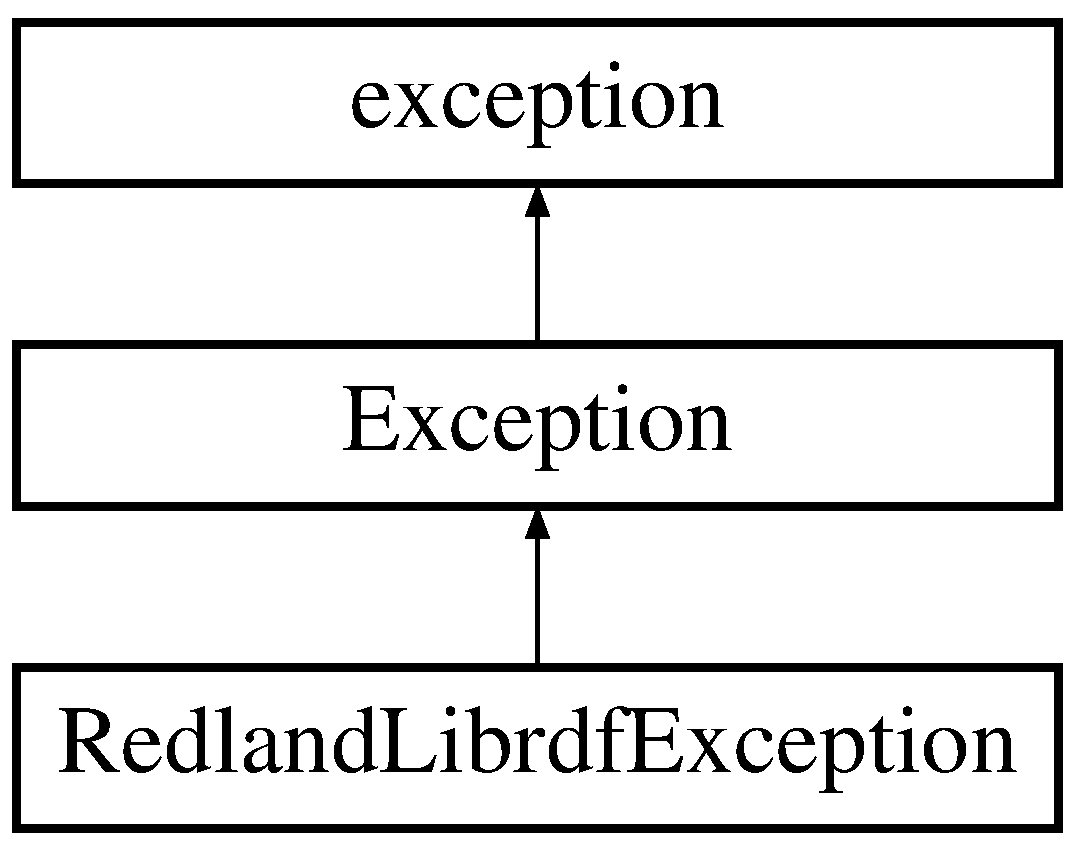
\includegraphics[height=3.000000cm]{classRedlandLibrdfException}
\end{center}
\end{figure}
\subsection*{Additional Inherited Members}


The documentation for this class was generated from the following file\+:\begin{DoxyCompactItemize}
\item 
src/redland/\+Redland\+A\+P\+I\+Wrapper/src/Librdf\+Exception.\+h\end{DoxyCompactItemize}

\hypertarget{classRedlandNullPointerException}{}\section{Redland\+Null\+Pointer\+Exception Class Reference}
\label{classRedlandNullPointerException}\index{Redland\+Null\+Pointer\+Exception@{Redland\+Null\+Pointer\+Exception}}
Inheritance diagram for Redland\+Null\+Pointer\+Exception\+:\begin{figure}[H]
\begin{center}
\leavevmode
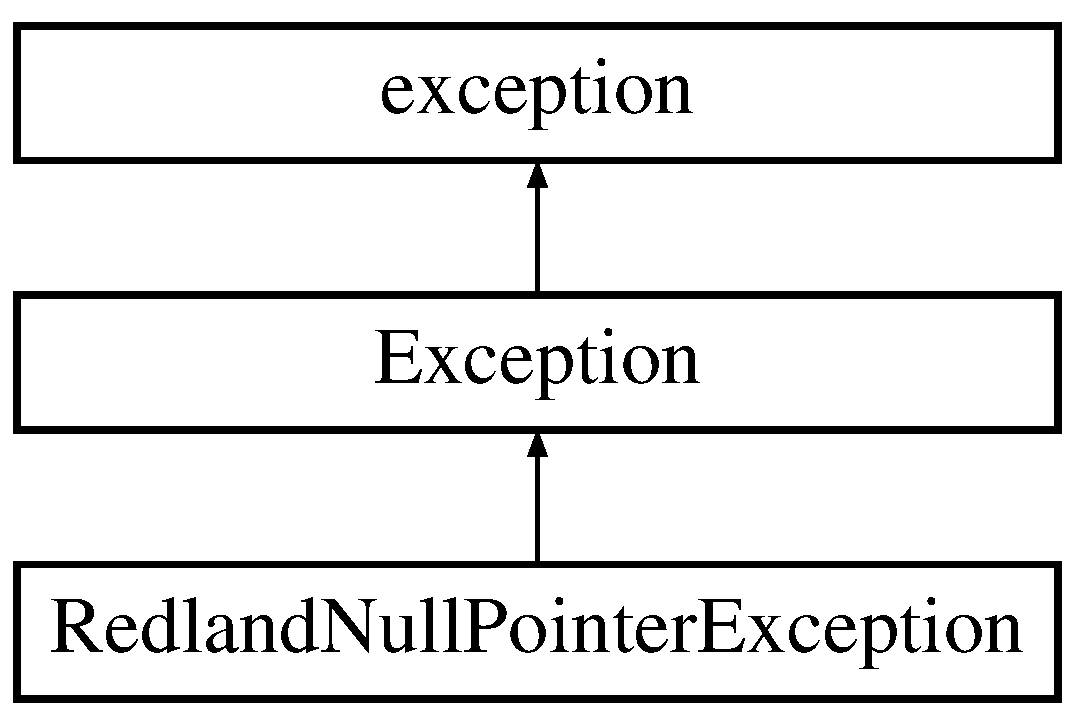
\includegraphics[height=3.000000cm]{classRedlandNullPointerException}
\end{center}
\end{figure}
\subsection*{Additional Inherited Members}


The documentation for this class was generated from the following file\+:\begin{DoxyCompactItemize}
\item 
src/redland/\+Redland\+A\+P\+I\+Wrapper/src/Librdf\+Exception.\+h\end{DoxyCompactItemize}

\hypertarget{classsemsim_1_1Resource}{}\doxysection{semsim\+::Resource Class Reference}
\label{classsemsim_1_1Resource}\index{semsim::Resource@{semsim::Resource}}
Inheritance diagram for semsim\+::Resource\+:\begin{figure}[H]
                                                 \begin{center}
                                                     \leavevmode
                                                     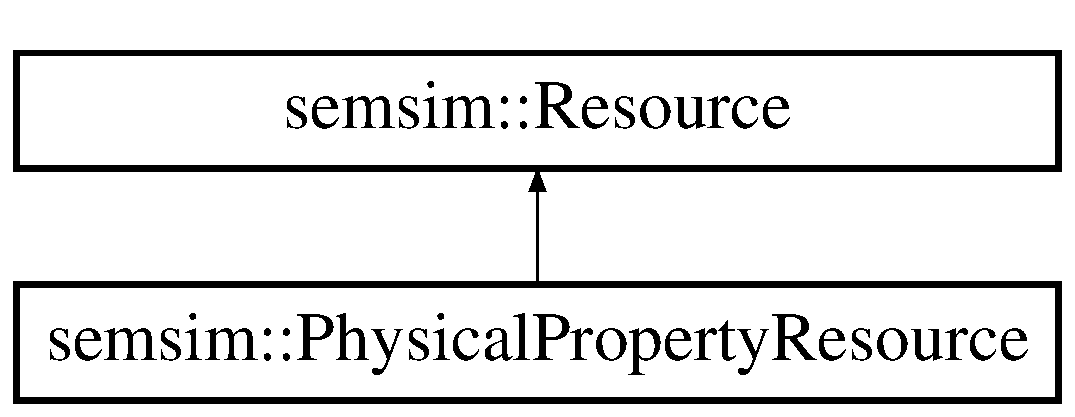
\includegraphics[height=2.000000cm]{classsemsim_1_1Resource}
                                                 \end{center}
\end{figure}
\doxysubsection*{Public Member Functions}
\begin{DoxyCompactItemize}
    \item
    \mbox{\Hypertarget{classsemsim_1_1Resource_ace808d48dfa415cef76a96049971a7d6}\label{classsemsim_1_1Resource_ace808d48dfa415cef76a96049971a7d6}}
    {\bfseries Resource} (Librdf\+World world, const \mbox{\hyperlink{classsemsim_1_1RDFLiteralNode}{R\+D\+F\+Literal\+Node}} \&node)
    \item
    \mbox{\Hypertarget{classsemsim_1_1Resource_a54c5fb0cba8d55bacfea12f16fcd9d15}\label{classsemsim_1_1Resource_a54c5fb0cba8d55bacfea12f16fcd9d15}}
    {\bfseries Resource} (Librdf\+World world, const \mbox{\hyperlink{classsemsim_1_1RDFURINode}{R\+D\+F\+U\+R\+I\+Node}} \&node)
    \item
    \mbox{\Hypertarget{classsemsim_1_1Resource_a0fafe859115b08313ff18b1eb3be521b}\label{classsemsim_1_1Resource_a0fafe859115b08313ff18b1eb3be521b}}
    {\bfseries Resource} (Librdf\+World world, const \mbox{\hyperlink{classsemsim_1_1RDFBlankNode}{R\+D\+F\+Blank\+Node}} \&node)
    \item
    \mbox{\Hypertarget{classsemsim_1_1Resource_abb0bdbdd70a34a3e8ef6ebe2b19b4ad3}\label{classsemsim_1_1Resource_abb0bdbdd70a34a3e8ef6ebe2b19b4ad3}}
    {\bfseries Resource} (Librdf\+World world, Librdf\+Node node)
    \item
    \mbox{\Hypertarget{classsemsim_1_1Resource_ab2a1eb4faf15270e7c6e6d165d751851}\label{classsemsim_1_1Resource_ab2a1eb4faf15270e7c6e6d165d751851}}
    Librdf\+Node {\bfseries get\+Node} () const
    \item
    \mbox{\Hypertarget{classsemsim_1_1Resource_ac762aa68f78bb750d71f4b109395dcfd}\label{classsemsim_1_1Resource_ac762aa68f78bb750d71f4b109395dcfd}}
    std\+::string {\bfseries str} () const
    \item
    \mbox{\Hypertarget{classsemsim_1_1Resource_a46e7e3a2b53852994f689685bb3df555}\label{classsemsim_1_1Resource_a46e7e3a2b53852994f689685bb3df555}}
    virtual bool {\bfseries is\+Set} () const
\end{DoxyCompactItemize}
\doxysubsection*{Protected Attributes}
\begin{DoxyCompactItemize}
    \item
    \mbox{\Hypertarget{classsemsim_1_1Resource_a3f51d0f7fada7133f2d4be0ec6879eff}\label{classsemsim_1_1Resource_a3f51d0f7fada7133f2d4be0ec6879eff}}
    Librdf\+World {\bfseries world\+\_\+}
    \item
    \mbox{\Hypertarget{classsemsim_1_1Resource_ac8a9754709900d4c64f79d20a38f2d1b}\label{classsemsim_1_1Resource_ac8a9754709900d4c64f79d20a38f2d1b}}
    R\+D\+F\+Node\+Ptr {\bfseries rdf\+\_\+node\+\_\+ptr\+\_\+}
\end{DoxyCompactItemize}


The documentation for this class was generated from the following files\+:\begin{DoxyCompactItemize}
                                                                              \item
                                                                              src/semsim/Resource.\+h\item
                                                                              src/semsim/Resource.\+cpp
\end{DoxyCompactItemize}

\hypertarget{classsemsim_1_1SBMLAssistant}{}\section{semsim\+:\+:S\+B\+M\+L\+Assistant Class Reference}
\label{classsemsim_1_1SBMLAssistant}\index{semsim\+::\+S\+B\+M\+L\+Assistant@{semsim\+::\+S\+B\+M\+L\+Assistant}}
Inheritance diagram for semsim\+:\+:S\+B\+M\+L\+Assistant\+:\begin{figure}[H]
\begin{center}
\leavevmode
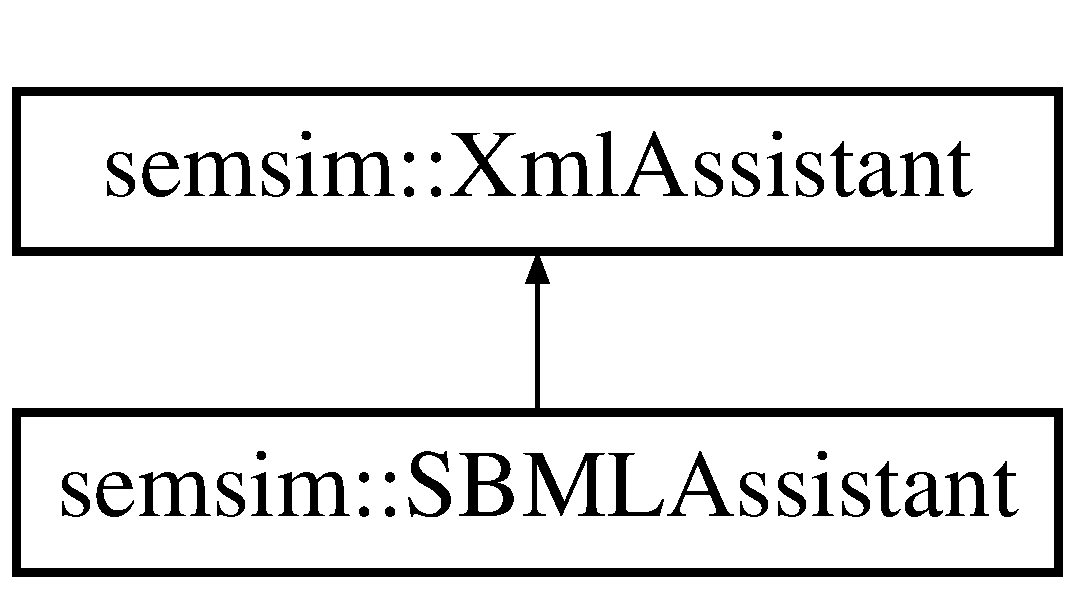
\includegraphics[height=2.000000cm]{classsemsim_1_1SBMLAssistant}
\end{center}
\end{figure}
\subsection*{Public Member Functions}
\begin{DoxyCompactItemize}
\item 
\mbox{\Hypertarget{classsemsim_1_1SBMLAssistant_a9e5e7db77689291f069dd8cbafa70296}\label{classsemsim_1_1SBMLAssistant_a9e5e7db77689291f069dd8cbafa70296}} 
std\+::vector$<$ std\+::string $>$ {\bfseries get\+Valid\+Elements} () const override
\end{DoxyCompactItemize}


The documentation for this class was generated from the following files\+:\begin{DoxyCompactItemize}
\item 
src/semsim/Semsim\+Xml\+Assistant.\+h\item 
src/semsim/Semsim\+Xml\+Assistant.\+cpp\end{DoxyCompactItemize}

\hypertarget{classsemsim_1_1SemSim}{}\section{semsim\+:\+:Sem\+Sim Class Reference}
\label{classsemsim_1_1SemSim}\index{semsim\+::\+Sem\+Sim@{semsim\+::\+Sem\+Sim}}
Inheritance diagram for semsim\+:\+:Sem\+Sim\+:\begin{figure}[H]
\begin{center}
\leavevmode
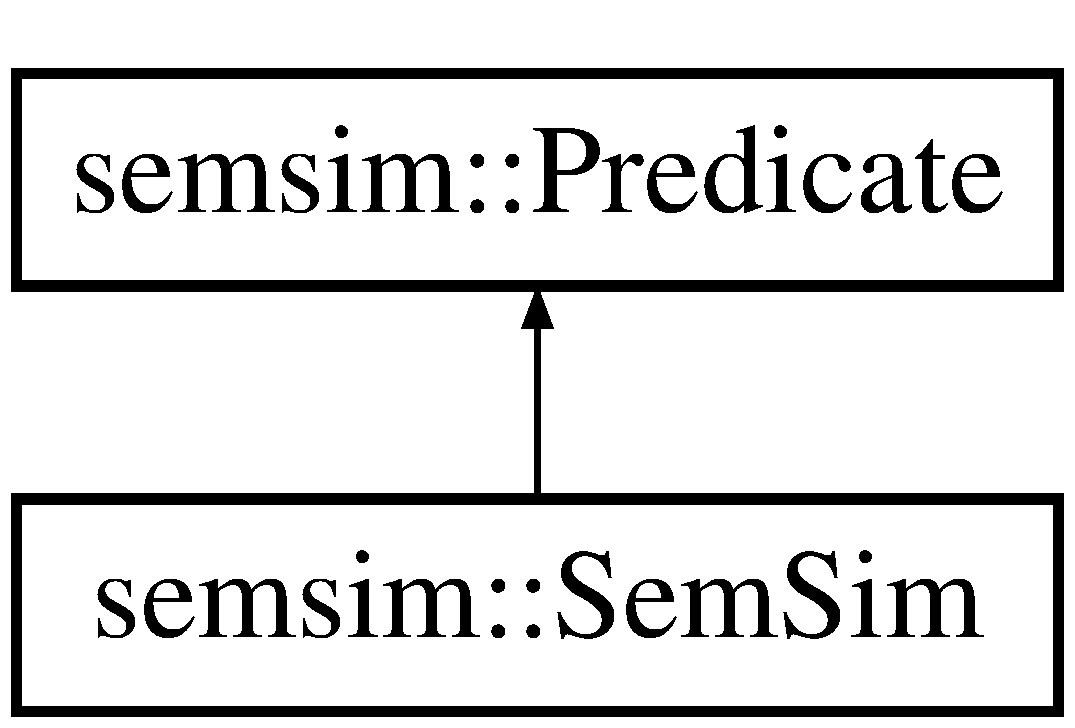
\includegraphics[height=2.000000cm]{classsemsim_1_1SemSim}
\end{center}
\end{figure}
\subsection*{Public Member Functions}
\begin{DoxyCompactItemize}
\item 
\mbox{\Hypertarget{classsemsim_1_1SemSim_ad9f48f4dde6bc27789826a29adf203ab}\label{classsemsim_1_1SemSim_ad9f48f4dde6bc27789826a29adf203ab}} 
{\bfseries Sem\+Sim} (const std\+::string \&term)
\item 
\mbox{\Hypertarget{classsemsim_1_1SemSim_a8df80cef39d98e83dab0c8c7bdae5d47}\label{classsemsim_1_1SemSim_a8df80cef39d98e83dab0c8c7bdae5d47}} 
void {\bfseries verify} ()
\end{DoxyCompactItemize}
\subsection*{Public Attributes}
\begin{DoxyCompactItemize}
\item 
std\+::vector$<$ std\+::string $>$ {\bfseries valid\+\_\+terms\+\_\+}
\end{DoxyCompactItemize}
\subsection*{Additional Inherited Members}


\subsection{Member Data Documentation}
\mbox{\Hypertarget{classsemsim_1_1SemSim_aa48e26f272827d7737f2bb9236c78102}\label{classsemsim_1_1SemSim_aa48e26f272827d7737f2bb9236c78102}} 
\index{semsim\+::\+Sem\+Sim@{semsim\+::\+Sem\+Sim}!valid\+\_\+terms\+\_\+@{valid\+\_\+terms\+\_\+}}
\index{valid\+\_\+terms\+\_\+@{valid\+\_\+terms\+\_\+}!semsim\+::\+Sem\+Sim@{semsim\+::\+Sem\+Sim}}
\subsubsection{\texorpdfstring{valid\+\_\+terms\+\_\+}{valid\_terms\_}}
{\footnotesize\ttfamily std\+::vector$<$std\+::string$>$ semsim\+::\+Sem\+Sim\+::valid\+\_\+terms\+\_\+}

{\bfseries Initial value\+:}
\begin{DoxyCode}
\{
                \textcolor{stringliteral}{"hasSourceParticipant"},
                \textcolor{stringliteral}{"hasSinkParticipant"},
                \textcolor{stringliteral}{"hasMediatorParticipant"},
                \textcolor{stringliteral}{"hasMultiplier"},
                \textcolor{stringliteral}{"hasPhysicalEntityReference"},
        \}
\end{DoxyCode}


The documentation for this class was generated from the following files\+:\begin{DoxyCompactItemize}
\item 
src/semsim/Predicate.\+h\item 
src/semsim/Predicate.\+cpp\end{DoxyCompactItemize}

\hypertarget{classsemsim_1_1SemsimUtils}{}\section{semsim\+:\+:Semsim\+Utils Class Reference}
\label{classsemsim_1_1SemsimUtils}\index{semsim\+::\+Semsim\+Utils@{semsim\+::\+Semsim\+Utils}}
\subsection*{Static Public Member Functions}
\begin{DoxyCompactItemize}
\item 
\mbox{\Hypertarget{classsemsim_1_1SemsimUtils_ac8367db330391787072c851985398805}\label{classsemsim_1_1SemsimUtils_ac8367db330391787072c851985398805}} 
static bool {\bfseries exists} (const std\+::string \&filename)
\item 
\mbox{\Hypertarget{classsemsim_1_1SemsimUtils_a1693cfd51439a6cc8c1144e82c2e83b3}\label{classsemsim_1_1SemsimUtils_a1693cfd51439a6cc8c1144e82c2e83b3}} 
static int {\bfseries remove\+File} (const std\+::string \&filename)
\item 
\mbox{\Hypertarget{classsemsim_1_1SemsimUtils_af758a31b9f4de651636587414c071059}\label{classsemsim_1_1SemsimUtils_af758a31b9f4de651636587414c071059}} 
static void {\bfseries remove\+If\+Exists} (const std\+::string \&filename)
\item 
\mbox{\Hypertarget{classsemsim_1_1SemsimUtils_a8eca0e4f3abb89c3577a8e099de8b9ba}\label{classsemsim_1_1SemsimUtils_a8eca0e4f3abb89c3577a8e099de8b9ba}} 
static void {\bfseries download} (const std\+::string \&url, std\+::string filename)
\item 
\mbox{\Hypertarget{classsemsim_1_1SemsimUtils_a07824a843bec362a8b6f7de1154068d5}\label{classsemsim_1_1SemsimUtils_a07824a843bec362a8b6f7de1154068d5}} 
static std\+::vector$<$ std\+::string $>$ {\bfseries split\+String\+By} (const std\+::string \&str, char delimiter)
\item 
\mbox{\Hypertarget{classsemsim_1_1SemsimUtils_a24671cf37888fe4b32188bd6759056d9}\label{classsemsim_1_1SemsimUtils_a24671cf37888fe4b32188bd6759056d9}} 
static std\+::string {\bfseries generate\+Unique\+Metaid} (librdf\+\_\+model $\ast$model, std\+::string metaid\+\_\+base, std\+::vector$<$ std\+::string $>$ exclusions=std\+::vector$<$ std\+::string $>$())
\item 
\mbox{\Hypertarget{classsemsim_1_1SemsimUtils_aa9435581e7fb3183edad803dbb2f5513}\label{classsemsim_1_1SemsimUtils_aa9435581e7fb3183edad803dbb2f5513}} 
static std\+::string {\bfseries add\+File\+Prefix\+To\+String} (std\+::string str)
\item 
\mbox{\Hypertarget{classsemsim_1_1SemsimUtils_a05a788ad4fb29a2f583fa1179abc15c0}\label{classsemsim_1_1SemsimUtils_a05a788ad4fb29a2f583fa1179abc15c0}} 
static std\+::string {\bfseries get\+Namespace\+From\+Uri} (const std\+::string \&uri)
\end{DoxyCompactItemize}


The documentation for this class was generated from the following files\+:\begin{DoxyCompactItemize}
\item 
src/semsim/Semsim\+Utils.\+h\item 
src/semsim/Semsim\+Utils.\+cpp\end{DoxyCompactItemize}

\hypertarget{classsemsim_1_1SemsimXmlAssistant}{}\section{semsim\+:\+:Semsim\+Xml\+Assistant Class Reference}
\label{classsemsim_1_1SemsimXmlAssistant}\index{semsim\+::\+Semsim\+Xml\+Assistant@{semsim\+::\+Semsim\+Xml\+Assistant}}
Inheritance diagram for semsim\+:\+:Semsim\+Xml\+Assistant\+:\begin{figure}[H]
\begin{center}
\leavevmode
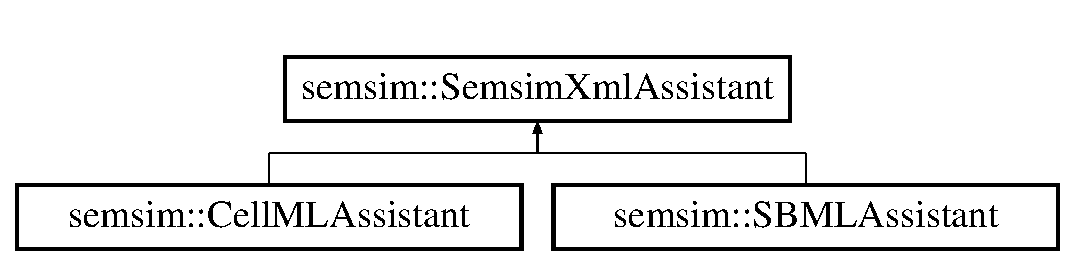
\includegraphics[height=2.000000cm]{classsemsim_1_1SemsimXmlAssistant}
\end{center}
\end{figure}
\subsection*{Public Member Functions}
\begin{DoxyCompactItemize}
\item 
\mbox{\Hypertarget{classsemsim_1_1SemsimXmlAssistant_a815b21c127616702584895612b971674}\label{classsemsim_1_1SemsimXmlAssistant_a815b21c127616702584895612b971674}} 
{\bfseries Semsim\+Xml\+Assistant} (std\+::string xml, std\+::string base=\char`\"{}Meta\+ID\char`\"{}, int metaid\+\_\+num\+\_\+digits=4)
\item 
\mbox{\Hypertarget{classsemsim_1_1SemsimXmlAssistant_a88422a4f11743c563a7ce776f4b9792a}\label{classsemsim_1_1SemsimXmlAssistant_a88422a4f11743c563a7ce776f4b9792a}} 
std\+::pair$<$ std\+::string, std\+::vector$<$ std\+::string $>$ $>$ {\bfseries add\+Meta\+Ids} ()
\item 
\mbox{\Hypertarget{classsemsim_1_1SemsimXmlAssistant_a428ad685b04bf7d4fb0beed12714c8b1}\label{classsemsim_1_1SemsimXmlAssistant_a428ad685b04bf7d4fb0beed12714c8b1}} 
virtual std\+::vector$<$ std\+::string $>$ {\bfseries get\+Valid\+Elements} () const
\end{DoxyCompactItemize}


The documentation for this class was generated from the following files\+:\begin{DoxyCompactItemize}
\item 
src/semsim/Semsim\+Xml\+Assistant.\+h\item 
src/semsim/Semsim\+Xml\+Assistant.\+cpp\end{DoxyCompactItemize}

\hypertarget{classsemsim_1_1SemsimXmlAssistantFactory}{}\section{semsim\+:\+:Semsim\+Xml\+Assistant\+Factory Class Reference}
\label{classsemsim_1_1SemsimXmlAssistantFactory}\index{semsim\+::\+Semsim\+Xml\+Assistant\+Factory@{semsim\+::\+Semsim\+Xml\+Assistant\+Factory}}
\subsection*{Static Public Member Functions}
\begin{DoxyCompactItemize}
\item 
\mbox{\Hypertarget{classsemsim_1_1SemsimXmlAssistantFactory_af24bed5c527a0a05d0fe579f1faa6dfd}\label{classsemsim_1_1SemsimXmlAssistantFactory_af24bed5c527a0a05d0fe579f1faa6dfd}} 
static Xml\+Assistant\+Ptr {\bfseries generate} (const std\+::string \&xml, Semsim\+Xml\+Type type)
\end{DoxyCompactItemize}


The documentation for this class was generated from the following files\+:\begin{DoxyCompactItemize}
\item 
src/semsim/Semsim\+Xml\+Assistant.\+h\item 
src/semsim/Semsim\+Xml\+Assistant.\+cpp\end{DoxyCompactItemize}

\hypertarget{classsemsim_1_1SinkParticipant}{}\doxysection{semsim\+::Sink\+Participant Class Reference}
\label{classsemsim_1_1SinkParticipant}\index{semsim::SinkParticipant@{semsim::SinkParticipant}}
Inheritance diagram for semsim\+::Sink\+Participant\+:\begin{figure}[H]
                                                          \begin{center}
                                                              \leavevmode
                                                              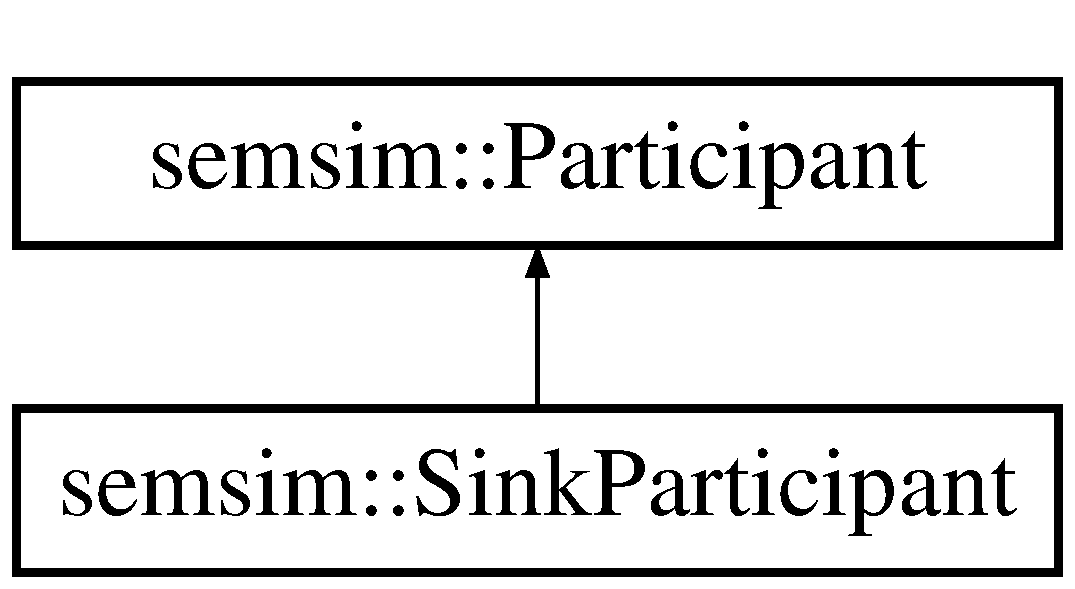
\includegraphics[height=2.000000cm]{classsemsim_1_1SinkParticipant}
                                                          \end{center}
\end{figure}
\doxysubsection*{Public Member Functions}
\begin{DoxyCompactItemize}
    \item
    \mbox{\Hypertarget{classsemsim_1_1SinkParticipant_a15037d52e6b1abfd72336f1209ddbcc9}\label{classsemsim_1_1SinkParticipant_a15037d52e6b1abfd72336f1209ddbcc9}}
    {\bfseries Sink\+Participant} (Librdf\+World world, Librdf\+Model model, std\+::string subject, double multiplier, std\+::string physical\+Entity\+Reference)
\end{DoxyCompactItemize}


The documentation for this class was generated from the following files\+:\begin{DoxyCompactItemize}
                                                                              \item
                                                                              src/semsim/Participant.\+h\item
                                                                              src/semsim/Participant.\+cpp
\end{DoxyCompactItemize}

\hypertarget{classsemsim_1_1SourceParticipant}{}\section{semsim\+:\+:Source\+Participant Class Reference}
\label{classsemsim_1_1SourceParticipant}\index{semsim\+::\+Source\+Participant@{semsim\+::\+Source\+Participant}}
Inheritance diagram for semsim\+:\+:Source\+Participant\+:\begin{figure}[H]
\begin{center}
\leavevmode
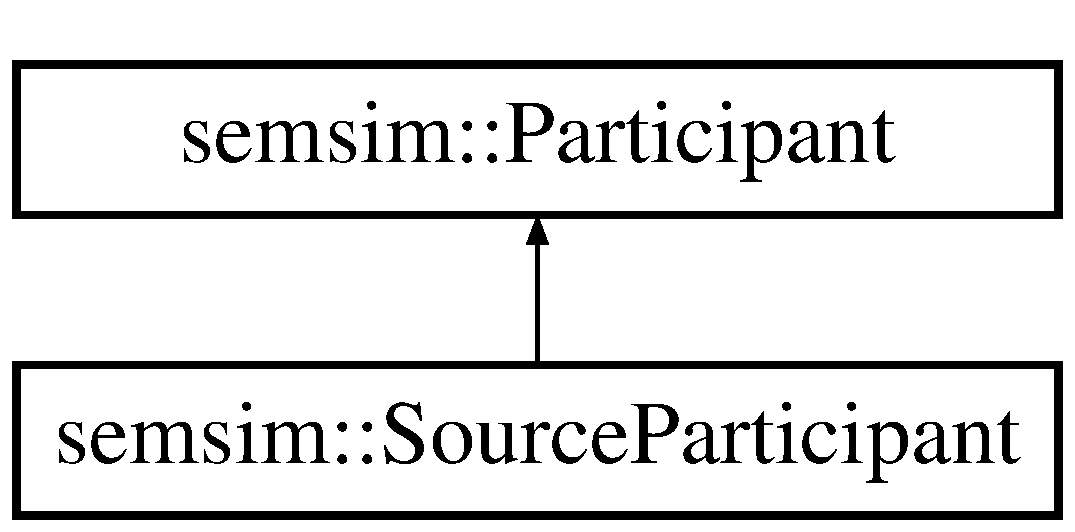
\includegraphics[height=2.000000cm]{classsemsim_1_1SourceParticipant}
\end{center}
\end{figure}
\subsection*{Public Member Functions}
\begin{DoxyCompactItemize}
\item 
\mbox{\Hypertarget{classsemsim_1_1SourceParticipant_a7e942f26b1bf916f0441d353f80833a1}\label{classsemsim_1_1SourceParticipant_a7e942f26b1bf916f0441d353f80833a1}} 
{\bfseries Source\+Participant} (librdf\+\_\+model $\ast$model, std\+::string subject, double multiplier, std\+::string physical\+Entity\+Reference)
\end{DoxyCompactItemize}


The documentation for this class was generated from the following files\+:\begin{DoxyCompactItemize}
\item 
src/semsim/Participant.\+h\item 
src/semsim/Participant.\+cpp\end{DoxyCompactItemize}

\hypertarget{classsemsim_1_1Subject}{}\section{semsim\+:\+:Subject Class Reference}
\label{classsemsim_1_1Subject}\index{semsim\+::\+Subject@{semsim\+::\+Subject}}
\subsection*{Public Member Functions}
\begin{DoxyCompactItemize}
\item 
\mbox{\Hypertarget{classsemsim_1_1Subject_aa17c4b8d8a774d815129eb78ee9be4c6}\label{classsemsim_1_1Subject_aa17c4b8d8a774d815129eb78ee9be4c6}} 
{\bfseries Subject} (\hyperlink{classredland_1_1LibrdfNode}{Librdf\+Node} node)
\item 
\mbox{\Hypertarget{classsemsim_1_1Subject_a190fa201096714efe10354f73e340146}\label{classsemsim_1_1Subject_a190fa201096714efe10354f73e340146}} 
librdf\+\_\+node $\ast$ {\bfseries get\+Node} () const
\item 
\mbox{\Hypertarget{classsemsim_1_1Subject_affe03a33bb3ef32bce77e26b24f018f8}\label{classsemsim_1_1Subject_affe03a33bb3ef32bce77e26b24f018f8}} 
void {\bfseries set\+Node} (librdf\+\_\+node $\ast$node)
\item 
\mbox{\Hypertarget{classsemsim_1_1Subject_a4244a40a89fb9a3dd6ffff35cd95f7ca}\label{classsemsim_1_1Subject_a4244a40a89fb9a3dd6ffff35cd95f7ca}} 
std\+::string {\bfseries str} () const
\item 
\mbox{\Hypertarget{classsemsim_1_1Subject_aecfc41aed32eb5a2a5c5eadc814192d2}\label{classsemsim_1_1Subject_aecfc41aed32eb5a2a5c5eadc814192d2}} 
bool {\bfseries is\+Set} () const
\item 
\mbox{\Hypertarget{classsemsim_1_1Subject_ad522878616f2ed76b3a807b9374ea090}\label{classsemsim_1_1Subject_ad522878616f2ed76b3a807b9374ea090}} 
void {\bfseries free} ()
\end{DoxyCompactItemize}
\subsection*{Static Public Member Functions}
\begin{DoxyCompactItemize}
\item 
\mbox{\Hypertarget{classsemsim_1_1Subject_ad119bbf8b29abea7a23efc1df6268052}\label{classsemsim_1_1Subject_ad119bbf8b29abea7a23efc1df6268052}} 
static \hyperlink{classsemsim_1_1Subject}{Subject} {\bfseries from\+Raw\+Ptr} (librdf\+\_\+node $\ast$node)
\item 
\mbox{\Hypertarget{classsemsim_1_1Subject_a180f5d9c5523f96711dd4bd363e0b60b}\label{classsemsim_1_1Subject_a180f5d9c5523f96711dd4bd363e0b60b}} 
static \hyperlink{classsemsim_1_1Subject}{Subject} {\bfseries from\+Uri} (const std\+::string \&uri)
\item 
\mbox{\Hypertarget{classsemsim_1_1Subject_a3a117e493ff15d93414016bb2d8730ec}\label{classsemsim_1_1Subject_a3a117e493ff15d93414016bb2d8730ec}} 
static \hyperlink{classsemsim_1_1Subject}{Subject} {\bfseries from\+Blank} (const std\+::string \&blank)
\end{DoxyCompactItemize}


The documentation for this class was generated from the following files\+:\begin{DoxyCompactItemize}
\item 
src/semsim/Subject.\+h\item 
src/semsim/Subject.\+cpp\end{DoxyCompactItemize}

\hypertarget{classsemsim_1_1Triple}{}\section{semsim\+:\+:Triple Class Reference}
\label{classsemsim_1_1Triple}\index{semsim\+::\+Triple@{semsim\+::\+Triple}}
Inheritance diagram for semsim\+:\+:Triple\+:\begin{figure}[H]
\begin{center}
\leavevmode
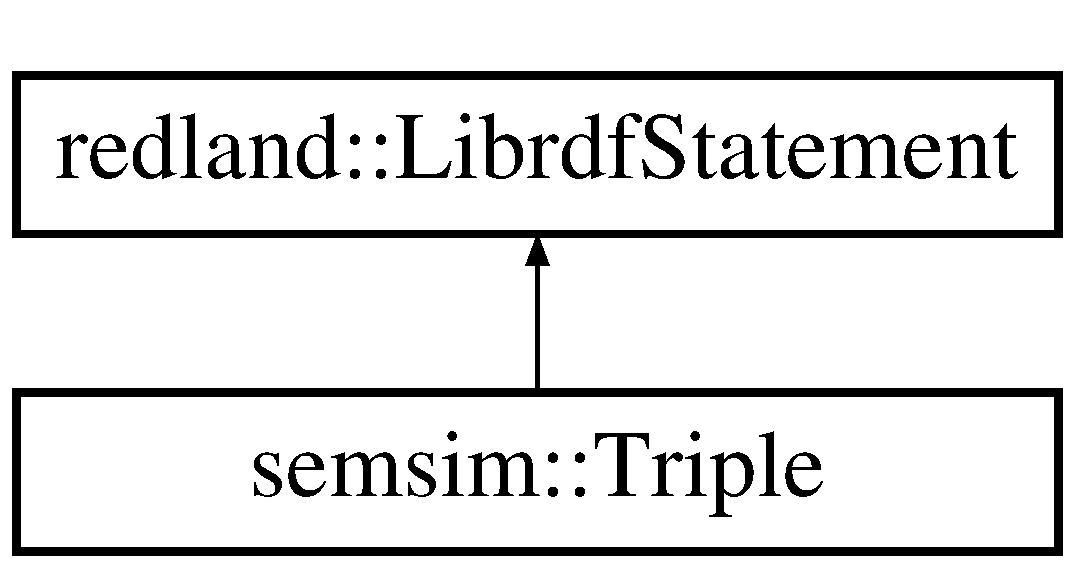
\includegraphics[height=2.000000cm]{classsemsim_1_1Triple}
\end{center}
\end{figure}
\subsection*{Public Member Functions}
\begin{DoxyCompactItemize}
\item 
\mbox{\Hypertarget{classsemsim_1_1Triple_a2d73ce89601f4ff3df0abe8c9646876c}\label{classsemsim_1_1Triple_a2d73ce89601f4ff3df0abe8c9646876c}} 
{\bfseries Triple} (const \hyperlink{classsemsim_1_1Subject}{Subject} \&subject, const Predicate\+Ptr \&predicate\+\_\+ptr, const \hyperlink{classsemsim_1_1Resource}{Resource} \&resource)
\item 
\mbox{\Hypertarget{classsemsim_1_1Triple_a633f2253a4ea8689721aeeb0929a4e26}\label{classsemsim_1_1Triple_a633f2253a4ea8689721aeeb0929a4e26}} 
{\bfseries Triple} (librdf\+\_\+node $\ast$subject, librdf\+\_\+node $\ast$predicate, librdf\+\_\+node $\ast$resource)
\item 
\mbox{\Hypertarget{classsemsim_1_1Triple_a20ba537cd620f4fec9bc56eb29662d23}\label{classsemsim_1_1Triple_a20ba537cd620f4fec9bc56eb29662d23}} 
std\+::string {\bfseries str} (const std\+::string \&format=\char`\"{}rdfxml-\/abbrev\char`\"{}, const std\+::string \&base=\char`\"{}file\+://./annotations.\+rdf\char`\"{})
\item 
\mbox{\Hypertarget{classsemsim_1_1Triple_ad2b2ab0b15a970f5dc95a25e1ec61f1f}\label{classsemsim_1_1Triple_ad2b2ab0b15a970f5dc95a25e1ec61f1f}} 
\hyperlink{classsemsim_1_1Triple}{Triple} \& {\bfseries set\+About} (const std\+::string \&about)
\item 
\mbox{\Hypertarget{classsemsim_1_1Triple_a972f806fbf6e71f60f6b6b7ba433c79c}\label{classsemsim_1_1Triple_a972f806fbf6e71f60f6b6b7ba433c79c}} 
std\+::string {\bfseries get\+About} () const
\item 
\mbox{\Hypertarget{classsemsim_1_1Triple_a12bbba125df06854a1954ccff5be72e9}\label{classsemsim_1_1Triple_a12bbba125df06854a1954ccff5be72e9}} 
std\+::shared\+\_\+ptr$<$ librdf\+\_\+statement $>$ {\bfseries get\+Statement} () const
\item 
\mbox{\Hypertarget{classsemsim_1_1Triple_af39ecc1713db90ccfbad436eb52fe900}\label{classsemsim_1_1Triple_af39ecc1713db90ccfbad436eb52fe900}} 
\hyperlink{classsemsim_1_1Triple}{Triple} \& {\bfseries set\+Predicate} (const std\+::string \&namespace\+\_\+, const std\+::string \&term)
\item 
\mbox{\Hypertarget{classsemsim_1_1Triple_ad85dc3e3538da54fb96387a3135b8f78}\label{classsemsim_1_1Triple_ad85dc3e3538da54fb96387a3135b8f78}} 
\hyperlink{classsemsim_1_1Triple}{Triple} \& {\bfseries set\+Resource\+Literal} (const std\+::string \&literal)
\item 
\mbox{\Hypertarget{classsemsim_1_1Triple_a09a6b7c88633a87f489a8f125897935a}\label{classsemsim_1_1Triple_a09a6b7c88633a87f489a8f125897935a}} 
\hyperlink{classsemsim_1_1Triple}{Triple} \& {\bfseries set\+Resource\+Uri} (const std\+::string \&identifiers\+\_\+uri)
\item 
\mbox{\Hypertarget{classsemsim_1_1Triple_a5f62f4d7c1dc8877fa7861d0b399c696}\label{classsemsim_1_1Triple_a5f62f4d7c1dc8877fa7861d0b399c696}} 
\hyperlink{classsemsim_1_1Triple}{Triple} \& {\bfseries set\+Resource\+Blank} (const std\+::string \&blank\+\_\+id)
\item 
\mbox{\Hypertarget{classsemsim_1_1Triple_a0dd977326ab305c6327a62b8c009f60f}\label{classsemsim_1_1Triple_a0dd977326ab305c6327a62b8c009f60f}} 
bool {\bfseries is\+Empty} ()
\item 
\mbox{\Hypertarget{classsemsim_1_1Triple_ac61be91d0c4e21a033a0052f0bab7487}\label{classsemsim_1_1Triple_ac61be91d0c4e21a033a0052f0bab7487}} 
\hyperlink{classsemsim_1_1Triple}{Triple} \& {\bfseries set\+Predicate} (const std\+::string \&uri)
\end{DoxyCompactItemize}
\subsection*{Static Public Member Functions}
\begin{DoxyCompactItemize}
\item 
\mbox{\Hypertarget{classsemsim_1_1Triple_aec7e299bc50b39bd0421da8ab56d95f9}\label{classsemsim_1_1Triple_aec7e299bc50b39bd0421da8ab56d95f9}} 
static \hyperlink{classsemsim_1_1Triple}{Triple} {\bfseries from\+Raw\+Statement\+Ptr} (librdf\+\_\+statement $\ast$statement)
\end{DoxyCompactItemize}
\subsection*{Additional Inherited Members}


The documentation for this class was generated from the following files\+:\begin{DoxyCompactItemize}
\item 
src/semsim/Triple.\+h\item 
src/semsim/Triple.\+cpp\end{DoxyCompactItemize}

\hypertarget{classsemsim_1_1Triples}{}\section{semsim\+:\+:Triples Class Reference}
\label{classsemsim_1_1Triples}\index{semsim\+::\+Triples@{semsim\+::\+Triples}}
\subsection*{Public Member Functions}
\begin{DoxyCompactItemize}
\item 
\mbox{\Hypertarget{classsemsim_1_1Triples_a620eba7d105212f69f762e9614c82928}\label{classsemsim_1_1Triples_a620eba7d105212f69f762e9614c82928}} 
{\bfseries Triples} (\hyperlink{classsemsim_1_1Triple}{Triple} triple)
\item 
\mbox{\Hypertarget{classsemsim_1_1Triples_a09d81ba233bf8a3ca5a9ede2df74c825}\label{classsemsim_1_1Triples_a09d81ba233bf8a3ca5a9ede2df74c825}} 
{\bfseries Triples} (std\+::vector$<$ \hyperlink{classsemsim_1_1Triple}{Triple} $>$ triples)
\item 
\mbox{\Hypertarget{classsemsim_1_1Triples_a6a93d787c250b81592bb9b5fa30fdec2}\label{classsemsim_1_1Triples_a6a93d787c250b81592bb9b5fa30fdec2}} 
void {\bfseries push\+\_\+back} (\hyperlink{classsemsim_1_1Triple}{Triple} triple)
\item 
\mbox{\Hypertarget{classsemsim_1_1Triples_a2387f43385258c96bd68ca38d1a53c94}\label{classsemsim_1_1Triples_a2387f43385258c96bd68ca38d1a53c94}} 
void {\bfseries emplace\+\_\+back} (\hyperlink{classsemsim_1_1Subject}{Subject} subject, const Predicate\+Ptr \&predicate\+Ptr, const \hyperlink{classsemsim_1_1Resource}{Resource} \&resource)
\item 
\mbox{\Hypertarget{classsemsim_1_1Triples_a69c8a69a0dcffc60e510b731a0ffec69}\label{classsemsim_1_1Triples_a69c8a69a0dcffc60e510b731a0ffec69}} 
void {\bfseries emplace\+\_\+back} (\hyperlink{classsemsim_1_1Subject}{Subject} subject, const \hyperlink{classsemsim_1_1Predicate}{Predicate} \&predicate, const \hyperlink{classsemsim_1_1Resource}{Resource} \&resource)
\item 
\mbox{\Hypertarget{classsemsim_1_1Triples_a139321c0554ce0cf98d2fccc82599653}\label{classsemsim_1_1Triples_a139321c0554ce0cf98d2fccc82599653}} 
void {\bfseries emplace\+\_\+back} (\hyperlink{classsemsim_1_1Subject}{Subject} subject, \hyperlink{classsemsim_1_1BiomodelsBiologyQualifier}{Biomodels\+Biology\+Qualifier} predicate, const \hyperlink{classsemsim_1_1Resource}{Resource} \&resource)
\item 
\mbox{\Hypertarget{classsemsim_1_1Triples_a7a7839f22cac425a78e6b4c95fa7d423}\label{classsemsim_1_1Triples_a7a7839f22cac425a78e6b4c95fa7d423}} 
void {\bfseries emplace\+\_\+back} (\hyperlink{classsemsim_1_1Subject}{Subject} subject, \hyperlink{classsemsim_1_1BiomodelsModelQualifier}{Biomodels\+Model\+Qualifier} predicate, const \hyperlink{classsemsim_1_1Resource}{Resource} \&resource)
\item 
\mbox{\Hypertarget{classsemsim_1_1Triples_a83049cf0e93d420a318bd041ec5410fb}\label{classsemsim_1_1Triples_a83049cf0e93d420a318bd041ec5410fb}} 
void {\bfseries emplace\+\_\+back} (\hyperlink{classsemsim_1_1Subject}{Subject} subject, \hyperlink{classsemsim_1_1DCTerm}{D\+C\+Term} predicate, const \hyperlink{classsemsim_1_1Resource}{Resource} \&resource)
\item 
\mbox{\Hypertarget{classsemsim_1_1Triples_aceaa9df401907b19d286ae8be29a4ed1}\label{classsemsim_1_1Triples_aceaa9df401907b19d286ae8be29a4ed1}} 
void {\bfseries emplace\+\_\+back} (\hyperlink{classsemsim_1_1Subject}{Subject} subject, \hyperlink{classsemsim_1_1SemSim}{Sem\+Sim} predicate, const \hyperlink{classsemsim_1_1Resource}{Resource} \&resource)
\item 
\mbox{\Hypertarget{classsemsim_1_1Triples_a0cdb24ded3d2c8bcec95a41cfd8f14ec}\label{classsemsim_1_1Triples_a0cdb24ded3d2c8bcec95a41cfd8f14ec}} 
void {\bfseries emplace\+\_\+back} (librdf\+\_\+node $\ast$subject, librdf\+\_\+node $\ast$predicate, librdf\+\_\+node $\ast$resource)
\item 
\mbox{\Hypertarget{classsemsim_1_1Triples_a95177537847688d33f83302a65767982}\label{classsemsim_1_1Triples_a95177537847688d33f83302a65767982}} 
std\+::vector$<$ std\+::string $>$ {\bfseries get\+Subjects\+Str} ()
\item 
\mbox{\Hypertarget{classsemsim_1_1Triples_aa51480fb718cd5b47a2c96fc99a10c2c}\label{classsemsim_1_1Triples_aa51480fb718cd5b47a2c96fc99a10c2c}} 
std\+::vector$<$ std\+::string $>$ {\bfseries get\+Predicates} ()
\item 
\mbox{\Hypertarget{classsemsim_1_1Triples_ae4e47c0881214aec04987fada026f9ae}\label{classsemsim_1_1Triples_ae4e47c0881214aec04987fada026f9ae}} 
std\+::vector$<$ std\+::string $>$ {\bfseries get\+Resources} ()
\item 
\mbox{\Hypertarget{classsemsim_1_1Triples_a9787be0290ba6519cc4f71b28ce280f6}\label{classsemsim_1_1Triples_a9787be0290ba6519cc4f71b28ce280f6}} 
int {\bfseries size} ()
\item 
\mbox{\Hypertarget{classsemsim_1_1Triples_a7c107f7dd600189cff1b0abf6bdd5e72}\label{classsemsim_1_1Triples_a7c107f7dd600189cff1b0abf6bdd5e72}} 
Shared\+Triple\+Vector\+::iterator {\bfseries begin} ()
\item 
\mbox{\Hypertarget{classsemsim_1_1Triples_a9551a7d3ecc878b6ff87ddd2c52d6481}\label{classsemsim_1_1Triples_a9551a7d3ecc878b6ff87ddd2c52d6481}} 
Shared\+Triple\+Vector\+::iterator {\bfseries end} ()
\item 
\mbox{\Hypertarget{classsemsim_1_1Triples_a3fce442d97360b0c6ccb55fdf11f0bf2}\label{classsemsim_1_1Triples_a3fce442d97360b0c6ccb55fdf11f0bf2}} 
std\+::string {\bfseries str} (const std\+::string \&format=\char`\"{}rdfxml-\/abbrev\char`\"{}, std\+::string base=\char`\"{}file\+://./annotations.\+rdf\char`\"{})
\item 
\mbox{\Hypertarget{classsemsim_1_1Triples_afb9f000468cbe6c68f6c5706f0b2c781}\label{classsemsim_1_1Triples_afb9f000468cbe6c68f6c5706f0b2c781}} 
void {\bfseries push\+\_\+back} (const std\+::shared\+\_\+ptr$<$ \hyperlink{classsemsim_1_1Triple}{Triple} $>$ \&triple)
\end{DoxyCompactItemize}


The documentation for this class was generated from the following files\+:\begin{DoxyCompactItemize}
\item 
src/semsim/Triples.\+h\item 
src/semsim/Triples.\+cpp\end{DoxyCompactItemize}

\hypertarget{classsemsim_1_1ValueException}{}\section{semsim\+:\+:Value\+Exception Class Reference}
\label{classsemsim_1_1ValueException}\index{semsim\+::\+Value\+Exception@{semsim\+::\+Value\+Exception}}
Inheritance diagram for semsim\+:\+:Value\+Exception\+:\begin{figure}[H]
\begin{center}
\leavevmode
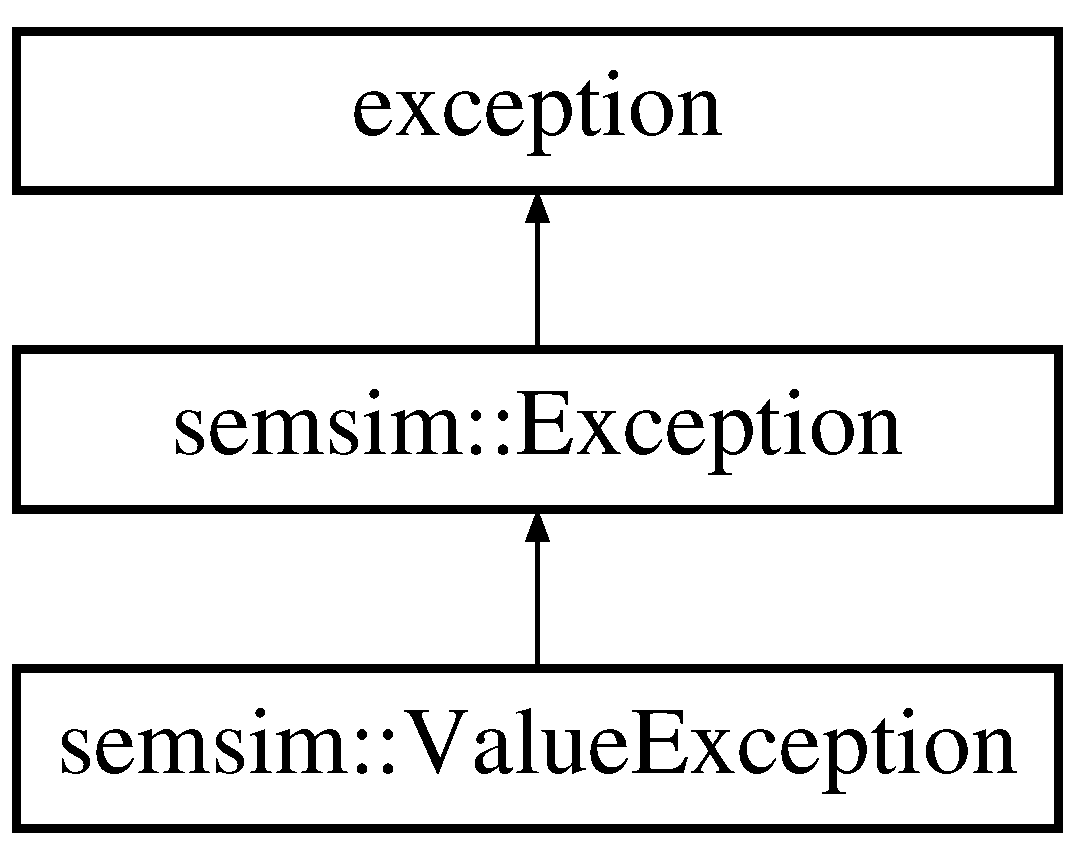
\includegraphics[height=3.000000cm]{classsemsim_1_1ValueException}
\end{center}
\end{figure}
\subsection*{Additional Inherited Members}


The documentation for this class was generated from the following file\+:\begin{DoxyCompactItemize}
\item 
src/semsim/Error.\+h\end{DoxyCompactItemize}

\hypertarget{classredland_1_1World}{}\section{redland\+:\+:World Class Reference}
\label{classredland_1_1World}\index{redland\+::\+World@{redland\+::\+World}}
\subsection*{Static Public Member Functions}
\begin{DoxyCompactItemize}
\item 
\mbox{\Hypertarget{classredland_1_1World_ad7618363c9b7da4c87367707c1a159d7}\label{classredland_1_1World_ad7618363c9b7da4c87367707c1a159d7}} 
static librdf\+\_\+world $\ast$ {\bfseries get\+World} ()
\item 
\mbox{\Hypertarget{classredland_1_1World_aac0ce4018279ced7b38a36d74bb10cec}\label{classredland_1_1World_aac0ce4018279ced7b38a36d74bb10cec}} 
static raptor\+\_\+world $\ast$ {\bfseries get\+Raptor} ()
\item 
\mbox{\Hypertarget{classredland_1_1World_ade64918f10ee6ee0f5b8a0cb2e01666b}\label{classredland_1_1World_ade64918f10ee6ee0f5b8a0cb2e01666b}} 
static void {\bfseries free} (librdf\+\_\+world $\ast$world)
\end{DoxyCompactItemize}


The documentation for this class was generated from the following files\+:\begin{DoxyCompactItemize}
\item 
src/redland/\+Redland\+A\+P\+I\+Wrapper/src/World.\+h\item 
src/redland/\+Redland\+A\+P\+I\+Wrapper/src/World.\+cpp\end{DoxyCompactItemize}

%--- End generated contents ---

% Index
\backmatter
\newpage
\phantomsection
\clearemptydoublepage
\addcontentsline{toc}{chapter}{Index}
\printindex

\end{document}
